% Формат А4, 14pt (ГОСТ Р 7.0.11-2011, 5.3.6)
\documentclass[a4paper,14pt]{extreport}

%%%%%%%%%%%%%%%%%%%%%%%%%%%%%%%%%%%%%%%%%%%%%%%%%%%%%%
%%%% Файл упрощённых настроек шаблона диссертации %%%%
%%%%%%%%%%%%%%%%%%%%%%%%%%%%%%%%%%%%%%%%%%%%%%%%%%%%%%

%%%        Подключение пакетов                 %%%
\usepackage{ifthen}                 % добавляет ifthenelse
%%% Инициализирование переменных, не трогать!  %%%
\newcounter{bibliosel}
%%%%%%%%%%%%%%%%%%%%%%%%%%%%%%%%%%%%%%%%%%%%%%%%%%

%%% Область упрощённого управления оформлением %%%

%% Библиография
\setcounter{bibliosel}{0}           % 0 --- встроенная реализация с загрузкой файла через движок bibtex8; 1 --- реализация пакетом biblatex через движок biber
               % Упрощённые настройки шаблона 

%%% Проверка используемого TeX-движка %%%
\usepackage{iftex}
\newif\ifxetexorluatex   % определяем новый условный оператор (http://tex.stackexchange.com/a/47579/79756)
\ifXeTeX
    \xetexorluatextrue
\else
    \ifLuaTeX
        \xetexorluatextrue
    \else
        \xetexorluatexfalse
    \fi
\fi

%%% Поля и разметка страницы %%%
\usepackage{pdflscape}                              % Для включения альбомных страниц
\usepackage{geometry}                               % Для последующего задания полей

%%% Математические пакеты %%%
\usepackage{amsthm,amsfonts,amsmath,amssymb,amscd}  % Математические дополнения от AMS
\usepackage{mathtools}                              % Добавляет окружение multlined

%%%% Установки для размера шрифта 14 pt %%%%
%% Формирование переменных и констант для сравнения (один раз для всех подключаемых файлов)%%
%% должно располагаться до вызова пакета fontspec или polyglossia, потому что они сбивают его работу
\newlength{\curtextsize}
\newlength{\bigtextsize}
\setlength{\bigtextsize}{13.9pt}

\makeatletter
%\show\f@size                                       % неплохо для отслеживания, но вызывает стопорение процесса, если документ компилируется без команды  -interaction=nonstopmode 
\setlength{\curtextsize}{\f@size pt}
\makeatother

%%% Кодировки и шрифты %%%
\ifxetexorluatex
    \usepackage{polyglossia}                        % Поддержка многоязычности (fontspec подгружается автоматически)
\else
    \RequirePDFTeX                                  % tests for PDFTEX use and throws an error if a different engine is being used
    \usepackage{cmap}                               % Улучшенный поиск русских слов в полученном pdf-файле
    \usepackage[T2A]{fontenc}                       % Поддержка русских букв
    \usepackage[utf8]{inputenc}                     % Кодировка utf8
    \usepackage[english, russian]{babel}            % Языки: русский, английский
    \IfFileExists{pscyr.sty}{\usepackage{pscyr}}{}  % Красивые русские шрифты
\fi

%%% Оформление абзацев %%%
\usepackage{indentfirst}                            % Красная строка

%%% Цвета %%%
\usepackage[dvipsnames,usenames]{color}
\usepackage{colortbl}

%%% Таблицы %%%
\usepackage{longtable}                              % Длинные таблицы
\usepackage{multirow,makecell,array}                % Улучшенное форматирование таблиц
\usepackage{booktabs}                               % Возможность оформления таблиц в классическом книжном стиле (при правильном использовании не противоречит ГОСТ)

%%% Общее форматирование
\usepackage{soulutf8}                               % Поддержка переносоустойчивых подчёркиваний и зачёркиваний
\usepackage{icomma}                                 % Запятая в десятичных дробях


%%% Гиперссылки %%%
\usepackage{hyperref}

%%% Изображения %%%
\usepackage{graphicx}                               % Подключаем пакет работы с графикой

%%% Списки %%%
\usepackage{enumitem}

%%% Подписи %%%
\usepackage{caption}                                % Для управления подписями (рисунков и таблиц) % Может управлять номерами рисунков и таблиц с caption %Иногда может управлять заголовками в списках рисунков и таблиц
\usepackage{subcaption}                             % Работа с подрисунками и подобным

%%% Интервалы %%%
\usepackage[onehalfspacing]{setspace}               % Опция запуска пакета правит не только интервалы в обычном тексте, но и формульные

%%% Счётчики %%%
\usepackage[figure,table]{totalcount}               % Счётчик рисунков и таблиц
\usepackage{totcount}                               % Пакет создания счётчиков на основе последнего номера подсчитываемого элемента (может требовать дважды компилировать документ)
\usepackage{totpages}                               % Счётчик страниц, совместимый с hyperref (ссылается на номер последней страницы). Желательно ставить последним пакетом в преамбуле

  % Пакеты общие для диссертации и автореферата
%%% Колонтитулы %%%
\usepackage{fancyhdr}

%%% Прикладные пакеты %%% 
\usepackage{calc}               % Пакет для расчётов параметров, например длины
%\usepackage{etoolbox}          % ради функции patchcmd для управления списком литературы

\usepackage {interfaces-base}   % Набор базовых интерфейсов к некоторым пакетам, конкретные реализации загружаются в стиле

%%% Заголовки %%%
\usepackage{titlesec}           % Пакет настройки шрифтов заголовков в тексте

%%% Оглавление %%%
\usepackage{tocloft}

%%% Счётчики %%%
\usepackage{chngcntr}           % оперативная перенастройка счётчиков


         % Пакеты для диссертации
\usepackage{tabularx,tabulary}  %таблицы с автоматически подбирающейся шириной столбцов

% Листинги с исходным кодом программ
\usepackage{fancyvrb}
\usepackage{listings}

% Плавающие окружения. во многом лучше пакета float
\usepackage{floatrow}
        % Пакеты для специфических пользовательских задач
%%% Переопределение именований, чтобы можно было и в преамбуле использовать %%%
\renewcommand{\chaptername}{Chapter}
\renewcommand{\appendixname}{Appendix} % (ГОСТ Р 7.0.11-2011, 5.7)
       % Переопределение именований, чтобы можно было и в преамбуле использовать
%%% Макет страницы %%%
% Выставляем значения полей (ГОСТ 7.0.11-2011, 5.3.7)
\geometry{a4paper,top=2cm,bottom=2cm,left=2.5cm,right=1cm}

%%% Кодировки и шрифты %%%
\ifxetexorluatex
    \setmainlanguage[babelshorthands=true]{english}  % Язык по-умолчанию English с поддержкой приятных команд пакета babel                
    \ifXeTeX
        \defaultfontfeatures{Ligatures=TeX,Mapping=tex-text}
    \else
        \defaultfontfeatures{Ligatures=TeX}
    \fi
    \setmainfont{Times New Roman}
    \newfontfamily\cyrillicfont{Times New Roman}
    \setsansfont{Arial}
    \newfontfamily\cyrillicfontsf{Arial}
    \setmonofont{Courier New}
    \newfontfamily\cyrillicfonttt{Courier New}
\else
    \IfFileExists{pscyr.sty}{\renewcommand{\rmdefault}{ftm}}{}
\fi

%%% Интервалы %%%
%linespread-реализация ближе к реализации полуторного интервала в ворде.
%setspace реализация заточена под шрифты 10, 11, 12pt, под остальные кегли хуже, но всё же ближе к типографской классике. 
%\linespread{1.3}                    % Полуторный интервал (ГОСТ Р 7.0.11-2011, 5.3.6)

%%% Выравнивание и переносы %%%
\sloppy                             % Избавляемся от переполнений
\clubpenalty=10000                  % Запрещаем разрыв страницы после первой строки абзаца
\widowpenalty=10000                 % Запрещаем разрыв страницы после последней строки абзаца

%%% Изображения %%%
\graphicspath{{images/}}            % Пути к изображениям

%%% Подписи %%%
\captionsetup{%
singlelinecheck=off,                % Многострочные подписи, например у таблиц
skip=2pt,                           % Вертикальная отбивка между подписью и содержимым рисунка или таблицы определяется ключом
justification=centering,            % Центрирование подписей, заданных командой \caption
}

%\precaption{\tabcapalign} % всегда идет перед подписью или \legend
%\captionnamefont{\normalfont\normalsize} % Шрифт надписи «Таблица #»; также определяет шрифт у \legend
%\captiondelim{\tablabelsep} % разделитель идентификатора с номером от наименования
%\captionstyle[\tabtitalign]{\tabtitalign}
%\captiontitlefont{\normalfont\normalsize} % Шрифт с текстом подписи

%%% Рисунки %%%
\DeclareCaptionLabelSeparator*{emdash}{~--- }             % (ГОСТ 2.105, 4.3.1)
\captionsetup[figure]{labelsep=emdash,font=onehalfspacing,position=bottom}

%%% Таблицы %%%
\DeclareCaptionFormat{tablecaption}{\raggedleft #1#2\\%   % Идентификатор таблицы справа, на отдельной строке
    \centering{#3}}                                       % Наименование таблицы строкой ниже и центрировано, без переносов
\DeclareCaptionFormat{tablenocaption}{\raggedleft #1#2%   % Идентификатор таблицы справа, на отдельной строке
}                                                         % Наименование таблицы отсутствует
\captionsetup[table]{format=tablecaption,labelsep=space,singlelinecheck=off,font=onehalfspacing,position=top}  % пробельный разделитьель идентификатора с номером от наименования, многострочные наименования и прочее
\DeclareCaptionLabelFormat{continued}{Сontinue of the table~#2}

%%% Подписи подрисунков %%%
\renewcommand{\thesubfigure}{\asbuk{subfigure}}           % Буквенные номера подрисунков
\captionsetup[subfigure]{font={normalsize},               % Шрифт подписи названий подрисунков (не отличается от основного)
    labelformat=brace,                                    % Формат обозначения подрисунка
    justification=centering,                              % Выключка подписей (форматирование), один из вариантов            
}
%\DeclareCaptionFont{font12pt}{\fontsize{12pt}{13pt}\selectfont} % объявляем шрифт 12pt для использования в подписях, тут же надо интерлиньяж объявлять, если не наследуется
%\captionsetup[subfigure]{font={font12pt}}                 % Шрифт подписи названий подрисунков (всегда 12pt)

%%% Цвета гиперссылок %%%
\definecolor{linkcolor}{rgb}{0.9,0,0}
\definecolor{citecolor}{rgb}{0,0.6,0}
\definecolor{urlcolor}{rgb}{0,0,1}

%%% Настройки гиперссылок %%%
\hypersetup{
    linktocpage=true,           % ссылки с номера страницы в оглавлении, списке таблиц и списке рисунков
%    pdfpagelabels=false,        % set PDF page labels (true|false)
    plainpages=false,           % Forces page anchors to be named by the Arabic form  of the page number, rather than the formatted form
    colorlinks,                 % ссылки отображаются раскрашенным текстом, а не раскрашенным прямоугольником, вокруг текста
    linkcolor={linkcolor},      % цвет ссылок типа ref, eqref и подобных
    citecolor={citecolor},      % цвет ссылок-цитат
    urlcolor={urlcolor},        % цвет гиперссылок
}

\ifLuaTeX
    \hypersetup{
        unicode,                % Unicode encoded PDF strings
    }
\fi

%%% Шаблон %%%
\DeclareRobustCommand{\todo}{\textcolor{red}}       % решаем проблему превращения названия цвета в результате \MakeUppercase, http://tex.stackexchange.com/a/187930/79756 , \DeclareRobustCommand protects \todo from expanding inside \MakeUppercase
\setlength{\parindent}{2.5em}                       % Абзацный отступ. Должен быть одинаковым по всему тексту и равен пяти знакам (ГОСТ Р 7.0.11-2011, 5.3.7).

%%% Списки %%%
% Используем дефис для ненумерованных списков (ГОСТ 2.105-95, 4.1.7)
\renewcommand{\labelitemi}{\normalfont\bfseries{--}} 
\setlist{nosep,%                                    % Единый стиль для всех списков (пакет enumitem), без дополнительных интервалов.
    labelindent=\parindent,leftmargin=*%            % Каждый пункт, подпункт и перечисление записывают с абзацного отступа (ГОСТ 2.105-95, 4.1.8)
}
    % Стили общие для диссертации и автореферата
\LoadInterface {titlesec}                   % Подгружаем интерфейсы для дополнительных опций управления некоторыми пакетами

%%% Блок управления параметрами для выравнивания заголовков в тексте %%%
\newlength{\otstuplen}
\setlength{\otstuplen}{\theotstup\parindent}
\ifthenelse{\equal{\theheadingalign}{0}}{% выравнивание заголовков в тексте
    \newcommand{\hdngalign}{\filcenter}                % по центру
    \newcommand{\hdngaligni}{\hfill\hspace{\otstuplen}}% по центру
}{%
    \newcommand{\hdngalign}{\filright}                 % по левому краю
    \newcommand{\hdngaligni}{\hspace{\otstuplen}}      % по левому краю
} % В обоих случаях вроде бы без переноса, как и надо (ГОСТ Р 7.0.11-2011, 5.3.5)

%%% Оглавление %%%
\renewcommand{\cftchapdotsep}{\cftdotsep}                % отбивка точками до номера страницы начала главы/раздела
\renewcommand{\cfttoctitlefont}{\hdngaligni\fontsize{14pt}{16pt}\selectfont\bfseries}% вместе со следующей строкой
\renewcommand{\cftaftertoctitle}{\hfill}                 % устанавливает заголовок по центру
\setlength{\cftbeforetoctitleskip}{-1.4\curtextsize}     % Поскольку этот заголовок всегда является первым на странице, то перед ним отделять пустым тройным интервалом не следует. Независимо от основного шрифта, в этом случае зануление (почти) происходит при -1.4\curtextsize.
\setlength{\cftaftertoctitleskip}{\theintvl\curtextsize} % Если считаем Оглавление заголовком, то выставляем после него тройной интервал через наше определённое значение

%% Переносить слова в заголовке не допускается (ГОСТ Р 7.0.11-2011, 5.3.5). Заголовки в оглавлении должны точно повторять заголовки в тексте (ГОСТ Р 7.0.11-2011, 5.2.3). Прямого указания на запрет переносов в оглавлении нет, но по той же логике невнесения искажений в смысл, лучше в оглавлении не переносить:
\cftsetrmarg{2.55em plus1fil}                       %To have the (sectional) titles in the ToC, etc., typeset ragged right with no hyphenation
\renewcommand{\cftchappagefont}{\normalfont}        % нежирные номера страниц у глав в оглавлении
\renewcommand{\cftchapleader}{\cftdotfill{\cftchapdotsep}}% нежирные точки до номеров страниц у глав в оглавлении
%\renewcommand{\cftchapfont}{}                       % нежирные названия глав в оглавлении

\ifthenelse{\theheadingdelim > 0}{%
    \renewcommand\cftchapaftersnum{.\ }   % добавляет точку с пробелом после номера раздела в оглавлении
}{%
\renewcommand\cftchapaftersnum{\quad}     % добавляет \quad после номера раздела в оглавлении
}
\ifthenelse{\theheadingdelim > 1}{%
    \renewcommand\cftsecaftersnum{.\ }    % добавляет точку с пробелом после номера подраздела в оглавлении
    \renewcommand\cftsubsecaftersnum{.\ } % добавляет точку с пробелом после номера подподраздела в оглавлении
}{%
\renewcommand\cftsecaftersnum{\quad}      % добавляет \quad после номера подраздела в оглавлении
\renewcommand\cftsubsecaftersnum{\quad}   % добавляет \quad после номера подподраздела в оглавлении
}

\ifthenelse{\equal{\thepgnum}{1}}{%
    \addtocontents{toc}{~\hfill{p.}\par}% добавить Стр. над номерами страниц
}

%%% Оформление названий глав %%%
%% настройки заголовка списка рисунков
\renewcommand{\cftloftitlefont}{\hdngaligni\fontsize{14pt}{16pt}\selectfont\bfseries}% вместе со следующей строкой
\renewcommand{\cftafterloftitle}{\hfill}                                             % устанавливает заголовок по центру
\setlength{\cftbeforeloftitleskip}{-1.5\curtextsize}     % Поскольку этот заголовок всегда является первым на странице, то перед ним отделять пустым тройным интервалом не следует. Независимо от основного шрифта, в этом случае зануление (почти) происходит при -1.5\curtextsize.
\setlength{\cftafterloftitleskip}{\theintvl\curtextsize} % выставляем после него тройной интервал через наше определённое значение

%% настройки заголовка списка таблиц
\renewcommand{\cftlottitlefont}{\hdngaligni\fontsize{14pt}{16pt}\selectfont\bfseries}% вместе со следующей строкой
\renewcommand{\cftafterlottitle}{\hfill}                                             % устанавливает заголовок по центру
\setlength{\cftbeforelottitleskip}{-1.5\curtextsize}     % Поскольку этот заголовок всегда является первым на странице, то перед ним отделять пустым тройным интервалом не следует. Независимо от основного шрифта, в этом случае зануление (почти) происходит при -1.5\curtextsize.
\setlength{\cftafterlottitleskip}{\theintvl\curtextsize} % выставляем после него тройной интервал через наше определённое значение

\ifnum\curtextsize>\bigtextsize     % Проверяем условие использования базового шрифта 14 pt
\setlength{\headheight}{17pt}       % Исправляем высоту заголовка
\else
\setlength{\headheight}{15pt}       % Исправляем высоту заголовка
\fi

%%% Колонтитулы %%%
% Порядковый номер страницы печатают на середине верхнего поля страницы (ГОСТ Р 7.0.11-2011, 5.3.8)
\makeatletter
\let\ps@plain\ps@fancy              % Подчиняем первые страницы каждой главы общим правилам
\makeatother
\pagestyle{fancy}                   % Меняем стиль оформления страниц
\fancyhf{}                          % Очищаем текущие значения
\fancyhead[R]{\thepage}             % Печатаем номер страницы на середине верхнего поля
\renewcommand{\headrulewidth}{0pt}  % Убираем разделительную линию

%%% Оформление заголовков глав, разделов, подразделов %%%
%% Работа должна быть выполнена ... размером шрифта 12-14 пунктов (ГОСТ Р 7.0.11-2011, 5.3.8). То есть не должно быть надписей шрифтом более 14. Так и поставим.
%% Эти установки будут давать одинаковый результат независимо от выбора базовым шрифтом 12 пт или 14 пт
\titleformat{\chapter}[block]                                % default display;  hang = with a hanging label. (Like the standard \section.); block = typesets the whole title in a block (a paragraph) without additional formatting. Useful in centered titles
        {\hdngalign\fontsize{14pt}{16pt}\selectfont\bfseries}% 
        %\fontsize{<size>}{<skip>} % второе число ставим 1.2*первое, чтобы адекватно отрабатывали команды по расчету полуторного интервала (домножая разные комбинации коэффициентов на этот)
        {\thechapter\cftchapaftersnum}                       % Заголовки в оглавлении должны точно повторять заголовки в тексте (ГОСТ Р 7.0.11-2011, 5.2.3).
        {0em}% отступ от номера до текста
        {}%

\titleformat{\section}[block]                                % default hang;  hang = with a hanging label. (Like the standard \section.); block = typesets the whole title in a block (a paragraph) without additional formatting. Useful in centered titles
        {\hspace{1.5cm}\fontsize{14pt}{16pt}\selectfont\bfseries}% 
        %\fontsize{<size>}{<skip>} % второе число ставим 1.2*первое, чтобы адекватно отрабатывали команды по расчету полуторного интервала (домножая разные комбинации коэффициентов на этот)
        {\thesection\cftsecaftersnum}                        % Заголовки в оглавлении должны точно повторять заголовки в тексте (ГОСТ Р 7.0.11-2011, 5.2.3).
        {0em}% отступ от номера до текста
        {}%

\titleformat{\subsection}[block]                             
% default hang;  hang = with a hanging label. (Like the standard \section.); block = typesets the whole title in a block (a paragraph) without additional formatting. Useful in centered titles
        {\hspace{1.5cm}\fontsize{14pt}{16pt}\selectfont\bfseries}% 
        %\fontsize{<size>}{<skip>} % второе число ставим 1.2*первое, чтобы адекватно отрабатывали команды по расчету полуторного интервала (домножая разные комбинации коэффициентов на этот)
        {\thesubsection\cftsubsecaftersnum}                  % Заголовки в оглавлении должны точно повторять заголовки в тексте (ГОСТ Р 7.0.11-2011, 5.2.3).
        {0em}% отступ от номера до текста
        {}%

\ifthenelse{\equal{\thechapstyle}{1}}{%
    \sectionformat{\chapter}{% Параметры заголовков разделов в тексте
        label=\chaptername\ \thechapter\cftchapaftersnum,
        labelsep=0em,
    }
    %% Следующие две строки: будет вписано слово Глава перед каждым номером раздела в оглавлении   
    \renewcommand{\cftchappresnum}{\chaptername\ }
    \setlength{\cftchapnumwidth}{\widthof{\cftchapfont\cftchappresnum\thechapter\cftchapaftersnum}}
}%

%% Интервалы между заголовками
% На эти величины titlespacing множит через *
\beforetitleunit=\curtextsize% привязались к нашему размеру шрифта
\aftertitleunit=\curtextsize% привязались к нашему размеру шрифта

% Счётчик intvl и длина \otstup определены в файле setup
\titlespacing{\chapter}{\theotstup\parindent}{-1.7em}{*\theintvl}       % Заголовки отделяют от текста сверху и снизу тремя интервалами (ГОСТ Р 7.0.11-2011, 5.3.5). Поскольку название главы всегда является первым на странице, то перед ним отделять пустым тройным интервалом не следует. Независимо от основного шрифта, в этом случае зануление происходит при -1.7em.
\titlespacing{\section}{\theotstup\parindent}{*\theintvl}{*\theintvl}
\titlespacing{\subsection}{\theotstup\parindent}{*\theintvl}{*\theintvl}
\titlespacing{\subsubsection}{\theotstup\parindent}{*\theintvl}{*\theintvl}

%%% Блок дополнительного управления размерами заголовков
\ifthenelse{\equal{\theheadingsize}{1}}{% Пропорциональные заголовки и базовый шрифт 14 пт
    \renewcommand{\cfttoctitlefont}{\hdngaligni\Large\bfseries} % Исправляем размер заголовка оглавления
    \setlength{\cftbeforetoctitleskip}{-1.2\curtextsize}        % Исправляем вертикальный отступ перед заголовком оглавления
    \renewcommand{\cftloftitlefont}{\hdngaligni\Large\bfseries} % Исправляем размер заголовка списка рисунков
    \setlength{\cftbeforeloftitleskip}{-1.4\curtextsize}        % Исправляем вертикальный отступ перед заголовком списка рисунков
    \renewcommand{\cftlottitlefont}{\hdngaligni\Large\bfseries} % Исправляем размер заголовка списка таблиц 
    \setlength{\cftbeforelottitleskip}{-1.4\curtextsize}        % Исправляем вертикальный отступ перед заголовком списка таблиц
    \sectionformat{\chapter}{% Параметры заголовков разделов в тексте
        format=\hdngalign\Large\bfseries, % Исправляем размер заголовка
        top-=0.4em,                       % Исправляем вертикальный отступ перед заголовком
    }
    \sectionformat{\section}{% Параметры заголовков подразделов в тексте
        format=\hdngalign\large\bfseries, % Исправляем размер заголовка
    }
}

\ifthenelse{\equal{\theheadingsize}{1}\AND \curtextsize < \bigtextsize}{% Пропорциональные заголовки и базовый шрифт 14 пт
    \sectionformat{\chapter}{% Параметры заголовков разделов в тексте
        top-=0.2em, % Исправляем вертикальный отступ перед заголовком
    }
}

%%% Счётчики %%%

%%http://www.linux.org.ru/forum/general/6993203#comment-6994589 (используется totcount)
\makeatletter
\def\formbytotal#1#2#3#4#5{%
    \newcount\@c
    \@c\totvalue{#1}\relax
    \newcount\@last
    \newcount\@pnul
    \@last\@c\relax
    \divide\@last 10
    \@pnul\@last\relax
    \divide\@pnul 10
    \multiply\@pnul-10
    \advance\@pnul\@last
    \multiply\@last-10
    \advance\@last\@c
    \total{#1}~#2%
    \ifnum\@pnul=1#5\else%
    \ifcase\@last#5\or#3\or#4\or#4\or#4\else#5\fi
    \fi
}
\makeatother
           % Стили для диссертации
% для вертикального центрирования ячеек в tabulary
\def\zz{\ifx\[$\else\aftergroup\zzz\fi}
\def\zzz{\setbox0\lastbox
\dimen0\dimexpr\extrarowheight + \ht0-\dp0\relax
\setbox0\hbox{\raise-.5\dimen0\box0}%
\ht0=\dimexpr\ht0+\extrarowheight\relax
\dp0=\dimexpr\dp0+\extrarowheight\relax 
\box0
}



\lstdefinelanguage{Renhanced}%
{keywords={abbreviate,abline,abs,acos,acosh,action,add1,add,%
        aggregate,alias,Alias,alist,all,anova,any,aov,aperm,append,apply,%
        approx,approxfun,apropos,Arg,args,array,arrows,as,asin,asinh,%
        atan,atan2,atanh,attach,attr,attributes,autoload,autoloader,ave,%
        axis,backsolve,barplot,basename,besselI,besselJ,besselK,besselY,%
        beta,binomial,body,box,boxplot,break,browser,bug,builtins,bxp,by,%
        c,C,call,Call,case,cat,category,cbind,ceiling,character,char,%
        charmatch,check,chol,chol2inv,choose,chull,class,close,cm,codes,%
        coef,coefficients,co,col,colnames,colors,colours,commandArgs,%
        comment,complete,complex,conflicts,Conj,contents,contour,%
        contrasts,contr,control,helmert,contrib,convolve,cooks,coords,%
        distance,coplot,cor,cos,cosh,count,fields,cov,covratio,wt,CRAN,%
        create,crossprod,cummax,cummin,cumprod,cumsum,curve,cut,cycle,D,%
        data,dataentry,date,dbeta,dbinom,dcauchy,dchisq,de,debug,%
        debugger,Defunct,default,delay,delete,deltat,demo,de,density,%
        deparse,dependencies,Deprecated,deriv,description,detach,%
        dev2bitmap,dev,cur,deviance,off,prev,,dexp,df,dfbetas,dffits,%
        dgamma,dgeom,dget,dhyper,diag,diff,digamma,dim,dimnames,dir,%
        dirname,dlnorm,dlogis,dnbinom,dnchisq,dnorm,do,dotplot,double,%
        download,dpois,dput,drop,drop1,dsignrank,dt,dummy,dump,dunif,%
        duplicated,dweibull,dwilcox,dyn,edit,eff,effects,eigen,else,%
        emacs,end,environment,env,erase,eval,equal,evalq,example,exists,%
        exit,exp,expand,expression,External,extract,extractAIC,factor,%
        fail,family,fft,file,filled,find,fitted,fivenum,fix,floor,for,%
        For,formals,format,formatC,formula,Fortran,forwardsolve,frame,%
        frequency,ftable,ftable2table,function,gamma,Gamma,gammaCody,%
        gaussian,gc,gcinfo,gctorture,get,getenv,geterrmessage,getOption,%
        getwd,gl,glm,globalenv,gnome,GNOME,graphics,gray,grep,grey,grid,%
        gsub,hasTsp,hat,heat,help,hist,home,hsv,httpclient,I,identify,if,%
        ifelse,Im,image,\%in\%,index,influence,measures,inherits,install,%
        installed,integer,interaction,interactive,Internal,intersect,%
        inverse,invisible,IQR,is,jitter,kappa,kronecker,labels,lapply,%
        layout,lbeta,lchoose,lcm,legend,length,levels,lgamma,library,%
        licence,license,lines,list,lm,load,local,locator,log,log10,log1p,%
        log2,logical,loglin,lower,lowess,ls,lsfit,lsf,ls,machine,Machine,%
        mad,mahalanobis,make,link,margin,match,Math,matlines,mat,matplot,%
        matpoints,matrix,max,mean,median,memory,menu,merge,methods,min,%
        missing,Mod,mode,model,response,mosaicplot,mtext,mvfft,na,nan,%
        names,omit,nargs,nchar,ncol,NCOL,new,next,NextMethod,nextn,%
        nlevels,nlm,noquote,NotYetImplemented,NotYetUsed,nrow,NROW,null,%
        numeric,\%o\%,objects,offset,old,on,Ops,optim,optimise,optimize,%
        options,or,order,ordered,outer,package,packages,page,pairlist,%
        pairs,palette,panel,par,parent,parse,paste,path,pbeta,pbinom,%
        pcauchy,pchisq,pentagamma,persp,pexp,pf,pgamma,pgeom,phyper,pico,%
        pictex,piechart,Platform,plnorm,plogis,plot,pmatch,pmax,pmin,%
        pnbinom,pnchisq,pnorm,points,poisson,poly,polygon,polyroot,pos,%
        postscript,power,ppoints,ppois,predict,preplot,pretty,Primitive,%
        print,prmatrix,proc,prod,profile,proj,prompt,prop,provide,%
        psignrank,ps,pt,ptukey,punif,pweibull,pwilcox,q,qbeta,qbinom,%
        qcauchy,qchisq,qexp,qf,qgamma,qgeom,qhyper,qlnorm,qlogis,qnbinom,%
        qnchisq,qnorm,qpois,qqline,qqnorm,qqplot,qr,Q,qty,qy,qsignrank,%
        qt,qtukey,quantile,quasi,quit,qunif,quote,qweibull,qwilcox,%
        rainbow,range,rank,rbeta,rbind,rbinom,rcauchy,rchisq,Re,read,csv,%
        csv2,fwf,readline,socket,real,Recall,rect,reformulate,regexpr,%
        relevel,remove,rep,repeat,replace,replications,report,require,%
        resid,residuals,restart,return,rev,rexp,rf,rgamma,rgb,rgeom,R,%
        rhyper,rle,rlnorm,rlogis,rm,rnbinom,RNGkind,rnorm,round,row,%
        rownames,rowsum,rpois,rsignrank,rstandard,rstudent,rt,rug,runif,%
        rweibull,rwilcox,sample,sapply,save,scale,scan,scan,screen,sd,se,%
        search,searchpaths,segments,seq,sequence,setdiff,setequal,set,%
        setwd,show,sign,signif,sin,single,sinh,sink,solve,sort,source,%
        spline,splinefun,split,sqrt,stars,start,stat,stem,step,stop,%
        storage,strstrheight,stripplot,strsplit,structure,strwidth,sub,%
        subset,substitute,substr,substring,sum,summary,sunflowerplot,svd,%
        sweep,switch,symbol,symbols,symnum,sys,status,system,t,table,%
        tabulate,tan,tanh,tapply,tempfile,terms,terrain,tetragamma,text,%
        time,title,topo,trace,traceback,transform,tri,trigamma,trunc,try,%
        ts,tsp,typeof,unclass,undebug,undoc,union,unique,uniroot,unix,%
        unlink,unlist,unname,untrace,update,upper,url,UseMethod,var,%
        variable,vector,Version,vi,warning,warnings,weighted,weights,%
        which,while,window,write,\%x\%,x11,X11,xedit,xemacs,xinch,xor,%
        xpdrows,xy,xyinch,yinch,zapsmall,zip},%
    otherkeywords={!,!=,~,$,*,\%,\&,\%/\%,\%*\%,\%\%,<-,<<-},%
    alsoother={._$},%
    sensitive,%
    morecomment=[l]\#,%
    morestring=[d]",%
    morestring=[d]'% 2001 Robert Denham
}%

%решаем проблему с кириллицей в комментариях (в pdflatex) https://tex.stackexchange.com/a/103712/79756
\lstset{extendedchars=true,literate={Ö}{{\"O}}1
    {Ä}{{\"A}}1
    {Ü}{{\"U}}1
    {ß}{{\ss}}1
    {ü}{{\"u}}1
    {ä}{{\"a}}1
    {ö}{{\"o}}1
    {~}{{\textasciitilde}}1
    {а}{{\selectfont\char224}}1
    {б}{{\selectfont\char225}}1
    {в}{{\selectfont\char226}}1
    {г}{{\selectfont\char227}}1
    {д}{{\selectfont\char228}}1
    {е}{{\selectfont\char229}}1
    {ё}{{\"e}}1
    {ж}{{\selectfont\char230}}1
    {з}{{\selectfont\char231}}1
    {и}{{\selectfont\char232}}1
    {й}{{\selectfont\char233}}1
    {к}{{\selectfont\char234}}1
    {л}{{\selectfont\char235}}1
    {м}{{\selectfont\char236}}1
    {н}{{\selectfont\char237}}1
    {о}{{\selectfont\char238}}1
    {п}{{\selectfont\char239}}1
    {р}{{\selectfont\char240}}1
    {с}{{\selectfont\char241}}1
    {т}{{\selectfont\char242}}1
    {у}{{\selectfont\char243}}1
    {ф}{{\selectfont\char244}}1
    {х}{{\selectfont\char245}}1
    {ц}{{\selectfont\char246}}1
    {ч}{{\selectfont\char247}}1
    {ш}{{\selectfont\char248}}1
    {щ}{{\selectfont\char249}}1
    {ъ}{{\selectfont\char250}}1
    {ы}{{\selectfont\char251}}1
    {ь}{{\selectfont\char252}}1
    {э}{{\selectfont\char253}}1
    {ю}{{\selectfont\char254}}1
    {я}{{\selectfont\char255}}1
    {А}{{\selectfont\char192}}1
    {Б}{{\selectfont\char193}}1
    {В}{{\selectfont\char194}}1
    {Г}{{\selectfont\char195}}1
    {Д}{{\selectfont\char196}}1
    {Е}{{\selectfont\char197}}1
    {Ё}{{\"E}}1
    {Ж}{{\selectfont\char198}}1
    {З}{{\selectfont\char199}}1
    {И}{{\selectfont\char200}}1
    {Й}{{\selectfont\char201}}1
    {К}{{\selectfont\char202}}1
    {Л}{{\selectfont\char203}}1
    {М}{{\selectfont\char204}}1
    {Н}{{\selectfont\char205}}1
    {О}{{\selectfont\char206}}1
    {П}{{\selectfont\char207}}1
    {Р}{{\selectfont\char208}}1
    {С}{{\selectfont\char209}}1
    {Т}{{\selectfont\char210}}1
    {У}{{\selectfont\char211}}1
    {Ф}{{\selectfont\char212}}1
    {Х}{{\selectfont\char213}}1
    {Ц}{{\selectfont\char214}}1
    {Ч}{{\selectfont\char215}}1
    {Ш}{{\selectfont\char216}}1
    {Щ}{{\selectfont\char217}}1
    {Ъ}{{\selectfont\char218}}1
    {Ы}{{\selectfont\char219}}1
    {Ь}{{\selectfont\char220}}1
    {Э}{{\selectfont\char221}}1
    {Ю}{{\selectfont\char222}}1
    {Я}{{\selectfont\char223}}1
    {і}{{\selectfont\char105}}1
    {ї}{{\selectfont\char168}}1
    {є}{{\selectfont\char185}}1
    {ґ}{{\selectfont\char160}}1
    {І}{{\selectfont\char73}}1
    {Ї}{{\selectfont\char136}}1
    {Є}{{\selectfont\char153}}1
    {Ґ}{{\selectfont\char128}}1
}

% Ширина текста минус ширина надписи 999
\newlength{\twless}
\newlength{\lmarg}
\setlength{\lmarg}{\widthof{999}}   % ширина надписи 999
\setlength{\twless}{\textwidth-\lmarg}


\lstset{ %
%    language=R,                     %  Язык указать здесь, если во всех листингах преимущественно один язык, в результате часть настроек может пойти только для этого языка
    numbers=left,                   % where to put the line-numbers
    numberstyle=\fontsize{12pt}{14pt}\selectfont\color{Gray},  % the style that is used for the line-numbers
    firstnumber=2,                  % в этой и следующей строках задаётся поведение нумерации 5, 10, 15...
    stepnumber=5,                   % the step between two line-numbers. If it's 1, each line will be numbered
    numbersep=5pt,                  % how far the line-numbers are from the code
    backgroundcolor=\color{white},  % choose the background color. You must add \usepackage{color}
    showspaces=false,               % show spaces adding particular underscores
    showstringspaces=false,         % underline spaces within strings
    showtabs=false,                 % show tabs within strings adding particular underscores
    frame=leftline,                 % adds a frame of different types around the code
    rulecolor=\color{black},        % if not set, the frame-color may be changed on line-breaks within not-black text (e.g. commens (green here))
    tabsize=2,                      % sets default tabsize to 2 spaces
    captionpos=t,                   % sets the caption-position to top
    breaklines=true,                % sets automatic line breaking
    breakatwhitespace=false,        % sets if automatic breaks should only happen at whitespace
%    title=\lstname,                 % show the filename of files included with \lstinputlisting;
    % also try caption instead of title
    basicstyle=\fontsize{12pt}{14pt}\selectfont\ttfamily,% the size of the fonts that are used for the code
%    keywordstyle=\color{blue},      % keyword style
    commentstyle=\color{ForestGreen}\emph,% comment style
    stringstyle=\color{Mahogany},   % string literal style
    escapeinside={\%*}{*)},         % if you want to add a comment within your code
    morekeywords={*,...},           % if you want to add more keywords to the set
    inputencoding=utf8,             % кодировка кода
    xleftmargin={\lmarg},           % Чтобы весь код и полоска с номерами строк была смещена влево, так чтобы цифры не вылезали за пределы текста слева
} 

%http://tex.stackexchange.com/questions/26872/smaller-frame-with-listings
% Окружение, чтобы листинг был компактнее обведен рамкой, если она задается, а не на всю ширину текста
\makeatletter
\newenvironment{SmallListing}[1][]
{\lstset{#1}\VerbatimEnvironment\begin{VerbatimOut}{VerbEnv.tmp}}
{\end{VerbatimOut}\settowidth\@tempdima{%
        \lstinputlisting{VerbEnv.tmp}}
    \minipage{\@tempdima}\lstinputlisting{VerbEnv.tmp}\endminipage}    
\makeatother


\DefineVerbatimEnvironment% с шрифтом 12 пт
{Verb}{Verbatim}
{fontsize=\fontsize{12pt}{14pt}\selectfont}

\RawFloats[figure,table]            % Отмена установок пакета floatrow для всех флотов (плавающих окружений) выбранных типов или подтипов. А то будто мы зря задавали настройки подписей рисунков и таблиц. 

\DeclareNewFloatType{ListingEnv}{
    placement=htb,
    within=chapter,
    fileext=lol,
    name=Листинг,
}

\captionsetup[ListingEnv]{
    format=tablecaption,
    labelsep=space,                 % Точка после номера листинга задается значением period
    singlelinecheck=off,
    font=onehalfspacing,
    position=top,
}


\floatsetup[ListingEnv]{
    style=plaintop,
    captionskip=4pt,
}

\captionsetup[lstlisting]{
    format=tablecaption,
    labelsep=space,                 % Точка после номера листинга задается значением period
    singlelinecheck=off,
    font=onehalfspacing,
    position=top,
}

\renewcommand{\lstlistingname}{Листинг}

%Общие счётчики окружений листингов
%http://tex.stackexchange.com/questions/145546/how-to-make-figure-and-listing-share-their-counter
% Если смешивать плавающие и не плавающие окружения, то могут быть проблемы с нумерацией
\makeatletter
\AtBeginDocument{%
    \let\c@ListingEnv\c@lstlisting
    \let\theListingEnv\thelstlisting
    \let\ftype@lstlisting\ftype@ListingEnv % give the floats the same precedence
}
\makeatother

% значок С++ — используйте команду \cpp
\newcommand{\cpp}{%
    C\nolinebreak\hspace{-.05em}%
    \raisebox{.2ex}{+}\nolinebreak\hspace{-.10em}%
    \raisebox{.2ex}{+}%
}

          % Стили для специфических пользовательских задач
%%% Библиография. Общие настройки для двух способов её подключения %%%


%%% Выбор реализации %%%
\ifthenelse{\equal{\thebibliosel}{0}}{%
    %%% Реализация библиографии встроенными средствами посредством движка bibtex8 %%%

%%% Пакеты %%%
\usepackage{cite}                                   % Красивые ссылки на литературу


%%% Стили %%%
\bibliographystyle{../BibTeX-Styles/utf8gost71u}    % Оформляем библиографию по ГОСТ 7.1 (ГОСТ Р 7.0.11-2011, 5.6.7)

\makeatletter
\renewcommand{\@biblabel}[1]{#1.}   % Заменяем библиографию с квадратных скобок на точку
\makeatother
%% Управление отступами между записями
%% требует etoolbox 
%% http://tex.stackexchange.com/a/105642
%\patchcmd\thebibliography
% {\labelsep}
% {\labelsep\itemsep=5pt\parsep=0pt\relax}
% {}
% {\typeout{Couldn't patch the command}}

%%% Цитирование %%%
\renewcommand\citepunct{;\penalty\citepunctpenalty%
    \hskip.13emplus.1emminus.1em\relax}                % Разделение ; при перечислении ссылок (ГОСТ Р 7.0.5-2008)


%%% Создание команд для вывода списка литературы %%%
\newcommand*{\insertbibliofull}{
\bibliography{../biblio/othercites,../biblio/authorpapersVAK,../biblio/authorpapers,../biblio/authorconferences}         % Подключаем BibTeX-базы % После запятых не должно быть лишних пробелов — он "думает", что это тоже имя пути
}

\newcommand*{\insertbiblioauthor}{
\bibliography{../biblio/authorpapersVAK,../biblio/authorpapers,../biblio/authorconferences}         % Подключаем BibTeX-базы % После запятых не должно быть лишних пробелов — он "думает", что это тоже имя пути
}

\newcommand*{\insertbiblioother}{
\bibliography{../biblio/othercites}         % Подключаем BibTeX-базы
}


%% Счётчик использованных ссылок на литературу, обрабатывающий с учётом неоднократных ссылок
%% Требуется дважды компилировать, поскольку ему нужно считать актуальный внешний файл со списком литературы
\newtotcounter{citenum}
\def\oldcite{}
\let\oldcite=\bibcite
\def\bibcite{\stepcounter{citenum}\oldcite}
  % Встроенная реализация с загрузкой файла через движок bibtex8
}{
    %%% Реализация библиографии пакетами biblatex и biblatex-gost с использованием движка biber %%%

%\usepackage{csquotes} % biblatex рекомендует его подключать. Пакет для оформления сложных блоков цитирования.

%%% Загрузка пакета с основными настройками %%%
\usepackage[%
backend=biber,% движок
bibencoding=utf8,% кодировка bib файла
sorting=none,% настройка сортировки списка литературы
style=gost-numeric,% стиль цитирования и библиографии (по ГОСТ)
language=auto,% получение языка из babel/polyglossia
autolang=other,% многоязычная библиография
clearlang=true,% внутренний сброс поля language, если он совпадает с языком из babel/polyglossia
defernumbers=true,% нумерация проставляется после двух компиляций, зато позволяет выцеплять библиографию по ключевым словам и нумеровать не из большего списка
sortcites=true,% сортировать номера затекстовых ссылок при цитировании (если в квадратных скобках несколько ссылок, то отображаться будут отсортированно, а не абы как)
]{biblatex}



%http://tex.stackexchange.com/a/141831/79756
%There is a way to automatically map the language field to the langid field. The following lines in the preamble should be enough to do that.
%This command will copy the language field into the langid field and will then delete the contents of the language field. The language field will only be deleted if it was successfully copied into the langid field.
\DeclareSourcemap{ %модификация bib файла перед тем, как им займётся biblatex 
    \maps{
        \map{% перекидываем значения полей language в поля langid, которыми пользуется biblatex
            \step[fieldsource=language, fieldset=langid, origfieldval, final]
            \step[fieldset=language, null]
        }
        \map{% перекидываем значения полей numpages в поля pagetotal, которыми пользуется biblatex
            \step[fieldsource=numpages, fieldset=pagetotal, origfieldval, final]
            \step[fieldset=pagestotal, null]
        }
        \map{% если в поле medium написано "Электронный ресурс", то устанавливаем поле media. которым пользуется biblatex в значение eresource
            \step[fieldsource=medium,
            match=\regexp{Электронный\s+ресурс},
            final]
            \step[fieldset=media, fieldvalue=eresource]
        }
        \map[overwrite]{% стираем значения всех полей issn
            \step[fieldset=issn, null]
        }
        \map[overwrite]{% стираем значения всех полей abstract, поскольку ими не пользуемся, а там бывают "неприятные" латеху символы
            \step[fieldsource=abstract]
            \step[fieldset=abstract,null]
        }
        \map[overwrite]{ % переделка формата записи даты
            \step[fieldsource=urldate,
            match=\regexp{([0-9]{2})\.([0-9]{2})\.([0-9]{4})},
            replace={$3-$2-$1$4}, % $4 вставлен исключительно ради нормальной работы программ подсветки синтаксиса, которые некорректно обрабатывают $ в таких конструкциях
            final]
        }
        \map[overwrite]{ % добавляем ключевые слова, чтобы различать источники
            \perdatasource{../biblio/authorpapersVAK.bib}
            \perdatasource{../biblio/authorpapers.bib}
            \perdatasource{../biblio/authorconferences.bib}
            \step[fieldset=keywords, fieldvalue={biblioauthor}]
        }
        \map[overwrite]{ % добавляем ключевые слова, чтобы различать источники
            \perdatasource{../biblio/othercites.bib}
            \step[fieldset=keywords, fieldvalue={biblioother,bibliofull}]
        }
        \map[overwrite]{ % добавляем ключевые слова, чтобы различать источники
            \perdatasource{../biblio/othercites.bib}
            \step[fieldset=keywords, fieldvalue={biblioother,bibliofull}]
        }
    }
}

%\newbibmacro{string+doi}[1]{% новая макрокоманда на простановку ссылки на doi
%    \iffieldundef{doi}{#1}{\href{http://dx.doi.org/\thefield{doi}}{#1}}}
%
%\renewcommand*{\mkgostheading}[1]{\usebibmacro{string+doi}{#1}} % ссылка на doi с авторов. стоящих впереди записи
%\DeclareFieldFormat{title}{\usebibmacro{string+doi}{#1}} % ссылка на doi с названия работы
%\DeclareFieldFormat{journaltitle}{\usebibmacro{string+doi}{#1}} % ссылка на doi с названия журнала

%%% Подключение файлов bib %%%
\addbibresource{../biblio/othercites.bib}
\addbibresource{../biblio/authorpapersVAK.bib}
\addbibresource{../biblio/authorpapers.bib}
\addbibresource{../biblio/authorconferences.bib}


%% Счётчик использованных ссылок на литературу, обрабатывающий с учётом неоднократных ссылок
%http://tex.stackexchange.com/a/66851/79756
%\newcounter{citenum}
\newtotcounter{citenum}
\makeatletter
\defbibenvironment{counter}
  {\setcounter{citenum}{0}
  \renewcommand{\blx@driver}[1]{}
  }
  {} %\thecitenum сюда писать не надо
  {\stepcounter{citenum}}
\makeatother
\defbibheading{counter}{}

%%% Создание команд для вывода списка литературы %%%
\newcommand*{\insertbibliofull}{
\printbibliography[keyword=bibliofull]
\printbibliography[heading=counter,env=counter,keyword=bibliofull]
}

\newcommand*{\insertbiblioauthor}{
\printbibliography[keyword=biblioauthor]
\printbibliography[heading=counter,env=counter,keyword=biblioauthor]
}

\newcommand*{\insertbiblioother}{
\printbibliography[keyword=biblioother]
\printbibliography[heading=counter,env=counter,keyword=biblioother]
}


    % Реализация пакетом biblatex через движок biber
}
% Настройки библиографии из внешнего файла (там же выбор: встроенная или на основе biblatex)
%%% Основные сведения %%%
\newcommand{\thesisAuthorLastName}{{Lazarenko}}
\newcommand{\thesisAuthorOtherNames}{{Denys}}
\newcommand{\thesisAuthorInitials}{{D.\,L.}}
\newcommand{\thesisAuthor}             % Диссертация, ФИО автора
{%
    \texorpdfstring{% \texorpdfstring takes two arguments and uses the first for (La)TeX and the second for pdf
        \thesisAuthorLastName~\thesisAuthorOtherNames% так будет отображаться на титульном листе или в тексте, где будет использоваться переменная
    }{%
        \thesisAuthorLastName, \thesisAuthorOtherNames% эта запись для свойств pdf-файла. В таком виде, если pdf будет обработан программами для сбора библиографических сведений, будет правильно представлена фамилия.
    }
}
\newcommand{\thesisAuthorShort}        % Диссертация, ФИО автора инициалами
{\thesisAuthorInitials~\thesisAuthorLastName}
%\newcommand{\thesisUdk}                % Диссертация, УДК
%{\todo{xxx.xxx}}
\newcommand{\thesisTitle}              % Диссертация, название
{{Text Classification with Deep Learning}}
\newcommand{\thesisSpecialtyNumber}    % Диссертация, специальность, номер
{{124}}
\newcommand{\thesisSpecialtyTitle}     % Диссертация, специальность, название
{{System analysis and control}}
\newcommand{\thesisDegree}             % Диссертация, ученая степень
{{bachelor of System analysis}}
\newcommand{\thesisDegreeShort}        % Диссертация, ученая степень, краткая запись
{{bachelor of System analysis}}
\newcommand{\thesisCity}               % Диссертация, город написания диссертации
{{Kyiv}}
\newcommand{\thesisYear}               % Диссертация, год написания диссертации
{{2018}}
\newcommand{\thesisOrganization}       % Диссертация, организация
{{MINISTRY OF EDUCATION AND SCIENCE OF UKRAINE

NATIONAL TECHNICAL UNIVERSITY OF UKRAINE
«IGOR SIKORSKY KYIV POLYTECHNIC INSTITUTE»
}}
\newcommand{\thesisOrganizationShort}  % Диссертация, краткое название организации для доклада
{{NTUU "KPI"}}

\newcommand{\thesisInOrganization}     % Диссертация, организация в предложном падеже: Работа выполнена в ...
{{Національному технічному університеті України ``Київському політехнічному інституті імені Ігоря Сікорського''}}

\newcommand{\supervisorFio}            % Научный руководитель, ФИО
{{Anton Maltsev}}
\newcommand{\supervisorRegalia}        % Научный руководитель, регалии
{{Ph.D. in Physico-mathematical Science,~docent}}
\newcommand{\supervisorFioShort}       % Научный руководитель, ФИО
{{A.~Maltsev}}
\newcommand{\supervisorRegaliaShort}   % Научный руководитель, регалии
{{Ph.D. in Physico-mathematical Science,~docent}}
      % Основные сведения

\begin{document}

%%% Переопределение именований %%%
\renewcommand{\abstractname}{Annotation}
%\renewcommand{\alsoname}{см. также}
\renewcommand{\bibname}{Bibliography} % (ГОСТ Р 7.0.11-2011, 4)
%\renewcommand{\ccname}{исх.}
\renewcommand{\contentsname}{Contents} % (ГОСТ Р 7.0.11-2011, 4)
\renewcommand{\enclname}{вкл.}
\renewcommand{\figurename}{Figure} % (ГОСТ Р 7.0.11-2011, 5.3.9)
%\renewcommand{\headtoname}{вх.}
%\renewcommand{\indexname}{Предметный указатель}
\renewcommand{\listfigurename}{List of figures}
\renewcommand{\listtablename}{List of tables}
\renewcommand{\pagename}{p.}
\renewcommand{\partname}{Section}
\renewcommand{\refname}{Bibliography} % (ГОСТ Р 7.0.11-2011, 4)
%\renewcommand{\seename}{см.}
\renewcommand{\tablename}{Table} % (ГОСТ Р 7.0.11-2011, 5.3.10)           % Переопределение именований

% Структура диссертации (ГОСТ Р 7.0.11-2011, 4)
\thispagestyle{empty}

\vspace{0pt plus1fill} %число перед fill = кратность относительно некоторого расстояния fill, кусками которого заполнены пустые места
\begin{flushright}
  \large{На правах рукописи}
  
\includegraphics[height=1.5cm]{personal-signature} 
\end{flushright}

\vspace{0pt plus3fill} %число перед fill = кратность относительно некоторого расстояния fill, кусками которого заполнены пустые места
\begin{center}
\textbf {\large \thesisAuthor}
\end{center}

\vspace{0pt plus3fill} %число перед fill = кратность относительно некоторого расстояния fill, кусками которого заполнены пустые места
\begin{center}
\textbf {\Large \thesisTitle}

\vspace{0pt plus3fill} %число перед fill = кратность относительно некоторого расстояния fill, кусками которого заполнены пустые места
{\large Специальность \thesisSpecialtyNumber\ "---\par <<\thesisSpecialtyTitle>>}

\vspace{0pt plus1.5fill} %число перед fill = кратность относительно некоторого расстояния fill, кусками которого заполнены пустые места
\Large{Автореферат}\par
\large{диссертации на соискание учёной степени\par \thesisDegree}
\end{center}

\vspace{0pt plus4fill} %число перед fill = кратность относительно некоторого расстояния fill, кусками которого заполнены пустые места
\begin{center}
{\large{\thesisCity\ "--- \thesisYear}}
\end{center}

\newpage
% оборотная сторона обложки
\thispagestyle{empty}
\noindent Работа выполнена в \thesisOrganization

\par\bigskip
%\begin{table}[h] % считается не очень правильным использовать окружение table, не задавая caption
    \noindent%
    \begin{tabular}{@{}lp{11cm}}
        \sfs Научный руководитель: & \sfs \supervisorRegalia \par
                                      \textbf{\supervisorFio}
        \vspace{4mm} \\
        {\sfs Официальные оппоненты:} &
        {\sfs \textbf{\opponentOneFio,}\par
                  \opponentOneRegalia,\par
                  \opponentOneJobPlace,\par
                  \opponentOneJobPost\par \vspace{3mm}
                  \textbf{\opponentTwoFio,}\par \vspace{1mm}
                  \opponentTwoRegalia,\par
                  \opponentTwoJobPlace,\par
                  \opponentTwoJobPost
        }
        \vspace{4mm} \\
        {\sfs Ведущая организация:} & {\sfs \leadingOrganizationTitle }
    \end{tabular}  
%\end{table}
\par\bigskip

\noindent Защита состоится \defenseDate~на~заседании диссертационного совета \defenseCouncilNumber~на базе \defenseCouncilTitle~по адресу: \defenseCouncilAddress.

\vspace{5mm}
\noindent С диссертацией можно ознакомиться в библиотеке \synopsisLibrary.

\vspace{5mm}
\noindent{Автореферат разослан \synopsisDate.}

\vspace{5mm}
%\begin{table} [h] % считается не очень правильным использовать окружение table, не задавая caption
\par\bigskip
    \noindent%
    \begin{tabular}{p{8cm}cr}
        \begin{tabular}{p{8cm}}
            \sfs Ученый секретарь  \\
            \sfs диссертационного совета  \\
            \sfs \defenseCouncilNumber, \defenseSecretaryRegalia
        \end{tabular} 
    &
        \begin{tabular}{c}
            
\includegraphics[height=1cm]{secretary-signature} 
        \end{tabular} 
    &
        \begin{tabular}{r}
            \\
            \\
            \sfs \defenseSecretaryFio
        \end{tabular} 
    \end{tabular}
%\end{table}
\newpage
           % Титульный лист
\chapter*{РЕФЕРАТ}							% Заголовок

Дипломна робота: \formbytotal{TotPages}{c.}{}{}{}, 
~\formbytotal{totalcount@figure}{рис.}{}{}{},
~\formbytotal{totalcount@table}{табл.}{}{}{},
2 дод.,
\formbytotal{citenum}{джерел}{}{}{}.
ІНТЕЛЕКТУАЛЬНИЙ АНАЛІЗ ДАНИХ, КЛАСИФІКАЦІЯ, КЕРАС,
ОБРОБКА ПРИРОДНОЇ МОВИ, КОНВОЛЮЦІЙНІ НЕЙРОННІ МЕРЕЖІ, ГЛИБИННЕ НАВЧАННЯ.\\
Об’єктом дослідження є оголошення на платформі для електронної комерції. Предметом дослідження є модель для класифікації оголошення.
Мета дослідження:
\begin{enumerate}
	\item розробити необхідний інструментарій для перетворення текстової інформації вектори
	\item дослідження методів та алгоритмів для класифікації текстів та її перевірки;
	\item розробка ПЗ, який реалізує алгоритми класифікації;
    \item аналіз результатів.
\end{enumerate}

Теоретичною та методологічною основою дослідження є праці
закордонних вчених в галузі інтелектуальної обробки даних, математичного
моделювання, класифікації даних та маркетингу. \\
В ході дипломної роботи створено програмний продукт для класифікації оголошень, проведено аналіз результатів роботи програми на реальних даних. \\
Методологія реалізована на основі уже відомих глибинних нейроних мереж: конволюційних та рекурентних з використанням власних розробок, що містять особливу архітектуру та використання регуляризацій для запобігання перенавчанню моделей.\\
Програмний продукт реалізовано за допомогою мови програмування
Python та фреймворку для роботи с нейронними мережами Keras. Надано
рекомендації до подальших досліджень. \\


\chapter*{ABSTRACT}						


Thesis: \formbytotal{TotPages}{pp.}{}{}{}, 
~\formbytotal{totalcount@figure}{fig.}{}{}{},
~\formbytotal{totalcount@table}{tabl.}{}{}{},
2 app.,
<<<<<<< HEAD
\formbytotal{citenum}{cit.}{}{}{}. \\
=======
\formbytotal{citenum}{cites}{}{}{}.\\
>>>>>>> 3c3b3e4159f111ff13aeefb8dee751515fd8d922
DATA MINING, CLASSIFICATION, KERAS, NATURAL LANGUAGE PROCESSING, CONVOLUTION NEURAL NETWORKS, DEEP LEARNING \\
The object of study is advertisements at e-commerce
platform. The subject of study is classification model for
advertisements.
The aim of the study is:

\begin{enumerate}
	\item to develop research methods and algorithms for text transformation into vectors;
	\item to study algorithms and methods for text classification;
	\item to build a software for advertisements classification
	\item to analyze results 
\end{enumerate}

Theoretical and methodological basis of the study is the work of foreign researches in the field of data mining, mathematical modeling, data classification and marketing. \\
A software has been created to classify advertisements using their title and descriptions, and present the results of the program on real data.\\
The methodology is implemented on the basis of the already known Deep Neural Networks: convolution and recurrent using own developments, which include special architecture of neural networks and use of special regularizations to overcome overfitting problem. \\
The software is implemented using the Python programming language and
framework for working with Neural Networks Keras. Recommendations for further research are given. \\
\clearpage
         
% Оглавление (ГОСТ Р 7.0.11-2011, 5.2)
\renewcommand{\contentsname}{CONTENTS} % (ГОСТ Р 7.0.11-2011, 4)
\tableofcontents
        % Оглавление
\chapter*{Abbreviation}							% Заголовок
\addcontentsline{toc}{chapter}{Abbreviation}


ANN (Artificial  Neural Network) - штучна нейронна мережа \\
LSTM (Long Short Term Memory) - мережа з довгою коростроковою пам’яттю \\
BiLSTM (Bidirectional Long Short Term Memory) - двонапрямлена мережа з довгою коростроковою пам’яттю \\
CNN (Convolutional Neural Network) - згорткова нейронна мережа \\
CTC (Connectionist Temporal Classification) - нейромережева часова класифікація  \\
ReLU (Rectified Linear Unit) - активаційна функція виправлений лінійний модуль \\





	% Сокращения    
\chapter*{INTRODUCTION}							% Заголовок
\addcontentsline{toc}{chapter}{INTRODUCTION}	% Добавляем его в оглавление

%\newcommand{\actuality}{}
%\newcommand{\aim}{\textbf{Целью}}
%\newcommand{\tasks}{задачи}
%\newcommand{\defpositions}{\textbf{Основные положения, выносимые на~защиту:}}
%\newcommand{\novelty}{\textbf{Научная новизна:}}
%\newcommand{\influence}{\textbf{Научная и практическая значимость}}
%\newcommand{\reliability}{\textbf{Степень достоверности}}
%\newcommand{\probation}{\textbf{Апробация работы.}}
%\newcommand{\contribution}{\textbf{Личный вклад.}}
%\newcommand{\publications}{\textbf{Публикации.}}
%
%{\actuality}

Nowadays, retail e-commerce sales are quickly increasing. A large online e-commerce
websites serve millions of users’ requests per day. Therefore it is necessary to make the processes of registrations and purchases as much convenient and fast as possible. For many classified platforms such as Amazon or Avito users who would like to create a new advertisement must to fill in the required fields: title, description, price and category. Choosing a category can be a tricky moment because in most cases users have to make a choice from more than hundred categories. Therefore, the problem  of advertisement automatic category prediction is very important in terms of saving moderators' time and as a result, decreasing the number of necessary moderators to process them. The effective algorithms which would work with text data, have high accuracy and an appropriate speed are in high demand.

{\aim} of this thesis is building an effective model which have high accuracy and an appropriate speed for classification of advertisements at e-commerce platform Jiji.ng. 
In particular:
\begin{enumerate}
	\item consider different models that are used for texts classification 
	\item compare performance of Deep Learning models 
	\item prove the efficiency of Convoloutional neural netwoks for NLP related tasks 
\end{enumerate}

%Необхідно буд {\tasks}:
%\begin{enumerate}
%\item Исследовать, разработать, вычислить и~т.\:д. и~т.\:п.
%\item Исследовать, разработать, вычислить и~т.\:д. и~т.\:п.
%\item Исследовать, разработать, вычислить и~т.\:д. и~т.\:п.
%\item Исследовать, разработать, вычислить и~т.\:д. и~т.\:п.
%\end{enumerate}

{\novelty}
Consideration and implementation of Deep Neural Networks for solving text classification tasks, search of the most efficient architecture and parameters. Analysis of the best model and results.

%
%
%\influence\ \ldots
%
%\reliability\ полученных результатов обеспечивается \ldots \ Результаты находятся в соответствии с результатами, полученными другими авторами.
%
%\probation\
%Основные результаты работы докладывались~на:
%перечисление основных конференций, симпозиумов и~т.\:п.
%
%\contribution\ Автор принимал активное участие \ldots
%
%\publications\ Основные результаты по теме диссертации изложены в ХХ печатных изданиях~\cite{Sokolov,Gaidaenko,Lermontov,Management},
%Х из которых изданы в журналах, рекомендованных ВАК~\cite{Sokolov,Gaidaenko}, 
%ХХ --- в тезисах докладов~\cite{Lermontov,Management}.
 % Характеристика работы по структуре во введении и в автореферате не отличается (ГОСТ Р 7.0.11, пункты 5.3.1 и 9.2.1), потому её загружаем из одного и того же внешнего файла, предварительно задав форму выделения некоторым параметрам
%
%%% регистрируем счётчики в системе totcounter
%\regtotcounter{totalcount@figure}
%\regtotcounter{totalcount@table}       % Если поставить в преамбуле то ошибка в числе таблиц
%\regtotcounter{TotPages}               % Если поставить в преамбуле то ошибка в числе страниц
%
%\textbf{Объем и структура работы.} Диссертация состоит из~введения, четырёх глав, заключения и~двух приложений.
%%% на случай ошибок оставляю исходный кусок на месте, закомментированным
%%Полный объём диссертации составляет  \ref*{TotPages}~страницу с~\totalfigures{}~рисунками и~\totaltables{}~таблицами. Список литературы содержит \total{citenum}~наименований.
%%
%Полный объём диссертации составляет \formbytotal{TotPages}{страниц}{у}{ы}{} 
%с~\formbytotal{totalcount@figure}{рисунк}{ом}{ами}{ами}
%и~\formbytotal{totalcount@table}{таблиц}{ей}{ами}{ами}. Список литературы содержит  
%\formbytotal{citenum}{наименован}{ие}{ия}{ий}.



%\\
The work consists of five sections.

In the first section we consider the problem of text classification, an overview of the basic concepts, models and criteria used in solving such problems.

In the second section, we present the process of transforming text into features, formalizing classification models, and criteria for evaluating the obtained models.

The third section examines the software used, as well as a code with explanations and diagrams that reproduce the process of text into features, then putting features into neural nets and selecting the best model. There are also limitations to their use, advantages, and comparison of the two methods.

The fourth section contains the results of work and the accompanying description.

The fifth section provides a financial and economic analysis of the software product.    % Введение
\chapter{TEXT CLASSIFICATION} \label{chapt1}
\section{Statement of the classification problem} \label{sect1_2}


Classification problem is a problem of identifying to which category a new observation belongs to. An example can be a situation when you receive a new email and the algorithm automatically decides whether it belongs to social network, promotions or business letters.


\newcommand{\docsetlabeled}{\mathbb{D}}

In text classification, we are given a description  $d \in \mathbb{X}$ of a document, where $\mathbb{X}$ is the document space ; and a fixed set of classes  $\mathbb{C} = \{ c_1,c_2,\ldots,c_J \}$. Classes are also called categories or labels . Typically, the document space  $\mathbb{X}$ is some type of high-dimensional space, and the classes are defined by people for the needs of an application, as in the examples China and documents that talk about multicore computer chips above. We are given a training set  $\docsetlabeled$ of labeled documents  $d $, where  $d \in \mathbb{X} \times \mathbb{C}$. For example: 

\begin{equation}
\label{eq:equation3}
\langle\mbox{d, c}\rangle=\langle\mbox{Beijing joins the World Trade Organization}, \emph{China}\rangle
\end{equation}
\begin{doublespacing}
\end{doublespacing}

for the one-sentence document, Beijing joins the World Trade Organization and the class (or label) China.
Using a learning method or learning algorithm , we then wish to learn a classifier or classification function  $\gamma $ that maps documents to classes:

\begin{equation}
	\label{eq:equation4}
	\gamma: \mathbb{X} \rightarrow \mathbb{C}
\end{equation}
\begin{doublespacing}
\end{doublespacing}

This type of learning is called supervised learning because a supervisor (the human who defines the classes and labels training documents) serves as a teacher directing the learning process. We denote the supervised learning method by $\Gamma$ and write  $\Gamma(\docsetlabeled) = \gamma$. The learning method $\Gamma$ takes the training set  $\docsetlabeled$ as input and returns the learned classification function $\gamma $.

The classes in text classification often have some interesting structure such as the hierarchy in Figure ~\ref{img:hierarchy}. There are two instances in each of region categories, industry categories, and subject area categories. A hierarchy can be an important aid in solving a classification problem. Our goal in text classification is high accuracy of test data or new data - for example, the newswire articles that we will encounter tomorrow morning in the multicore chip example. It is easy to achieve high accuracy on the training set (e.g., we can simply memorize the labels). But high accuracy on the training set in general does not mean that the classifier will work well on new data in the application. When we use the training set to learn a classifier for test data, we make an assumption that training data and test data are similar or from the same distribution.\cite[p.256-257]{manning}

\begin{figure}[ht] 
	\center
	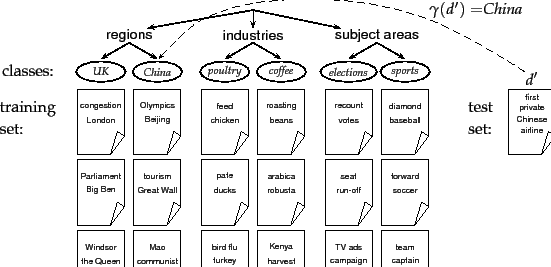
\includegraphics [scale=0.6] {hierarchy}
	\caption{Classes, training set, and test set in text classification.} 
	\label{img:hierarchy}  
\end{figure}


\section{A short review of existing mathematical models, which can be used to solve the classification problem} \label{sect1_3}

\begin{figure}[ht] 
	\center
	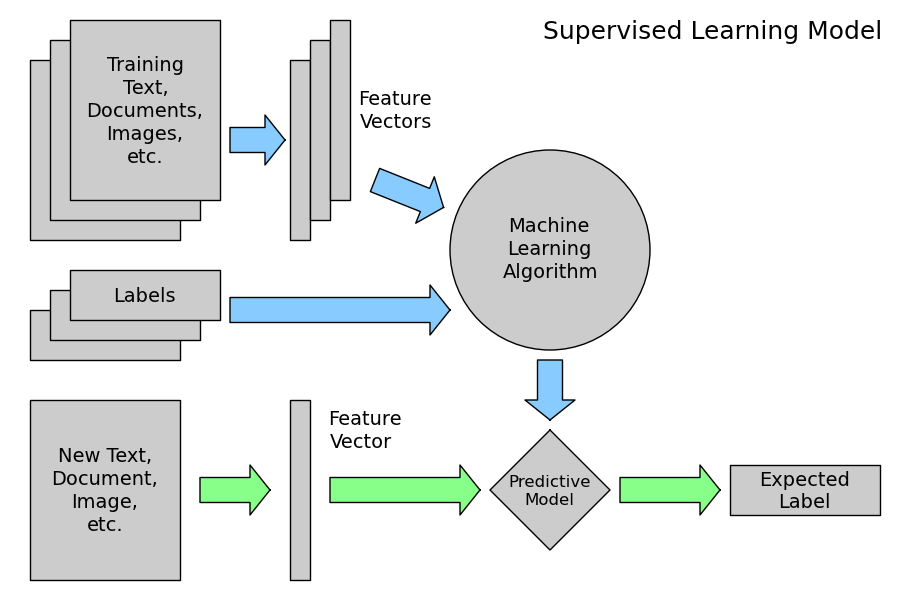
\includegraphics [scale=0.6] {work_flow}
	\caption{Supervised learning workflow.} 
	\label{img:supervised_learning_work_flow}  
\end{figure}

Supervised learning is the machine learning task of inferring a function from labelled training data. The training data consist of a set of training examples. Between inputs and reference outputs there may be some dependence, but it is unknown. On the basis of these data, it is necessary to restore the dependence. In order to measure the accuracy, a quality function can be introduced.\cite[p.7]{foundationsml} The diagram of the supervised learning process is presented in Figure ~\ref{img:supervised_learning_work_flow} 
\\

\noindent Here are some of the most important supervised learning algorithms:
\begin{enumerate}
	\item Naive Bayes .\cite{NB1}.\cite{NB2}
	%\item k-Nearest Neighbors
	\item Logistic Regression .\cite{LR}
	\item Support Vector Machines (SVMs) .\cite{svm}
	\item Decision Trees and Random Forests .\cite{manning}
	\item Neural networks .\cite{manning}
\end{enumerate}


\section{Model evaluation and validation} \label{sect1_4}
Machine learning pipeline is not finished with a model evaluation. We want to estimate correctly future data by using special techniques and metrics that are suitable for a particular task.

Now let us find out what validation is for?
\begin{enumerate}
	\item Validation helps to evaluate model performance, its quality, its ability to generalise.
	\item Validation can be used to select the best model to perform on unseen data.
	\item Overfitting of the model leads to the inconsistent and poor performance of the model on future data.
\end{enumerate}

To better understand each point we need to examine it more deeply.

\subsection{Model Evaluation Applications}
Very important property of learning models is Generalization performance. In general we want to estimate the predictive performance of our model on future data.  Therefore, it is necessary to use special techniques and metrics that are suitable for a particular task to track the performance of our models. 

When we have a set of candidate models model selection helps us to increase the predictive performance by tweaking the learning algorithm and selecting the best performing model from a given hypothesis space.
 
Before machine learning engineers find the best model, they make a bunch of experiments. Running a learning algorithm over a training dataset with different hyperparameter settings and various features will result in different models. The final goal is to select the best one from the set, ranking their performances against each other.

Algorithm selection - in most cases we deal with many algorithms to find the best one under the given circumstances. Therefore, we naturally need to compare different algorithms to each other, often regarding predictive and computational performance.
Nevertheless, these three sub-tasks have some similarities. When we want to estimate the performance of a model, they all require different approaches.


\subsection{Model Evaluation Techniques}
Holdout method (simple train/test split)
The holdout method is the most straightforward model evaluation technique. We take our labelled dataset and split it randomly into two parts: a training set and a test set.Then, we fit a model to the training data and predict the labels of the test set. And the fraction of correct predictions reflects our estimate of the prediction.

\begin{figure}[h!] 
	\center
	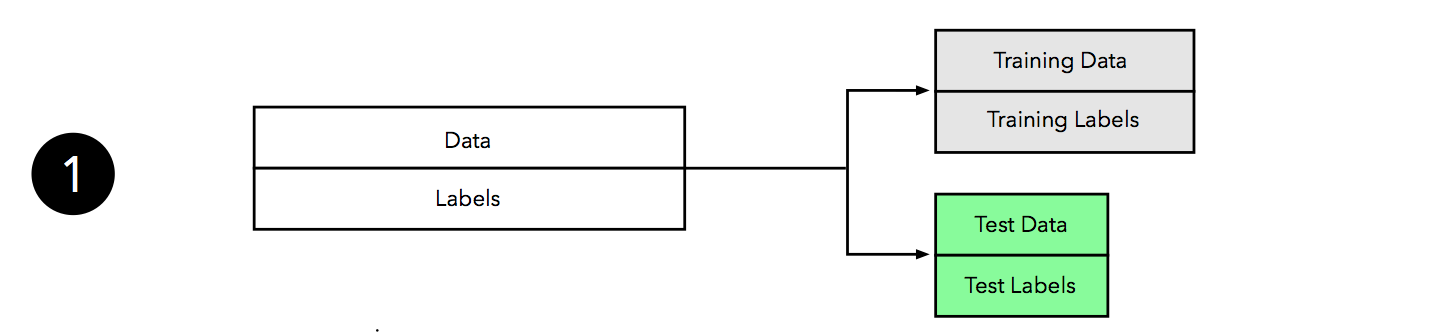
\includegraphics [scale=1] {eval1}
	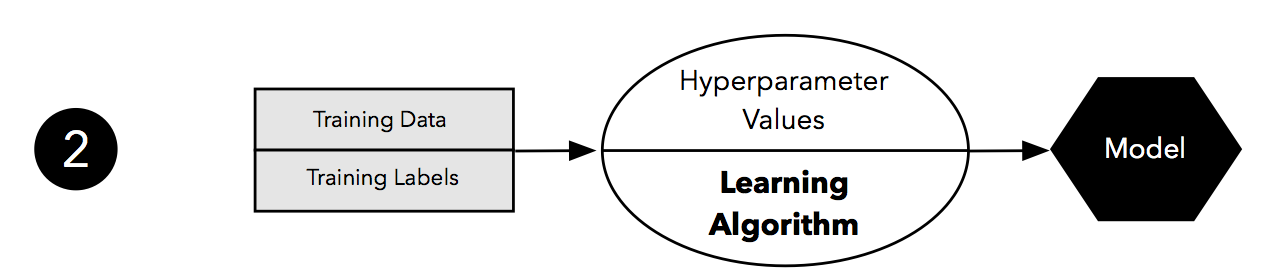
\includegraphics [scale=1] {eval2}
	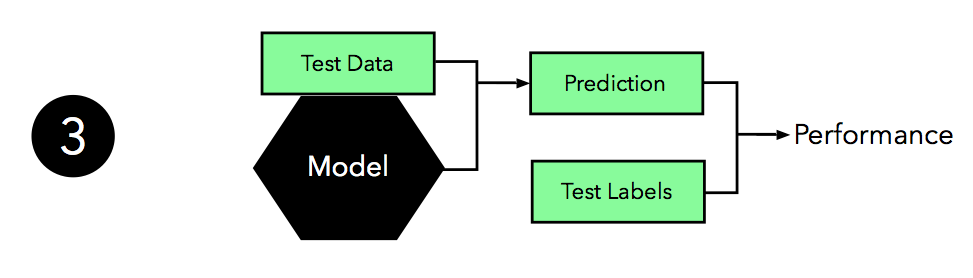
\includegraphics [scale=1] {eval3}
	\caption{Holdout method} 
	\label{img:eval3}  
\end{figure}

We don’t want to train and evaluate our model on the same training dataset, because it will lead to overfitting - the model will simply memorise the training data, and it will generalise wrong to unseen data. \cite{model_evaluation}


\section{Classification metrics}

Classification problems are probably the most common type of ML problem, and therefore many metrics can be used to evaluate predictions of these problems. The most frequently used metrics for classification problems are:

\begin{enumerate}
	\item Accuracy \ref{accuracy} \\
	Accuracy simply measures what percent of your predictions was correct. It's the ratio between the number of correct predictions and the total number of predictions.
	
	\begin{equation}
	\label{accuracy}
	accuracy = {\frac{correct}{predictions}}
	\end{equation}
\begin{doublespacing}
\end{doublespacing}
	
	Accuracy measures merely what percent of forecasts were correct. Accuracy is also the most misused metric. It is actually only suitable when there is an *equal number of observations in each class* (which is rarely the case) and that all *predictions and prediction errors are equally important, which is often not the case.
	
	\item Confusion Matrix 1.4 \\
	The confusion matrix is a handy presentation of the accuracy of a model with 2 or more classes. The table presents predictions on the x-axis and accuracy outcomes on the y-axis. The cells of the table are the number of predictions made by a machine learning algorithm.
	
	\newcommand\MyBox[2]{
		\fbox{\lower0.75cm
			\vbox to 1.7cm{\vfil
				\hbox to 2.2cm{\hfil\parbox{1.4cm}{#1\\#2}\hfil}
				\vfil}%
		}%
	}
	
	\noindent
	\begin{figure}[ht] 
		\center
		\label{img:CM} 
		\renewcommand\arraystretch{1.5}
		\setlength\tabcolsep{0pt}
		\begin{tabular}
			{c >{\bfseries}r @{\hspace{0.8em}}c @{\hspace{0.4em}}c @{\hspace{0.7em}}l}
			\multirow{10}{*}{\parbox{1.1cm}{\bfseries\raggedleft actual\\ value}} & 
			& \multicolumn{2}{c}{\bfseries Prediction outcome} & \\
			& & \bfseries p & \bfseries n & \bfseries total \\
			& p$'$ & \MyBox{True}{Positive} & \MyBox{False}{Negative} & P$'$ \\[2.4em]
			& n$'$ & \MyBox{False}{Positive} & \MyBox{True}{Negative} & N$'$ \\
			& total & P & N &
		\end{tabular}	
		\caption{Confusion matrix} 
		 
	\end{figure}
	
	Confusion matrix allows one to compute various classification metrics.
	
	\item Precision \ref{precision} and Recall \ref{recall}\\
	Precision and recall are two metrics. But they are often used together.
	Precision answers the question: What percent of positive predictions was correct?
	
	\begin{equation}
	\label{precision}
	precision = {\frac{\#\ true\ positive}{\#\ true\ positive + \#\ false\ positive}}
	\end{equation}
\begin{doublespacing}
\end{doublespacing}
	
	Recall answers the question: What percent of the positive cases did you catch?
	
	\begin{equation}
	\label{recall}
	recall = {\frac{\#\ true\ positive}{\#\ true\ positive + \#\ false\ negative}}
	\end{equation}
\begin{doublespacing}
\end{doublespacing}
	
	\item F1-score \ref{f1}\\
	The F1-score (sometimes known as the balanced F-beta score) is a single metric that combines both precision and recall via their harmonic mean:
	
	\begin{equation}
	\label{f1}
	F_1 = 2 {\frac{precision * recall}{precision + recall}}
	\end{equation}
\begin{doublespacing}
\end{doublespacing}
	
	Unlike the arithmetic mean, the harmonic mean tends toward the smaller of the two elements. Hence the F1 score will be small if either precision or recall is small.
\end{enumerate}

\section{Summary of the section}

In the first section the relevance of the problem and the main concepts associated with it are considered, namely, classification, its formation, intellectual analysis. It is a review of the main methods and algorithms of classification and criteria for its management.

Since it is important to investigate not only the ways to classify texts, but also attempts to understand main features, which had the highest importance. It is important to study the theory of how to represent textual information before applying algorithms. Then, from the examined algorithms, the deep neural networks will be used. 

With the criterion for further work, the top-5 accuracy and F1-score curve were selected.
           % Глава 1
\chapter{Mathematical models and algorithms for text classification} \label{chapt2}

\section{Words representations} \label{sect2_1}


In supervised learning domain, to perform classification tasks, our goal is usually to find a parametrized model, best in its class: 

\begin{equation}
\label{eq:equation1}
A(X, \hat{w}): A(X, \hat{w}) \simeq f(X) \Leftrightarrow A(X, \hat{w}) = \operatorname*{arg\,min}_w \left\|A(X, w) - f(X)\right\|
\end{equation}

Where $X \in R^{ n\times m}$ - feature matrix ($n$ observations with $m$ features), $w \in R^{m}$ - vector of model parameters, $\hat{w}$ - "best" model parameters. However, as a candidate for X - all that we have is raw text input, algorithms can not use it as it is. In order to apply machine learning on textual data, firstly content should be transformed into the specific numerical format, other words it is necessary to form feature vectors. In Natural Language Processing automated feature extraction may be achieved in many ways. I will cover the most frequently used in the modern practices.

\subsection{Bag-of-Words Approach} \label{subsect2_1_1}

Bag-of-words is an unordered set of words, with their exact position ignored.\cite[p.641]{jurafsky}, 


\noindent In bag-of-words approach we work under the following assumptions:
\begin{itemize}
	\item The text can be analyzed without taking into account the word/token order.
	\item It is only necessary to know which words/tokens of the text consists of and how many times.
\end{itemize}

Formally, there is a collection of texts $T_1, T_2, ... , T_n$. Unique tokens $w_1, w_2, ..., w_m$ are extracted to form a dictionary. Thus, each text $T_i$ is represented by feature vector $F_j = \{x_{ij},\ j \in [1,m]\}$, where $x_{ij}$ corresponds to number of occurrences of word $w_j$ in text $T_i$.

Example:
Our corpus is represented by 2 texts:
["The sun is yellow", "The sky is blue"]

Our tokens are simple unigrams, therefore there are 6 unique words: {the, sun, is, yellow, sky, blue}. Then, given corpus is mapped to feature vectors:
$T_1=(1,1,1,1,0,0)$, $T_2=(1,0,1,0,1,1)$ 

\begin{table} [htbp]
	\centering
	\parbox{15cm}{\caption{Feature vector}\label{Ts0Sib_}}
	%  \begin{center}
	\begin{tabular}{| p{1cm} || p{1cm} | p{1cm} | p{1cm} | p{2cm} | p{1cm} | p{1cm}l |}
		\hline
		\hline
		Text & \centering the  & \centering sun  & \centering is  &\centering yellow &\centering sky  & \centering  blue & \\
		\hline
		$T_{1}$ &\centering  1   &\centering  1  &\centering  1   &\centering  1 &\centering  0 &\centering 0 &   \\
		$T_{2}$ &\centering  1   &\centering  0  &\centering  1   &\centering  0 &\centering  1 &\centering 1 &   \\
		\hline
		\hline
	\end{tabular}
	%  \end{center}
\end{table}

\noindent Benefits:
\begin{itemize}
	\item Despite its simplicity, it demonstrates good results.
	\item Fast preprocessing.
	\item Built-in in many scientific/NLP libraries
\end{itemize}

\noindent Drawbacks:
\begin{itemize}
	\item Huge corpus usually leads to huge vocabulary size.
	\item Not memory-efficient: if we have corpus with 20 thousand texts then this textual corpus might spawn a dictionary with around 100 thousand elements. Thus, storing feature vectors as an array of type int32 would require 20000 x 100000 x 4 bytes $~$ 8GB in RAM.
	\item A bag of words is an orderless representation: throwing out spatial relationships between features leads to the fact that simplified model cannot let us distinguish between sentences, built from the same words, while having opposite meanings:"These paintings don't feel like ugly - buy them!" (positive) and "These paintings feel like ugly - don't buy them!" (negative) 
\end{itemize}

In order to capture dependencies between words N-grams technique can be used. N-gram is a sequence of $N$ basic tokens, which can be defined in different ways. 


Word n-grams - catch more semantics:
	\begin{itemize}
		\item unigrams: "The sun is yellow." $\rightarrow$ ['The', 'sun', 'is' ...]
		\item bigrams: "The sun is yellow." $\rightarrow$
		['The sun', 'sun is' ...]
		\item 3-grams: "The sun is yellow." $\rightarrow$
		['The sun is ', 'sun is yellow']
	\end{itemize}


In TF-IDF approach (term frequency - inverse document frequency), in addition to usual BoW-model, the following augmentation is made:

\subsection{TF-IDF  Approach} \label{subsect2_1_2}
Instead of just counting up the overlapping words, the algorithms apply a weight to each overlapping word. The TF weight measures how many times the word occurs in a particular document while the IDF weight measures how many different documents a word occurs in and is thus a way of discounting function words. Since function words like the, of, etc., occur in many documents, their IDF is very low, while the TF of the content words is high.\cite[p.647]{jurafsky} Formally it can be defined as: 



\begin{equation}
\label{eq:equation2_2}
\begin{cases} TF(w,T)=n_{Tw} \\ IDF(w, T)= log{\frac{N}{n_{w}}}\end{cases} \implies
TF\text{-}IDF(w, T) = n_{Tw}\ log{\frac{N}{n_{w}}} \ \ \ \ \forall w \in W
\end{equation}
\hfill \break 
where $T$ corresponds to current document (text), \hfill \break 
$w$ - selected word in document T, \hfill \break
$n_{Tw}$ - number of occurences of $w$ in text $T$, \hfill \break
$n_{w}$ - number of documents, containing word $w$, \hfill \break
$N$ - total number of documents in a corpus.

\begin{equation}
\label{eq:equation2_3}
\lim_{n_{w} \to N} {TF\text{-}IDF(w, T)} = 0
\end{equation}

\subsection{Embeddings} \label{subsect2_1_3}

Core idea: the meaning of a word is	given by the words	that frequently	appear	close-by. The fundamental ideas are stated in the following publications \cite{embeddings_1}, \cite{embeddings_2}. 



1. Skip-gram model

\noindent I would like to start the consideration of embeddings methods with the key definitions of softmax~\ref{eq:equation2_4}  and sigmoid~\ref{eq:equation2_5} functions,

\begin{equation}
\label{eq:equation2_4}
\textrm{softmax}({\bf x})_{i} = \frac{e^{x_{i}}}{\sum_{j=1}{e^{x_{j}}}}
\end{equation}

\begin{equation}
\label{eq:equation2_5}
\textrm{sigmoid} = \sigma(z) = \frac{1}{1 + e^{-z}}.
\end{equation}

\noindent The gradient of sigmoid function is follows:

\begin{equation}
\label{eq:equation2_6}
\sigma^{\prime}(z) = \sigma(z)(1 - \sigma(z))
\end{equation}


\begin{figure}[ht] 
	\center
	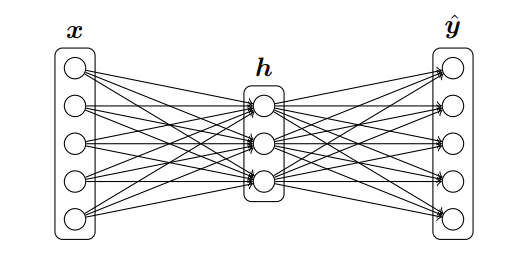
\includegraphics [scale=0.5] {FCNN}
	\caption{Neural Network} 
	\label{img:FCNN}  
\end{figure}

\noindent where $x$ is one-hot input vector, $h$ - hidden layer, y is the one-hot label vector, and ŷ is the predicted probability vector for all classes.The neural network Figure \ref{img:FCNN} employs sigmoid activation function for the hidden layer, and softmax for the output layer and cross entropy cost ~\ref{eq:equation2_7} is used.

\begin{equation}
\label{eq:equation2_8}
\textrm{CE}({\bf y},{\bf\hat{y}}) = -\sum_{i}{y_{i}\log{\hat{y_{i}}}}
\end{equation}

Now, we will compute the gradient of cross entropy:

\begin{equation}
\label{eq:equation_CE_2}
\frac{\partial(\textrm{CE})}{\partial{\hat{y}_{i}}} = -\frac{y_{j}}{\hat{y}_{i}}
\end{equation}
That leads, 

\begin{equation}
\frac{\partial(\textrm{CE})}{\partial{\theta_{k}}} =  \frac{\partial(\textrm{CE})}{\partial{\hat{y}_{i}}}\frac{\partial{\hat{y}_{i}}}{\partial{\theta_{k}}} 
=-\frac{y_{j}}{\hat{y}_{i}}\frac{\partial{\hat{y}_{i}}}{\partial{\theta_{k}}}
\end{equation}

Function $softmax$ for i-th output depends not only on its $\theta_{i}$, but also on all other $\theta_{k}$, the sum of which lies in the denominator of the formula for direct passage through the network. Therefore, the formula for back propagation "splits" into two: the partial derivative with respect to $\theta_{i}$ and $\theta_{k}$:

\begin{equation}
\begin{multlined}
\label{eq:equation_CE_3}
\frac{\partial{\hat{y}_{i}}}{\partial{\theta_{i}}} =  \frac{\partial}{\partial{\theta_{i}}}\left( \frac{e^{\theta_{i}}}{\sum_{j=1}{e^{\theta_{j}}}}\right) =\\
= \frac{e^{\theta_{i}}}{\sum_{j=1}{e^{\theta_{j}}}} - \left(\frac{e^{\theta_{i}}}{\sum_{j=1}{e^{\theta_{j}}}}\right)^{2} = \\
= \hat{y}_{i}\cdot(1 - \hat{y}_{i})
\end{multlined}
\end{equation}

and (where $i\neq k$),

\begin{equation}
\label{eq:equation_CE_4}
\begin{multlined}
\frac{\partial{\hat{y}_{i}}}{\partial{\theta_{k}}} =  \frac{\partial}{\partial{\theta_{k}}}\left( \frac{e^{\theta_{i}}}{\sum_{j=1}{e^{\theta_{j}}}}\right) = \\
=-\left(\frac{e^{\theta_{i}}e^{\theta_{k}}}{\sum_{j=1}{e^{\theta_{j}}}}\right)
= - \hat{y}_{i}\hat{y}_{k}
\end{multlined}
\end{equation}

After combination of equations~\ref{eq:equation_CE_2},~\ref{eq:equation_CE_3},~\ref{eq:equation_CE_4}, 

\begin{equation}
\label{eq:CE_gradient}
\frac{\partial(\textrm{CE})}{\partial{\theta_{k}}} = \begin{cases}
-y_{j}(1 - \hat{y}_{k})&\text{ for }i=k \\
y_{j}\hat{y}_{k}&\text{ for }i\neq k
\end{cases}
\end{equation}

$y_{j}$ should be non-zero, $k=j$ and $y_{j}=1$, leads to,

\begin{equation}
\label{eq:equation_CE_5}
\frac{\partial(\textrm{CE})}{\partial{\theta_{j}}} = \begin{cases}
(\hat{y}_{j} - 1)&\text{ for }i=j \\
\hat{y}_{j}&\text{ for }i\neq j
\end{cases}
\end{equation}

Which is equivalent to,

\begin{equation}
\frac{\partial(\textrm{CE})}{\partial{\boldsymbol\theta}} = \bf{\hat{y}} - \bf{y}
\end{equation}

\noindent Forward propagation is as follows:
\begin{equation}
{\bf h} = \textrm{sigmoid}({\bf x\textrm{W}_{1} + b_{1}}) 
\end{equation}

\begin{equation}
\label{eq:equation2_7}
{\bf \hat{y}} = \textrm{softmax}({\bf h\textrm{W}_{2} + b_{2})}
\end{equation}

\noindent where $\bf{\textrm{W}}_i$ and $\bf{b}_{i}$ ($i\in\{1,2\}$) are
the weights and biases, respectively of the two layers.
\indent To optimize weights for each layer of neural network a back propagation algorithm is used. Therefore, it is necessary to calculate the gradients for each layer.
  
\noindent In order to simplify the notation used to solve the problem, define the following terms:
\begin{equation}
\label{eq:equation2_10}
\begin{multlined}
		 {\bf z}_{1}\equiv \quad{\bf x\textrm{W}_{1} + b_{1}} \\
		{\bf z}_{2}\equiv \quad{\bf h\textrm{W}_{2} + b_{2}}
\end{multlined}
\end{equation}

Starting with the results from ~\ref{eq:equation2_8}:

\begin{equation}
\frac{\partial{J}}{\partial{\bf z}_{2}} = \bf{\hat{y}} - \bf{y}
\end{equation}

and

\begin{equation}
\label{eq:equation2_11}
\frac{\partial{\bf z}_{2}}{\partial{{\bf h}}} = {\bf \textrm{W}^{\top}_{2}}
\end{equation}

Sigmoid ($\sigma$) derivative ~\ref{eq:equation2_6}:

\begin{equation}
\frac{\partial{{\bf h}}}{\partial{{\bf z}_{1}}}\equiv\sigma^{\prime}(z_{1})
\end{equation}

Combining these, and using $\cdot$ to denote element-wise product:

\begin{equation}
\frac{\partial{J}}{\partial{z_{i}}} = (\bf{\hat{y}} - \bf{y}){\bf \textrm{W}^{\top}_{2}}\cdot\sigma^{\prime}(z_{1})
\end{equation}

Finally, using the results from Equation~\ref{eq:equation2_11}:

\begin{equation}
\frac{\partial{J}}{\partial{{\bf W}^{(1)}}} = (\bf{\hat{y}} - \bf{y}){\bf \textrm{W}^{\top}_{2}}\cdot\sigma^{\prime}(z_{1})\cdot{\bf \textrm{X}^{\top}}
\end{equation}  

\begin{equation}
\frac{\partial{J}}{\partial{{\bf W}^{(2)}}} = (\bf{\hat{y}} - \bf{y}){\bf \textrm{h}^{\top}}
\end{equation}  

We have everything to update our weights: 

%\clearpage
Now, turn definitely to skip-gram model shown in Figure ~\ref{img:skip_gram_model}\cite{embeddings_2}:
\begin{figure}[H] 
	\center
	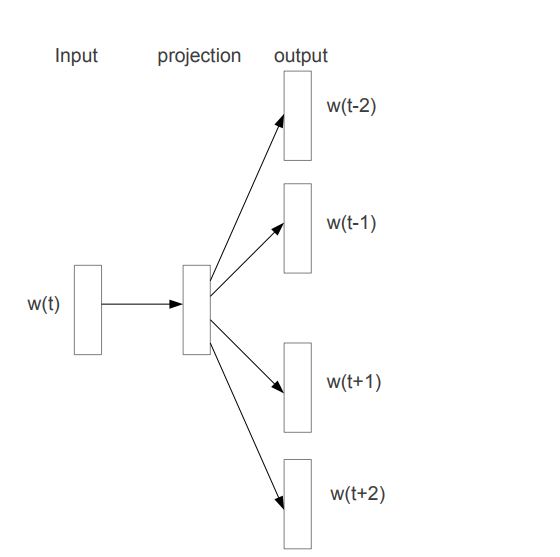
\includegraphics [scale=0.5] {skip_gram_model}
	\caption{The Skip-gram model architecture.} 
	\label{img:skip_gram_model}  
\end{figure}



\noindent Now, let`s transfer knowledge from above to our skip-gram model.    
We have a word vector ${\boldsymbol v}_{c}$ corresponding to the center word $c$ for
\texttt{skip-gram}, and word prediction is made with the \texttt{softmax} function: 

\begin{equation}
{\hat{\boldsymbol y}}_{\boldsymbol o} = p(~{\boldsymbol o} \mid {\boldsymbol c}~) = \frac{\exp{({\boldsymbol u}^{\top}_{o}{\boldsymbol v}_{c})}}{\sum^{\vert{W}\vert}_{j=1}\exp{({\boldsymbol u}^{\top}_{j}{\boldsymbol v}_{c})}}
\end{equation}

where $w$ denotes the $w$-th word and ${\boldsymbol u}_{w}$ ($w=1,...,\vert\textrm{W}\vert$)  are the `output' word vectors for all words in the vocabulary. Cross entropy cost is applied to this prediction and word $o$ is the expected word (the $o$-th element of the one-hot label vector is one). ${\boldsymbol U} = [ {\boldsymbol u}_{1}, {\boldsymbol u}_{2},...,{\boldsymbol u}_{\vert\textrm{W}\vert}]$ is the matrix of all the output vectors. 

Applying cross-entropy cost to the softmax probability defined above:

\begin{equation}
J =-\log{p} = - {\boldsymbol u}_{o}^{\top}{\boldsymbol v}_{c} + \log\sum^{\vert{V}\vert}_{j=1}\exp{({\boldsymbol u}_{j}^{\top}{\boldsymbol v}_{c})}
\end{equation}

Let $z_{j}={\boldsymbol u}_{j}^{\top}{\boldsymbol v}_{c}$, and $\delta^{i}_{j}$ ~\ref{eq:indicator} be the indicator function, then

\begin{equation}
\label{eq:indicator}
\delta^{i}_{j} =  
	\begin{cases}
	1, &\text{ for }i=j \\
	0, &\text{ for }i\neq j
	\end{cases}
\end{equation}


\begin{equation}
\frac{\partial J}{\partial{z_{k}}} = - \delta^{i}_{k} + \frac{\exp{({\boldsymbol u}_{i}^{\top}{\boldsymbol v}_{c})}}{\sum^{\vert{V}\vert}_{j=1}\exp{({\boldsymbol u}_{j}^{\top}{\boldsymbol v}_{c})}}
\end{equation}

Now, using the chain rule, we can calculate,

\begin{equation}
	\begin{multlined}
	\frac{\partial J}{\partial{{\boldsymbol v}_{c}}} =  \frac{\partial J}{\partial{{\boldsymbol z}}}\frac{\partial{{\boldsymbol z}}}{\partial{{\boldsymbol v}_{c}}} =\\
	= \sum^{\vert{V}\vert}_{j=1}{\boldsymbol u}_{j}^{\top}\left(\frac{e^{z_{j}}}{\sum^{\vert{V}\vert}_{k=1}e^{z_{k}}} -  1\right) =\\
	= \sum^{\vert{V}\vert}_{k=1}{\boldsymbol P}({\boldsymbol u}_{j} \vert {\boldsymbol v}_{c} ){\boldsymbol u}_{j} - {\boldsymbol u}_{j}
	\end{multlined}
\end{equation}


\noindent For the `output' word vectors ${\boldsymbol u}_{w}$'s

\begin{equation}
	\begin{multlined}
	\frac{\partial J}{\partial{\boldsymbol u}_{j}} = \frac{\partial J}{\partial{{\boldsymbol z}}}\frac{\partial{{\boldsymbol z}}}{\partial{\boldsymbol u}_{j}} =\\
	= {\boldsymbol v}_{c}\left(\frac{\exp{({\boldsymbol u}^{\top}_{0}{\boldsymbol v}_{c})}}{\sum^{\vert{V}\vert}_{j=1}\exp{({\boldsymbol u}^{\top}_{j}{\boldsymbol v}_{c})}} - \delta^{0}_{j}\right)
	\end{multlined}
\end{equation}

\noindent We have calculated the gradient for one particular word, now we will generalize this to a number of words. We have a set of context words [$\texttt{word}_{c-\textbf{m}},...,\texttt{word}_{c-\textbf{1}},\texttt{word}_{c},\texttt{word}_{c+\textbf{1}},...,\texttt{word}_{c+\textbf{m}}$ ], where \textbf{m} is the context size. We denote the `input' and `output' word vectors for $\texttt{word}_{k}$ as ${\boldsymbol v}_{k}$ and ${\boldsymbol u}_{k}$ respectively for
convenience. \\

\noindent Also it is a good idea to use $F({\boldsymbol o}, {\boldsymbol v}_{c})$ (where ${\boldsymbol o}$ is the expected word) as a placeholder for $J({\boldsymbol o}, {\boldsymbol v}_{c}, ...)$ cost functions.

\noindent Then we can rewrite cost function as follows:

\begin{equation}
J =   \sum_{-m\le j\le m, j\neq0}F({\boldsymbol w}_{c+j}, {\boldsymbol v}_{c})
\end{equation}

where ${\boldsymbol w}_{c+j}$ refers to the word at the $j$-th index from the center.\\

The derivative of the loss has two terms, ${\boldsymbol w}_{c+j}$ and ${\boldsymbol v}_{c}$, which yields the following ~\cite{assignment1},

\begin{equation}
	\begin{multlined}
	\frac{\partial{J}}{\partial{\boldsymbol w}_{k}} = \\ =\frac{\partial}{\partial{\boldsymbol w}_{k}}\sum_{-m\le j\le m, j\neq0}F({\boldsymbol w}_{c+j}, {\boldsymbol v}_{c})= \\
	= \sum_{-m\le j\le m, j\neq0} \frac{\partial{F}}{\partial{\boldsymbol w}_{i+j}}\delta^{i+j}_{k}
	\end{multlined}
\end{equation}

and

\begin{equation}
\frac{\partial{J}}{\partial{\boldsymbol v}_{c}} = \sum_{-m\le j\le m, j\neq0} \frac{\partial{F}}{\partial{\boldsymbol v}_{c}}
\end{equation}

Now, we can update our weight using gradient descent algorithm:

\begin{equation}\\
	\begin{multlined}
	w^{new}_{k} = w^{old}_{k} - \eta \frac{\partial{J}}{\partial{w}_{k}} \\
	v^{new}_{c} = v^{old}_{c} - \eta \frac{\partial{J}}{\partial{v}_{c}}
	\end{multlined}
\end{equation}

where $\eta$ is a learning rate.

After training the skip-gram model, we take the hidden layer weight matrix that will represent our words in the multidimensional space. If we make projection into two- dimensional space, we can have the following Figure ~\ref{img:embed}:

\begin{figure}[ht] 
	\center
	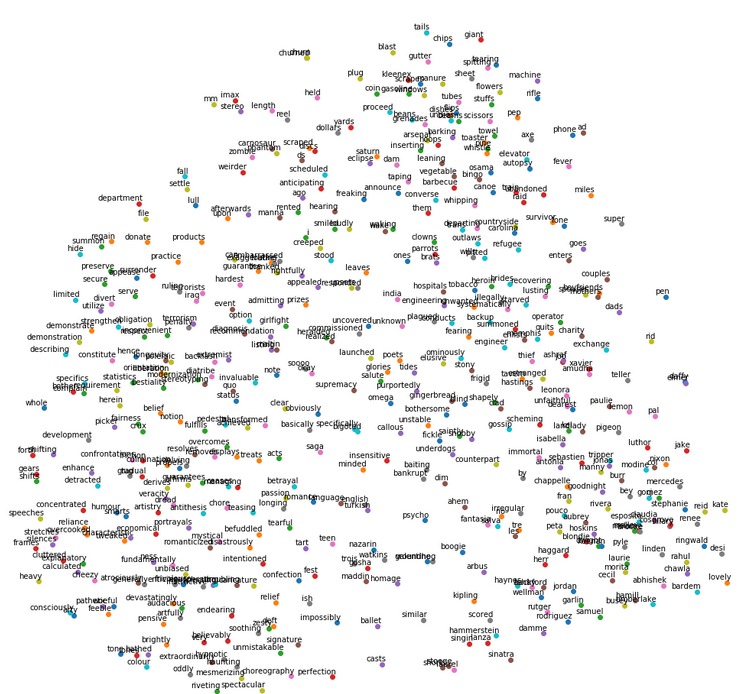
\includegraphics [scale=0.4] {embed}
	\caption{Words representation} 
	\label{img:embed}  
\end{figure}


However, this type of architecture, where for each output we need to compute separate $softmax$ function is very expensive in terms of computational resources and as a result time. Therefore, there are different ways to approximate the expensive $softmax$ function. The most famous of them are:

\begin{itemize}
	\item Negative Sampling technique
	\item Hierarchical Softmax
\end{itemize}
 

\noindent The only difference between Negative Sampling technique and the original model is that we introduce new loss function - negative sampling loss for the predicted vector ${\boldsymbol v}_{c}$, and 
the expected output word is ${\boldsymbol o}({\boldsymbol u}_{o})$. Assume that $K$ negative samples (words) are drawn, and they are ${\boldsymbol u}_{1},...,{\boldsymbol u}_{k}$, respectively for simplicity of notation ($k\in\{1,...,K\}$ and $o\notin\{1,...,K\}$). Again for a given word, ${\boldsymbol o}$, denote its output vector as ${\boldsymbol u}_{o}$. The negative sampling loss function in this case is,

\begin{equation}
J({\boldsymbol u}_{o}, {\boldsymbol v}_{c}, {\boldsymbol U}) = -\log(\sigma( {\boldsymbol u}^{\top}_{o}{\boldsymbol v}_{c})) - \sum^{K}_{k=1}\log(\sigma(- {\boldsymbol u}^{\top}_{k}{\boldsymbol v}_{c}))
\end{equation}

where $\sigma(\cdot)$ is the sigmoid function.\\
As it can be clearly seen, now we make calculations not on the whole vocabulary $V$, but only on the part of it, which is randomly generated each time. 

~\\ 
Hierarchical Softmax is an approximation which uses a binary tree to compute the necessary probability. 
This gives us a possibility to decompose calculating the probability of one word into a sequence of probability calculations. Balanced threes have a maximum depth of $log_2(|V|)$, which means that in the worst case we need to calculate $log_2(|V|)$ nodes to find the necessary probability of a certain word.  

Both methods enable us a possibility to significantly decrease the amount of time for computation.

2.CBOW model
This model is very similar to skip-gram, but CBOW predicts a target word from the bag of words context. From the practical point of view, skip-gram works well with a small amount of training data and represents well even rare words or phrases. CBOW is several times faster to train than the skip-gram and has slightly better accuracy for the frequent words. This model is shown in Figure ~\ref{img:CBOW}\cite{embeddings_2}:

\begin{figure}[ht] 
	\center
	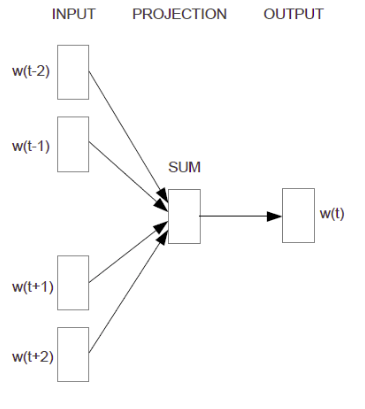
\includegraphics [scale=0.6] {CBOW}
	\caption{The CBOW model architecture.} 
	\label{img:CBOW}  
\end{figure}

\section{Deep learning algorithms for text classification}\label{sect2_2}

When people hear about NLP problems and neural networks in one context they probably think about Recurrent neural networks or their modification. 
However, recently some papers which apply CNN's to problems in Natural Language Processing were published and they got some interesting results \cite{CNN} \cite{Kalchbrenner}. In this section I will consider both CNN and RNN models and their modifications.


\subsection{Convolution Neural Networks}\label{sect2_2_1}  

\begin{figure}[ht] 
	\center
	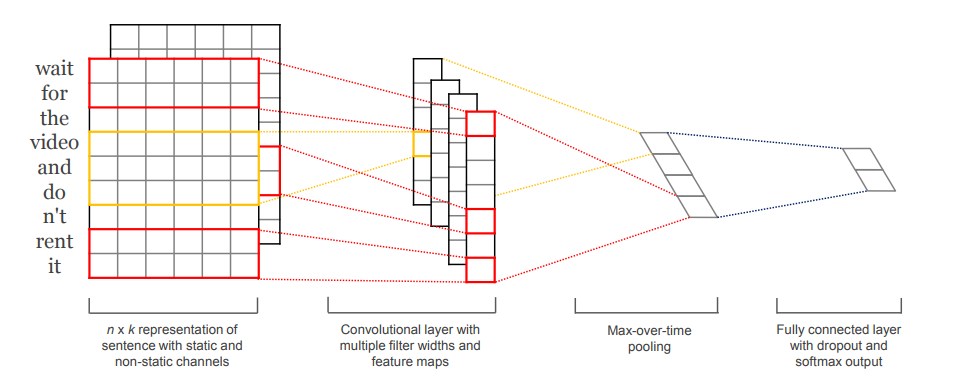
\includegraphics [scale=0.5] {CNN}
	\caption{Convolution Neural Networks architecture for text classification} 
	\label{img:CNN}  
\end{figure}

The model architecture, shown in Figure ~\ref{img:CNN} \cite{CNN}, is a variant of the CNN architecture. Let $x_i \in \mathbb{X}$ be the k-dimensional word vector corresponding to the i-th word in the sentence, a sentence of length n. In general, let $x_{i:i+j}$ refers to the concatenation of words $\{x_{i}, x_{i+1}, . . . , x_{i+j}\}$.\cite{CNN}


\subsubsection{Convolution}\label{sect2_2_1_1} 

\begin{figure}[ht] 
	\center
	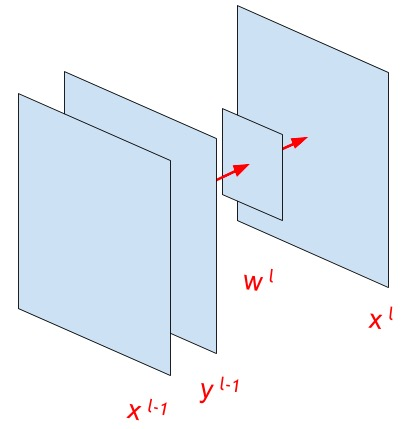
\includegraphics [scale=0.5] {convolution}
	\caption{Basic variables used in the convolution layer} 
	\label{img:convolution}  
\end{figure}

In the convolution neural network, a limited matrix of small weights is used in the convolution operation, which is moved along the entire processed layer, forming after each shift the activation signal for the neuron of the next layer with the same position. The same matrix of weights, called kernel, is used for different neurons of the output layer.  
The schema of this process is illustrated in the Figure ~\ref{img:convolution} \cite{CNN_habr}.

The following equation ~\ref{eq:convolution} describes the words above into mathematical way:

\begin{equation}
\label{eq:convolution}
x^l_{ij}=\sum_{a=-\infty}^{+\infty}\sum_{b=-\infty}^{+\infty}w^l_{ab}\cdot y^{l-1}_{(i\cdot s-a)(j\cdot s-b)}+b^l \qquad \forall i\in (0,...,N) \enspace \forall j\in (0,...,M) 
\end{equation}

where $i, j, a, b$ - indexes of elements in matrices, $s$ - step's size of convolution

\noindent The superscripts $l$ and $l-1$ are the indices of the network layers.\\
$x_{l-1}$ - the output of some previous function, or the input of the network \\
$y_{l-1}$ - $x_{l-1}$ after passing the activation function \\
$w_{l}$ - the convolution kernel \\
$b_{l}$ - bias or offset \\
$x_{l}$ - the result of the operation of convolution. That is, the operations which goe separately for each element $i,j$ of the matrix $x_{l}$, whose dimension is $(N, M)$.

The important moment which I should pay attention to is Central Core Element, because indexing of the elements takes place depending on the location of the central element. In fact, the central element determines the origin of the "coordinate axis" of the convolution kernel. 

\subsubsection{Activation functions}
\indent Activation function is a transformation which has a general view $y^l=f(x^l)$. I did not cover all existing activations functions, I chose only those which were used in the current model. 

1) ReLu \ref{eq:Relu}, \ref{img:Relu} - this activation function was used at Convolution layers. It has the following properties:


\begin{equation}
\label{eq:Relu}
f_{ReLU}=max(0,x)
\end{equation}

\begin{figure}[H] 
	\center
	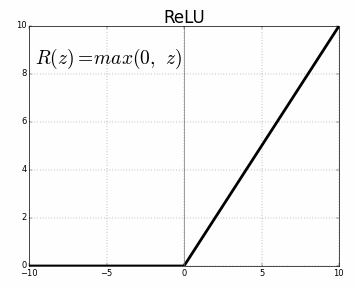
\includegraphics [scale=0.4] {Relu}
	\caption{ReLu activation function} 
	\label{img:Relu}  
\end{figure}


2) Softmax \ref{eq:equation2_4} - I deal with multi-class classification, therefore this activation was picked.


\subsubsection{Max pulling layer} 
\indent This layer allows one to highlight important features on the maps of features obtained from convolution layer, gives an invariance to find the object on the cards, and also reduces the dimensionality of the maps, speeding up the network time. It works in the following way Figure \ref{img:max_pulling}: we divide our features from convolution layer into disjoint $m \times n$ regions, and take the maximum feature activation over these regions. These new features can be used for classification.

\begin{figure}[ht] 
	\center
	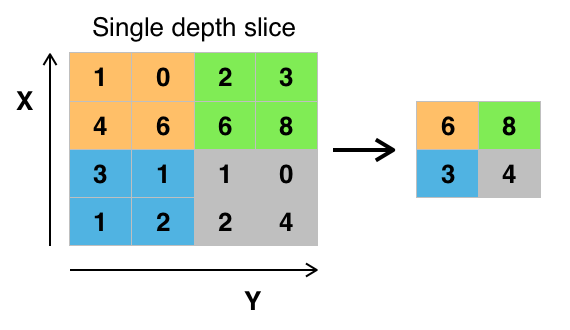
\includegraphics [scale=0.5]{max_pulling}
	\caption{Max pulling layer} 
	\label{img:max_pulling}  
\end{figure}


\subsubsection{Fully connected layer}
\indent After layers of the convolution and max pooling, we obtain a set of feature cards. We connect them into one vector and this vector will be fed into the fully connected network.
The Figure \ref{img:CNN_FNN_layer} describes this stage.

\begin{figure}[ht] 
	\center
	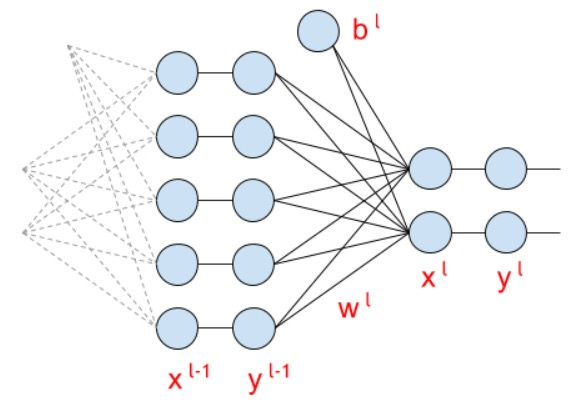
\includegraphics [scale=0.5] {CNN_FNN_layer}
	\caption{Fully connected layer of CNN} 
	\label{img:CNN_FNN_layer}  
\end{figure}

\begin{equation}
x^l_i=\sum_{k=0}^{m}w^l_{ki}y^{l-1}_k+b^l_i \qquad \forall i\in (0,...,n)
\end{equation}

in matrix representation:

\begin{equation}
	X^l=Y^{l-1}W^l+B^l_i 
\end{equation}

\noindent Loss function for the model is Cross Entropy \ref{eq:equation2_8} described above.

Now after all components of CNN are known, we need to optimize weights for each layer. Therefore, it is necessary to derive the formula for back propagation through the loss function. 

1) Hopefully, the gradient for loss function was already founded \ref{eq:equation_CE_3}, \ref{eq:equation_CE_4}, \ref{eq:CE_gradient}.
Therefore, we have the following equation \ref{eq:CNN_softmax_grad}: 

\begin{equation}
	\label{eq:CNN_softmax_grad}
	\begin{multlined}
	 \frac{\partial J}{\partial x^l_i} = \sum_{k=0}^{n} \frac{\partial J}{\partial y^l_k} \frac {\partial y^l_k} {\partial x^l_i} = \frac{\partial J}{\partial y^l_0} \frac {\partial y^l_0} {\partial x^l_i} + ... \\ + \frac{\partial J}{\partial y^l_1} \frac {\partial y^l_1} {\partial x^l_i} + ...
	 + \frac{\partial J}{\partial y^l_n} \frac {\partial y^l_n} {\partial x^l_i} \qquad \forall i \in (0,...n)
	\end{multlined}
\end{equation}

or 
\begin{equation}
\label{eq:CNN_softmax_grad_long}
	\begin{multlined}
	\begin{bmatrix} 
	&\frac{\partial J}{\partial x^{l}_{0}} &\frac{\partial J}{\partial x^{l}_{1}} & ... &\frac{\partial J}{\partial x^{l}_{n}} 
	\end{bmatrix} 
	= \\= \scriptsize 
	\begin{bmatrix} & (\frac{\partial J}{\partial y^{l}_{0}}\frac{\partial y^{l}_{0}}{\partial x^{l}_{0}}+\frac{\partial J}{\partial y^{l}_{1}}\frac{\partial y^{l}_{1}}{\partial x^{l}_{0}}+\ldots+\frac{\partial J}{\partial y^{l}_{n}}\frac{\partial y^{l}_{n}}{\partial x^{l}_{0}}) & (\frac{\partial J}{\partial y^{l}_{0}}\frac{\partial y^{l}_{0}}{\partial x^{l}_{1}}+\frac{\partial J}{\partial y^{l}_{1}}\frac{\partial y^{l}_{1}}{\partial x^{l}_{1}}+\ldots+\frac{\partial J}{\partial y^{l}_{n}}\frac{\partial y^{l}_{n}}{\partial x^{l}_{1}}) & ... & (\frac{\partial J}{\partial y^{l}_{0}}\frac{\partial y^{l}_{0}}{\partial x^{l}_{n}}+\frac{\partial J}{\partial y^{l}_{1}}\frac{\partial y^{l}_{1}}{\partial x^{l}_{n}}+\ldots+\frac{\partial J}{\partial y^{l}_{n}}\frac{\partial y^{l}_{n}}{\partial x^{l}_{n}}) 
	\end{bmatrix} \\= 
	\begin{bmatrix} &\frac{\partial J}{\partial y^{l}_{0}} &\frac{\partial J}{\partial y^{l}_{1}} & ... &\frac{\partial J}{\partial y^{l}_{n}} 
	\end{bmatrix} 
	\begin{bmatrix} &\frac{\partial y^{l}_{0}}{\partial x^{l}_{0}} &\frac{\partial y^{l}_{0}}{\partial x^{l}_{1}}&...&\frac{\partial y^{l}_{0}}{\partial x^{l}_{n}}\\ &\frac{\partial y^{l}_{1}}{\partial x^{l}_{0}} &\frac{\partial y^{l}_{1}}{\partial x^{l}_{1}}&...&\frac{\partial y^{l}_{1}}{\partial x^{l}_{n}}\\ &...&...&...&...\\ &\frac{\partial y^{l}_{n}}{\partial x^{l}_{0}} &\frac{\partial y^{l}_{n}}{\partial x^{l}_{1}}&...&\frac{\partial y^{l}_{n}}{\partial x^{l}_{n}}\\ 
	\end{bmatrix}
	\end{multlined}
\end{equation}

Next, we should update the weights of fully connected layer matrix $w^l$. 
\begin{equation}
\frac{\partial J}{\partial w^l} = \dfrac{\partial J}{\partial y^l}\dfrac{\partial y^l}{\partial x^l}\dfrac{\partial x^l}{\partial w^l} = \delta^l \cdot \dfrac{\partial x^l}{\partial w^l} = \left(y^{l-1} \right)^T \cdot \delta^l    
\end{equation}

and $b^l$

\begin{equation}
\frac{\partial J}{\partial b^l}=\delta^l
\end{equation}

Equation for back propagation through $y^{l-1}$

\begin{equation}
 \dfrac{\partial J}{\partial y^{l-1}} = \delta^l \cdot \dfrac{\partial x^l}{\partial y^{l-1}}= \delta^l \cdot (w^l)^{T} = \delta^{l-1}
\end{equation} 

After this, we need to go with backprop through the layer of max pulling Figure \ref{img:backprog_max_pulling}.
The error "passes" only through those values of the original matrix, which were chosen by the maximum at the step of the max puling. The remaining error values for the matrix will be zero. 

\begin{figure}[ht] 
	\center
	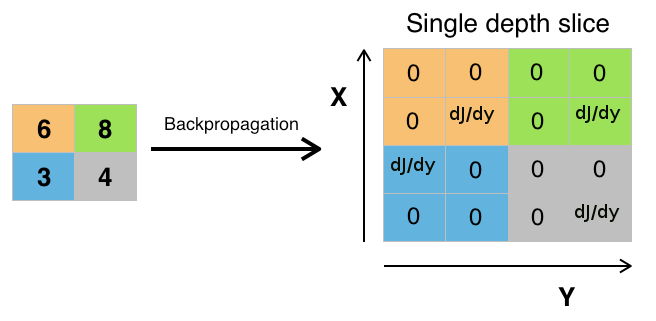
\includegraphics [scale=0.5]{backprog_max_pulling}
	\caption{Back propagation through max pulling layer} 
	\label{img:backprog_max_pulling}  
\end{figure}

It is necessary to derive weights update for kernel Figure \ref{img:conv_grad}. 

\begin{figure}[ht] 
	\center
	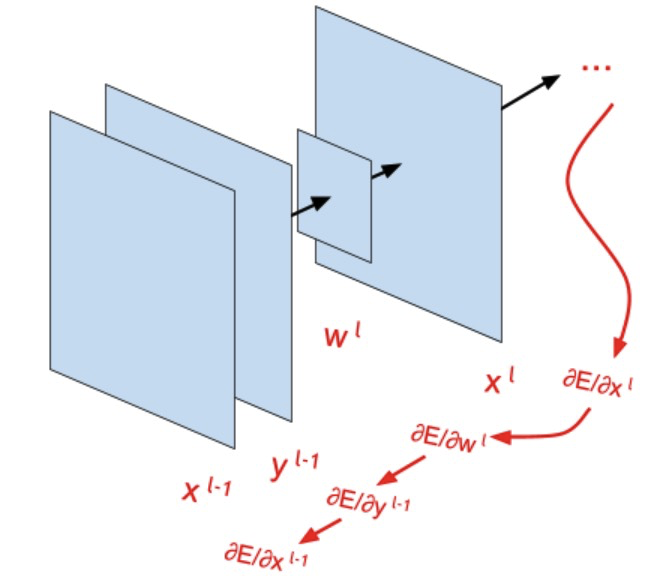
\includegraphics [scale=0.4]{conv_grad}
	\caption{Back propagation through convolution layer} 
	\label{img:conv_grad}  
\end{figure}

\begin{equation}
\begin{array}{rcl} 
\dfrac{\partial J}{\partial w^l_{ab}}&=&\sum_{i}\sum_{j} \dfrac{\partial J}{\partial y^l_{ij}}\dfrac{\partial y^l_{ij}}{\partial x^l_{ij}}\dfrac{\partial x^l_{ij}}{\partial w^l_{ab}}\\ &=&^{(1)}\sum_{i}\sum_{j} \dfrac{\partial J}{\partial y^l_{ij}}\dfrac{\partial y^l_{ij}}{\partial x^l_{ij}}\cdot \dfrac{\partial \left( \sum_{a'=-\infty}^{+\infty} \sum_{b'=-\infty}^{+\infty} w^l_{a'b'} \cdot y^{l-1}_{(is-a')(js-b')}+b^l \right)}{\partial w^l_{ab}}\\ &=&^{(2)}\sum_{i}\sum_{j} \dfrac{\partial J}{\partial y^l_{ij}}\dfrac{\partial y^l_{ij}}{\partial x^l_{ij}} \cdot y^{l-1}_{(is-a)(js-b)} \\ &&\forall a \in (-\infty,...,+\infty) \enspace \forall b \in (-\infty,...,+\infty) 
\end{array}\\
\end{equation}

all partial derivatives in the numerator, except those for which $a^{'}= a, b^{'} = b$, will be zero. 

~\\
Derivation of the gradient for the bias element. 
\begin{equation}
 \dfrac{\partial J}{\partial b^l} = \sum_{i}\sum_{j} \dfrac{\partial J}{\partial y^l_{ij}}\dfrac{\partial y^l_{ij}}{\partial x^l_{ij}}\dfrac{\partial x^l_{ij}}{\partial b^l} = \sum_{i}\sum_{j} \dfrac{\partial J}{\partial y^l_{ij}}\dfrac{\partial y^l_{ij}}{\partial x^l_{ij}} 
\end{equation}

\noindent The derivation of the equation for backprop through the convolution layer.

\begin{equation}
\frac{\partial J}{\partial y^{l-1}_{ij}}= \sum_{i'}\sum_{j'} \frac{\partial J}{\partial y^l_{i'j'}}\frac{\partial y^l_{i'j'}}{\partial x^l_{i'j'}} \cdot w^{l}_{(i-i's)(j-j's)}
\end{equation}

\subsection{Recurrent neural networks and their modifications} 
A recurrent neural network (RNN) is a class of artificial neural network where connections between units form a directed graph along a sequence. This allows it to exhibit dynamic temporal behavior for a time sequence. Unlike feedforward neural networks, RNNs can use their internal state (memory) to process sequences of inputs. This makes them applicable to such tasks as natural language processing. \cite{wiki_def_rnn}
Recurrent neural networks are networks with loops in them, allowing information to persist.
Figure \ref{img:rnn_structure} \cite{colah_lstm} illustrates RNN where, $A$ looks at some input $x_t$ and outputs a value $h_t$. $A$ loop allows information to pass from one step of the network to the next.

\begin{figure}[ht] 
	\center
	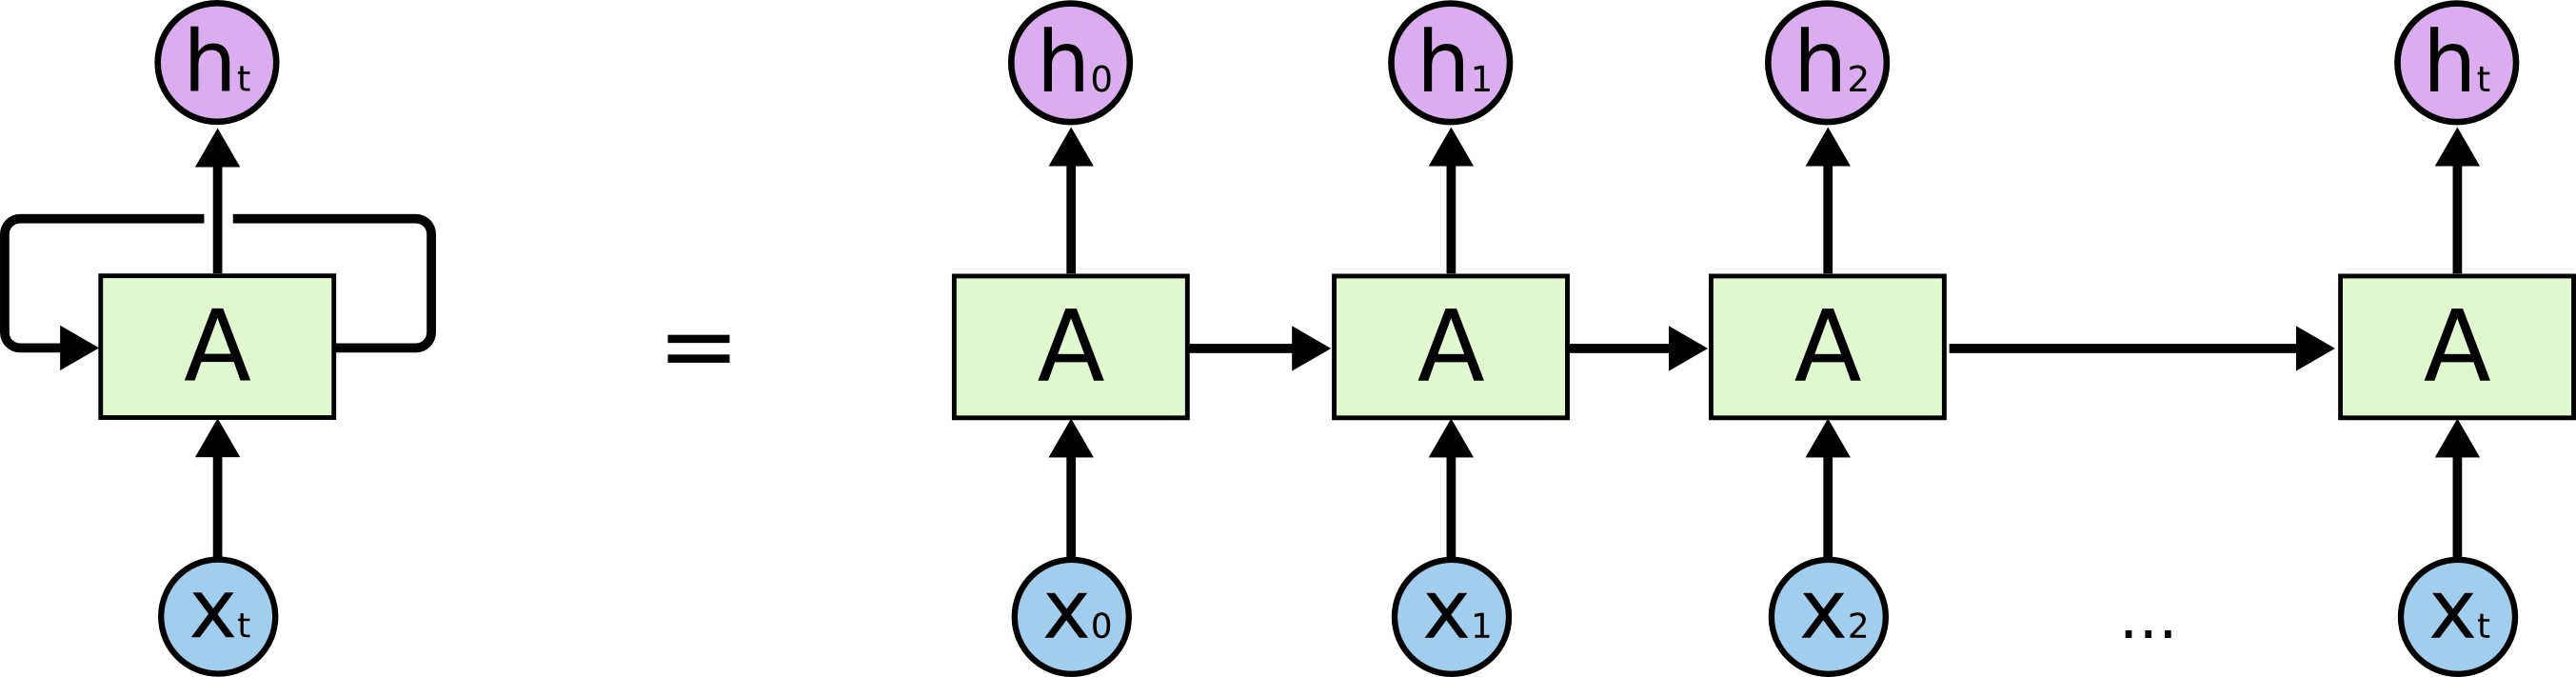
\includegraphics [scale=0.4]{rnn_structure}
	\caption{The structure of Recurrent neural network} 
	\label{img:rnn_structure}  
\end{figure}

However, this type of NN has problems called "Vanishing Gradient and Gradient Explosion Problems". 
This problem was studied in detail in \cite{rnn_problems}. Therefore, the most successful for 
practical issues are modified RNN. I will use the most popular type - Long Short Term Memory networks.

LSTMs are explicitly designed to avoid the long-term dependency problem. Remembering information for long periods of time is practically their default behavior. This features is achieved by more complex structure.
We can compare both architectures in Figure \ref{img:SimpleRNN}\cite{colah_lstm} and Figure \ref{img:LSTM}\cite{colah_lstm}.

\begin{figure}[ht] 
	\center
	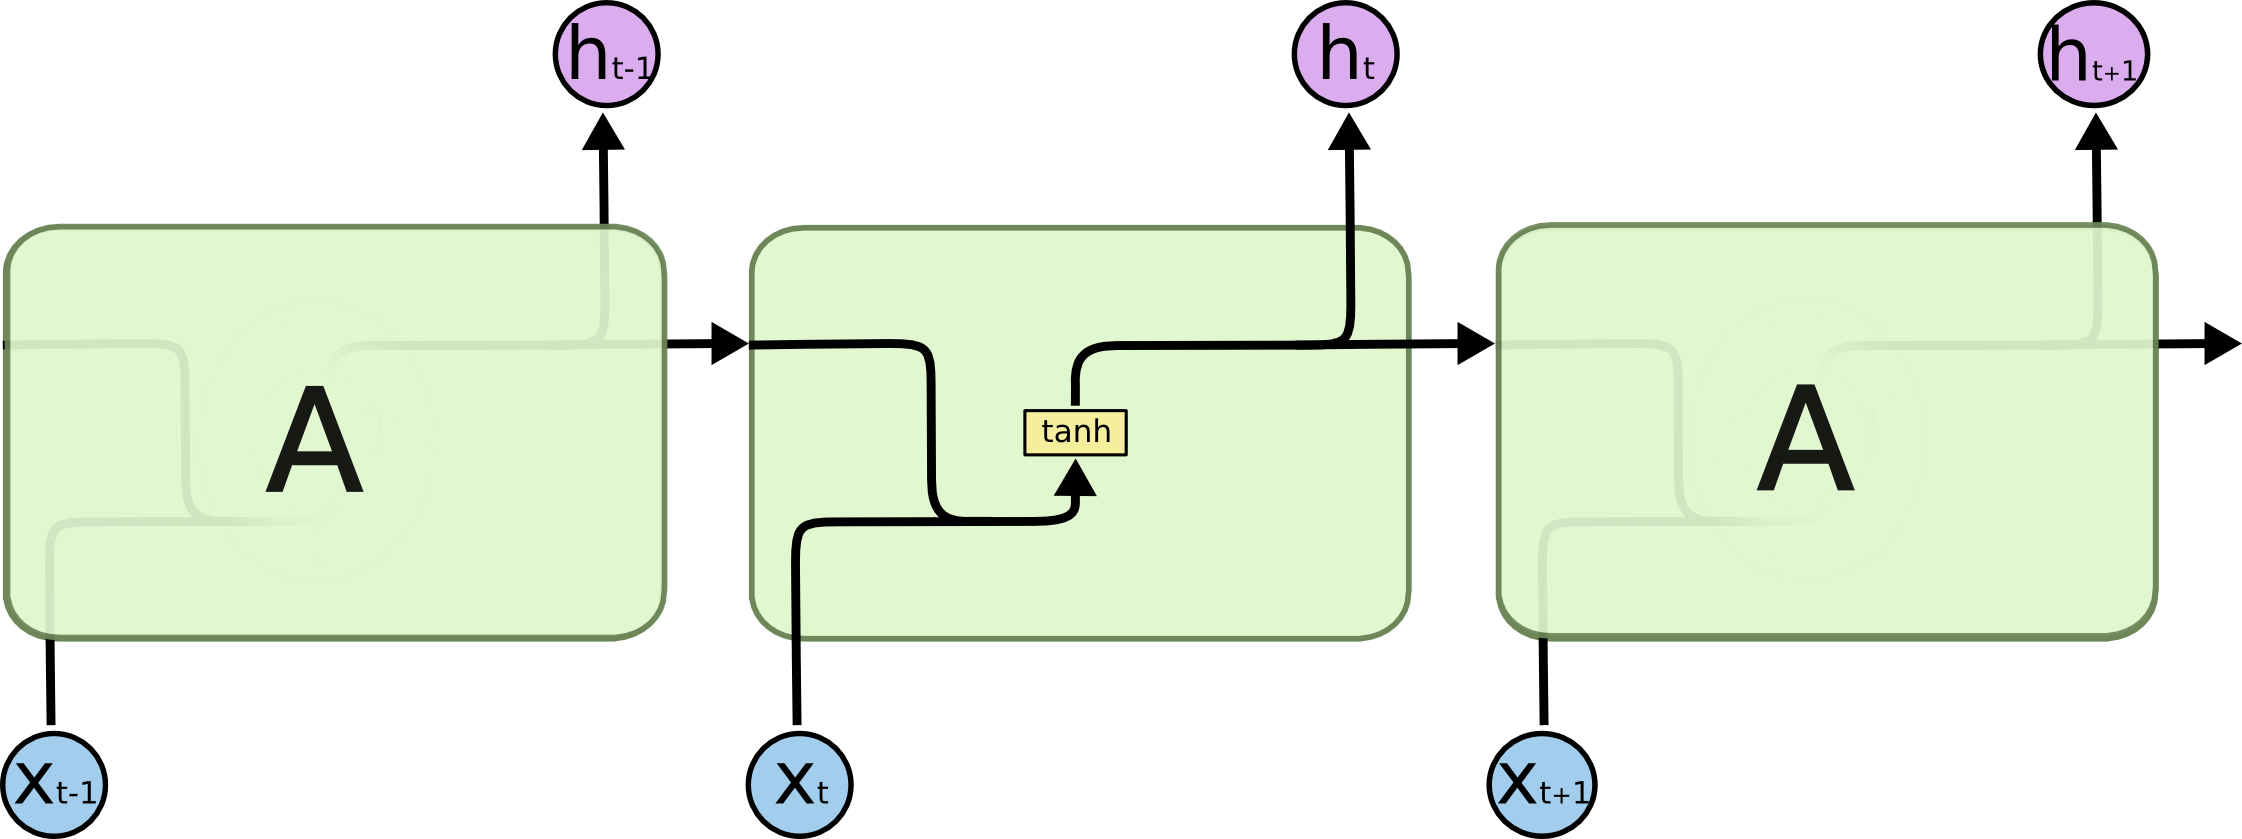
\includegraphics [scale=0.4]{SimpleRNN}
	\caption{The architecture of Recurrent neural network} 
	\label{img:SimpleRNN}  
\end{figure} 

\begin{figure}[ht] 
	\center
	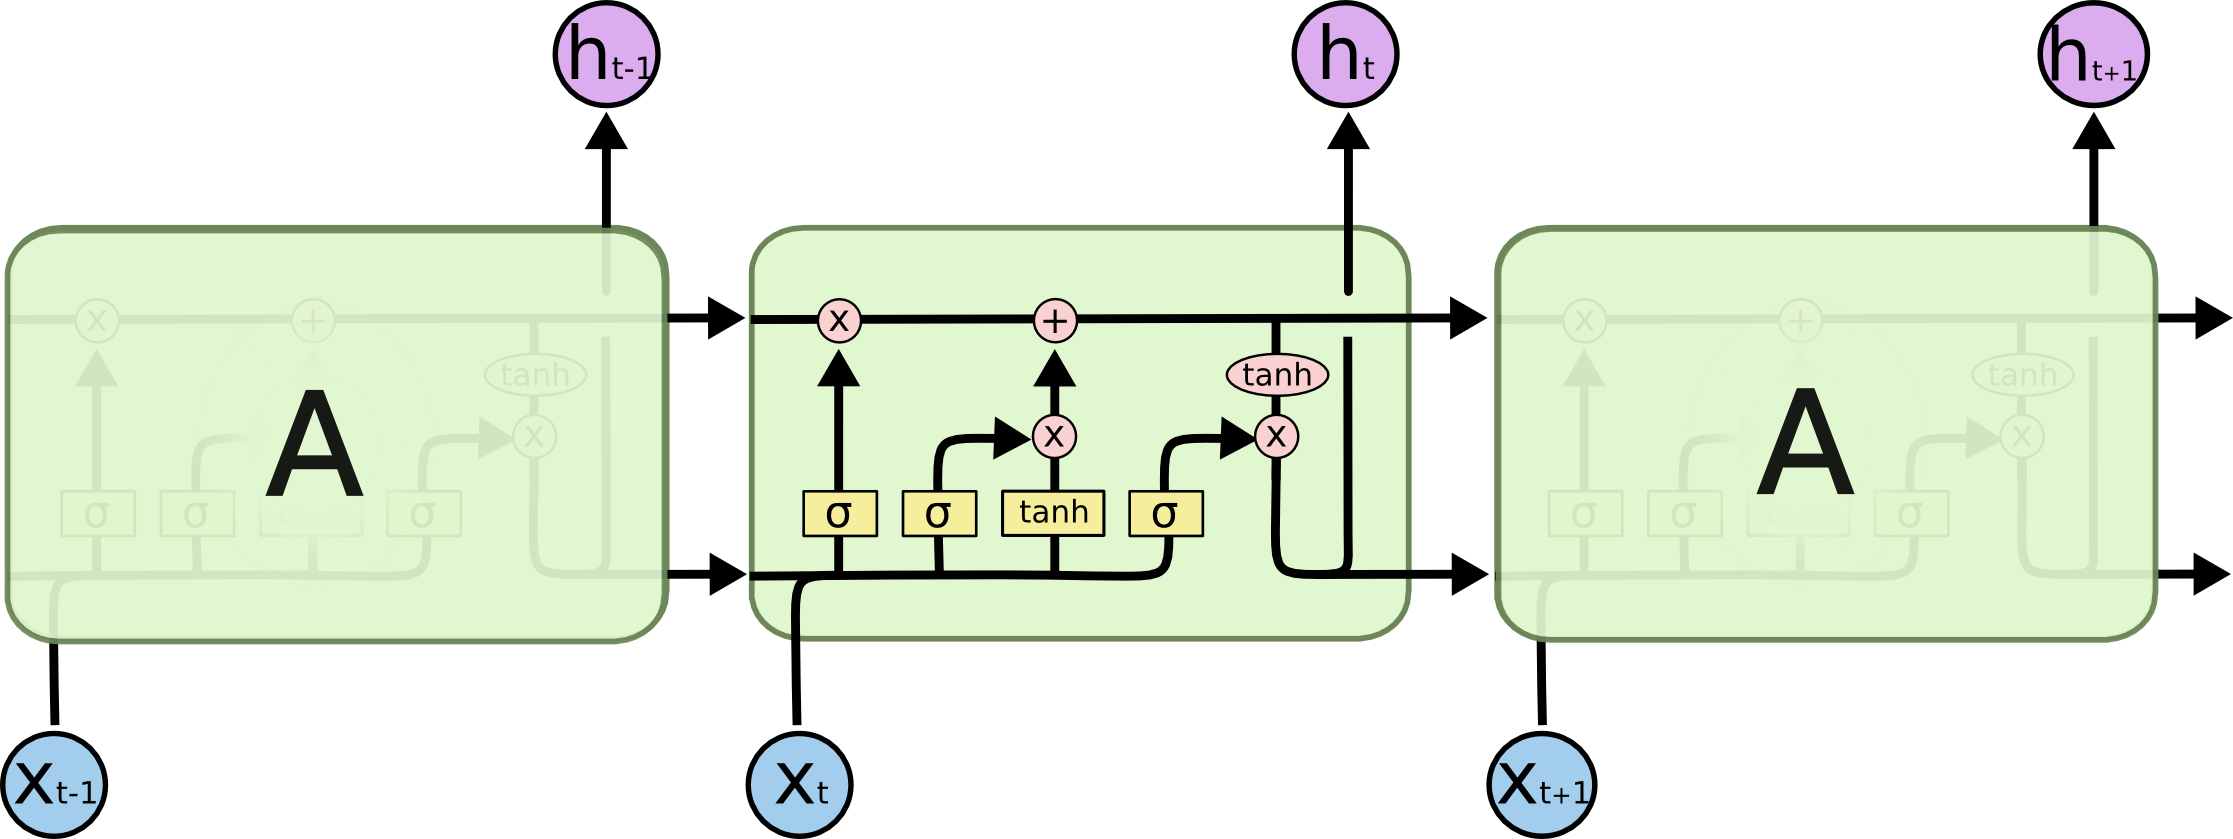
\includegraphics [scale=0.4]{LSTM}
	\caption{The architecture of Long Short Term Memory neural network} 
	\label{img:LSTM}  
\end{figure} 

The first step in LSTM is to decide what information we are going to throw away from the cell state. This decision is 
made by a sigmoid layer called the forget gate layer which 
looks at $h_{t-1}$ and $x_t$, and outputs a number between 0 
and 1 for each number in the cell state $C_{t-1}$.

\begin{equation}
f_t = \sigma(W_f[h_{t-1}, x_t] + b_f)
\end{equation}

The next step is to decide what new information we’re going to store in the cell state. This has two parts. First, a sigmoid layer called the input gate layer decides which values we’ll update. Next, a $tanh$ layer creates a vector of new candidate values, $\tilde{C}_t$, that could be added to the state. In the next step, we combine these two to create an update to the state.

\begin{equation}
i_t = \sigma(W_i[h_{t-1}, x_t] + b_i)
\end{equation}

\begin{equation}
\tilde{C}_t = \tanh(W_C[h_{t-1}, x_t] + b_C)
\end{equation}

To update the old cell state, $C_{t-1}$, into the new cell state $C_t$ we multiply the old state by $f_t$, forgetting the things we decided to forget earlier. Then we add $i_t*\tilde{C}_t$. This is new candidate values, scaled by how much we decided to update each state value.

\begin{equation}
\tilde{C}_t = f_t*{C}_{t-1} + i_t*\tilde{C}_t
\end{equation}

Finally, it is necessary to decide what will go to output. This output will be based on our cell state, but will be a filtered version. First, we run a sigmoid layer which decides what parts of the cell state we’re going to output. Then, we put the cell state through $\tanh$ (to push the values to be between -1 and 1) and multiply it by the output of the sigmoid gate, so that we only output the parts we decided to \cite{colah_lstm} .

\begin{equation}
o_t = \sigma(W_o[h_{t-1}, x_t] + b_o)
\end{equation}

\begin{equation}
h_t = o_t * \tanh(C_t)
\end{equation}

\subsection{Advantages and drawbacks of different architectures} 

Recurrent Neural Networks have intuitive sense in NLP tasks. They reflect the way we process the language : reading sequentially from left to right. 
In contrary, CNNs which widely are used in Computer Vision have such features as Location Invariance and local Compositionality made intuitive sense for images, but not so much for NLP because it is important where a word appears in the sentence. Pixels close to each other are likely to be semantically related , but the same isn’t always true for words.  In many languages, parts of phrases could be separated by several other words. The compositional aspect isn’t obvious either. Clearly, words are compose in some ways, like an adjective modifying a noun, but how exactly this works, what higher level representations actually “mean” isn’t as obvious as in the Computer Vision case. Fortunately, this doesn’t mean that CNNs don’t work.  All models are wrong, but some are useful. It turns out that CNNs applied to NLP problems perform quite well. The simple Bag of Words model is an obvious oversimplification with incorrect assumptions, but has nonetheless been the standard approach for years and lead to pretty good results.

A big argument for CNNs is that they are very fast. Very fast. Convolutions are a central part of computer graphics and are implemented on a hardware level on GPUs. Compared to something like n-grams, CNNs are also efficient in terms of representation. With a large vocabulary, computing anything more than 3-grams can quickly become expensive. Even Google does not provide anything beyond 5-grams. Convolutional Filters learn good representations automatically, without representing the whole vocabulary. It’s completely reasonable to have filters of the size larger than 5.\cite{wildml}
In the next chapter, I will implement both architectures and evaluate them.

\subsection{Summary of the section}

The second section provides a theoretical overview of different methods for textual information 
encoding such as Bag-of-words and embeddings. 
We also deeply analyzed different architectures of neural networks which 
are useful for text classification problem.            % Глава 2
\chapter{\uppercase{Testing and practical application of text classification using software}} \label{chapt3}
\section{Software selection} \label{sect3_1}

The most popular languages in data analysis area are Python and R.
Python3 language was chosen as more convenient for machine learning and beyond variety of libraries, including:

\begin{itemize}
	\item pandas
	\item sklearn
	\item gensim
	\item keras
	\item tensorflow
	\item matplotlib
	\item psycopg2
\end{itemize}

The prototyping of models was made in separate Jupyter notebooks and then re-factored into 
project using the Python IDE for developers be JetBrains company - PyCharm. 
The server with  Intel(R) Core(TM) i7-4770 CPU @ 3.40GHz, 15 $\times$ 2 GB DDR3-1333 was used. 

As a word vectors representation I used pre-trained word vectors which were trained on Wikipedia using fastText technique by Facebook research team and shared to the community \cite{fasttext}. These vectors in dimension 300 were obtained using the skip-gram model with default parameters.

To build deep neural network models my main requirements for the framework were:
\begin{itemize}
	\item well described documentation
	\item simplicity of usage
	\item learning speed
	\item reliability
\end{itemize}

Among a wide range of frameworks available in open source: 
CNTK, Theano, MAXNET, Lasagne - Tensorflow framework was chosen. 
Tensorflow has a flexible architecture allows easy deployment of computation across a variety of platforms (CPUs, GPUs, TPUs). To speed up the experiments with architecture of NN, I switched to a high-level neural networks API, written in Python and capable of running on top of TensorFlow. 

\section{Dataset selection and exploration} \label{sect3_2}

The target attribute to be predicted is the category of the advertisements. The category is represented by the two-level hierarchy. The parent category consists of 16 categories which then branches into 183 subcategories. These categories can be mapped together in the following way:

\begin{table}[h]
	\centering
	\caption{The hierarchy of categories}
	\label{my-label}
	\begin{tabular}{|c|c|}
		\hline
		
		lvl2     & category ID     \\
		\hline
		lvl1 		  & identifier of the parent category		 \\
		\hline
		name	 		  & category name		 \\
		\hline
	\end{tabular}
\end{table}

The dataset contains 455,000 ads classified into 183 categories. 
The sample of dataset can be seen from Table \ref{data_structure}.
First, let us get familiar with data and how it distributes between categories.
As it can be clearly seen from Table \ref{general} we have 2 categorical 
and 2 numerical variables and our data does not have any missing fields. 
It is good to start examining our data by each variable separately. 
From Table \ref{lvl1} we can see that data is not distributed equally between 
categories. First-level categories with number 6,5,1 consist almost of half 
of all advertisements. That means that our data is imbalanced and we can not 
use accuracy as only one metric for evaluation. 
Then if we take a look at second-level categories Table \ref{lvl2} we will see even the worst picture: one third of the date is concentrated in the categories which are marked 29,14 and 55 respectively. 
That means that it is necessary to use techniques to regularize distributions: under/over sampling or weight balanced.

For evaluation such metrics as categorical\_accuracy
, categorical\_crossentropy, loss, timing and top\_k\_categorical\_accuracy were chosen. 


\begin{table}[]
	\centering
	\caption{Structure of the data files}
	\label{data_structure}
	\begin{tabular}{| p{1cm} | p{1cm} | p{3cm} | p{7cm} |}
		\hline
		\textbf{lvl1} & \textbf{lvl2} & \textbf{titles}                  & \textbf{descriptions}                                                                       \\ \hline
		6             & 29            & Clean Toyota Camry 2008 Silver   & Fairly used Toyota 08 Camry with no problems V4 engine fabric seats and interior            \\ \hline
		5             & 25            & Look Unique                      & Nice, quality, adorable,unique dress available now, whatsapp me                             \\ \hline
		6             & 29            & Mercedes Benz Ml 430 2001 Silver & mercedes benz ml430 , 2001 model in good condition , engine and gear box ok, ac , cd player \\ \hline
		5             & 25            & Versace Shirt Dress              & Adorable versace shirt dress, whatsapp me on \_large\_number\_                              \\ \hline
		5             & 25            & Addidas Jumpsuit                 & Nice quality addidas jumpsuit available, whatsapp me                                        \\ \hline
	\end{tabular}
\end{table}


\begin{table}[h]
	\centering
	\caption{Training set general information}
	\label{general}
	\begin{tabular}{|c|c|}
		\hline
	\textbf{	Number of variables     }      & 4      \\
		\hline
	\textbf{	Numeric variables}	 		  & 2		 \\
		\hline
	\textbf{	Categorical	variables} 		  & 2		 \\
		\hline
		\textbf{Number of observations }       & 455000  \\
		\hline
		\textbf{Total Missing (\%) }           & 0.0\%    \\
		\hline
		\textbf{Total size in memory }         & 57.7 MiB \\
		\hline
		\textbf{Average record size in memory} & 48.0 B  \\
		\hline
	\end{tabular}
\end{table}


\begin{table}[h]
	\centering
	\caption{Information about first-level categories}
	\label{lvl1}
	\begin{tabular}{|l|l|l|l|}
		\hline
	\textbf{Value }             & \textbf{Count}  & \textbf{Frequency} (\%) \\ \hline
		6                & 207695 & 20.8\%           \\ \hline
		5                & 184934 & 18.5\%           \\ \hline
		1                & 133135 & 13.3\%           \\ \hline
		4                & 97799  & 9.8\%            \\ \hline
		3                & 87574  & 8.8\%           \\ \hline
		110              & 60214  & 6.0\%            \\ \hline
		9                & 55459  & 5.5\%            \\ \hline
		27               & 52419  & 5.2\%            \\ \hline
		47               & 38985  & 3.9\%            \\ \hline
		140              & 36442  & 3.6\%           \\ \hline
		Other values (6) & 45344  & 4.5\%            \\ \hline
	\end{tabular}
\end{table}


\begin{table}[H]
	\centering
	\caption{Information about second-level categories}
	\label{my-label}
	\begin{tabular}{|l|l|l|}
		\hline
		\textbf{Value }             & \textbf{Count}  & \textbf{Frequency} (\%) \\ \hline
		29                 & 194714 & 19.5\%         \\ \hline
		14                 & 115471 & 11.5\%         \\ \hline
		55                 & 72050  & 7.2\%          \\ \hline
		25                 & 61308  & 6.1\%          \\ \hline
		16                 & 32719  & 3.3\%          \\ \hline
		20                 & 23298  & 2.3\%          \\ \hline
		169                & 18743  & 1.9\%          \\ \hline
		42                 & 18490  & 1.8\%          \\ \hline
		44                 & 17740  & 1.8\%          \\ \hline
		279                & 15544  & 1.6\%          \\ \hline
		Other values (172) & 429923 & 43.0\%         \\ \hline
	\end{tabular}
\end{table}


\begin{table}[H]
	\centering
	\caption{Information about categorical features}
	\label{my-label}
	\begin{tabular}{llll}
		\hline
\multicolumn{1}{|l|}{\textbf{Column}} & \multicolumn{1}{l|}{\textbf{Distinct count}} & \multicolumn{1}{l|}{\textbf{Unique (\%)}} & \multicolumn{1}{l|}{\textbf{Missing (\%)}} \\ \hline
		\multicolumn{1}{|l|}{titles}       & \multicolumn{1}{l|}{619948}         & \multicolumn{1}{l|}{62.0\%}      & \multicolumn{1}{l|}{0.00\%}       \\ \hline
		\multicolumn{1}{|l|}{descriptions} & \multicolumn{1}{l|}{869554}         & \multicolumn{1}{l|}{87.0\%}      & \multicolumn{1}{l|}{0.00\%}       \\ \hline
	\end{tabular}
\end{table}


I decided to divide the whole dataset into train.csv / test.csv files which have the following structure:training set contains 400000 observation and control sample - 55,000 ads. 

\clearpage
\section{Data preparation} \label{sect3_3}
The following diagram describes steps which were taken to process texts Figure ~\ref{img:p3_preprocessing}.

\begin{figure}[H] 
	\center
	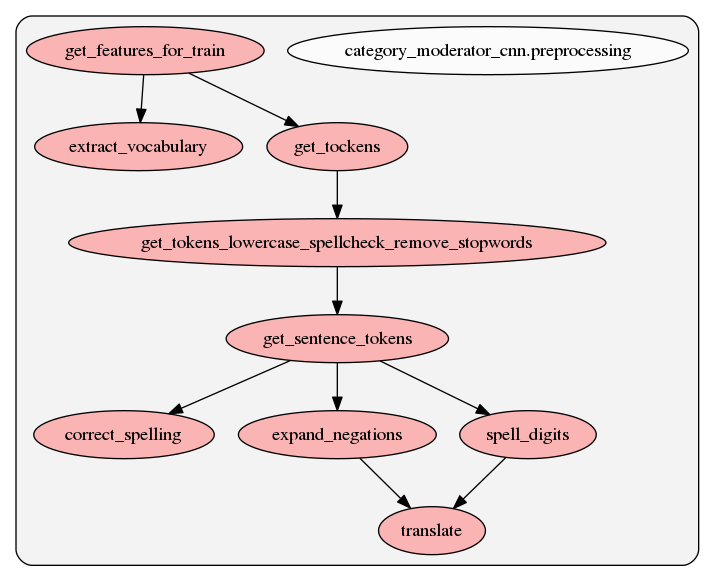
\includegraphics [scale=0.5] {p3_preprocessing.png} 
	\caption{Simplified event structure of data preprocessing}
	\label{img:p3_preprocessing}  
\end{figure}


\noindent 1.Tokenize Text

The given text was split by spaces and then lemmatized.

\noindent 2. Remove infrequent words

Words appearing less than 3 times in the whole corpus were removed. It’s a good idea to remove these infrequent words because a huge vocabulary will make our model slow to train and not all these words are presented in pretrained embeddings. 
Special attention should be paid to numbers which can be represented as price, year, mobile number. The telephone numbers occur really frequently in advertisements, but in most cases, they are unique because different people have their telephone numbers - the information about whether a telephone number presented in the text or not is meaningful. I used regular expressions to replace all numbers with the words \_large\_number\_, \_small\_num\_,  \_price\_, \_year\_. which gave me a possibility not to lose precious information. 
\\

\noindent
\textit{\textbf{r'[0-9a-z\_]+@[a-z]+\.[a-z]+': '\_email\_', \\
r'[0-9]{5,20}': '\_large\_number\_',\\
r'[1-9][0-9]*k': '\_price\_',
\\
r'[1-9][0-9]+?,[0-9]*': '\_price\_',
\\
r'[1-9][0-9]*?,[0-9]* thousand': '\_price\_',
\\
r'19[0-9]{2}': '\_year\_',
\\
r'200[0-9]': '\_year\_',
\\
r'201[0-8]': '\_year\_',
\\
r'[0-9]+': '\_small\_num\_',}}
\\

\noindent 3. Correct misspellings

I analyzed properly the most frequent cases where users make mistakes. Then I created a dictionary which consists of wrong and right written words, so each time when the wrong written word appears, it is replaced with the right written equivalent. 

\newcolumntype{b}{X}
\newcolumntype{s}{>{\hsize=.5\hsize}X}

\begin{table}[h]
	\centering
	\caption{Simplified event structure of data preprocessing}
	\label{my-label}
	\begin{tabular}{| p{7cm} | p{10cm} |}
%	\begin{tabulary}{1.0\textwidth}{|L|L|L|L|L|L}
		\hline
		\textbf{Functions}                                    & \textbf{Explanation}                                                                                                                \\ \hline
		get\_features\_for\_train                             & function which unify uploads of raw data and calls nested functions                                                                   \\ \hline
		extract\_vocabulary                                   & form vocabulary from unique words                                                                                                   \\ \hline
		get\_tokens                                           & parallel batch execution of texts preprocessing 
		\\ \hline
		get\_tokens\_lowercase\_spellcheck\ & wrap over get\_sentence\_tokens which set necessary flags for it                                                                    \\ \hline
		get\_sentence\_tokens                                 & receive single sentence, break it into tokens, make all of them to lowercase, correct spelling mistakes and replace specific words \\ \hline
		correct\_spelling                                     & correct spelling mistakes using dictionary with around 15000 most common mistakes                                                   \\ \hline
		expand\_negations                                     & replace mobile phones, dates, prices, and common abbreviation with specific words such as \_year\_, price,  \_large\_number\_ etc.  \\ \hline
		spell\_digits                                         & single digits are replaced with corresponding word 1 $\rightarrow$ one …                                                                          \\ \hline
		translate                                             & function which makes replacement of words                                                                                           \\ \hline
	\end{tabular}
\end{table}



\noindent 4. Build embeddings 
The following diagram describes steps which where made to build embeddings for each word Figure \ref{img:p3_sequences_fasttext}.

\begin{figure}[ht] 
	\center
	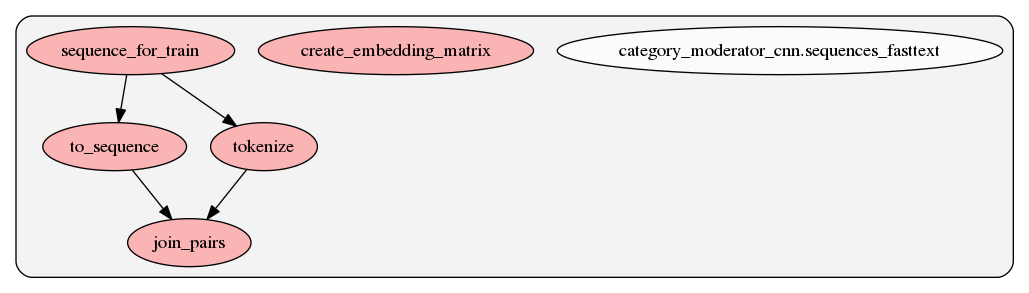
\includegraphics [scale=0.45] {p3_sequences_fasttext.png}
	\caption{Build embeddings structure} 
	\label{img:p3_sequences_fasttext}  
\end{figure}


The input to Neural Networks are vectors, not strings. The mapping between words and indices was created, index\_to\_word, and word\_to\_index. For example,  the word “buy” may be at index 201. 



\begin{table}[h]
	\centering
	\caption{Simplified event structure of data preprocessing}
	\label{my-label}
	\begin{tabular}{| p{7cm} | p{10cm} |}
		%	\begin{tabulary}{1.0\textwidth}{|L|L|L|L|L|L}
		\hline
		\textbf{Functions}                                    & \textbf{Explanation}                                                                                                                \\ \hline
		sequence\_for\_train                             & load preprocessed tokens from the previous model and use functions listed below to create sequences of indices which corresponds to particular word.                                                                    
		\\ \hline
		to\_sequence                                   & encode each word with the corresponding index        and organize them into sequences of indices with the particular length                                                      \\ \hline
		tokenize                                           & build and save tokenizer which maps words and their indices 
		\\ \hline
		join\_pairs &  helpful function for transformation                                                      
		\\ \hline
		create\_embedding\_matrix                                 & build the embedding matrix for unique words from our dataset. It will have the structure word represented by its index in our vocabulary and the corresponding vector from the pre-trained embedding model. \\ \hline

	\end{tabular}
\end{table}





\clearpage
\section{Network design and training} \label{sect3_4}
The following diagram shows structure of the final module, which main responsibility is to train model. \ref{img:p3_train}.

\begin{figure}[H] 
	\center
	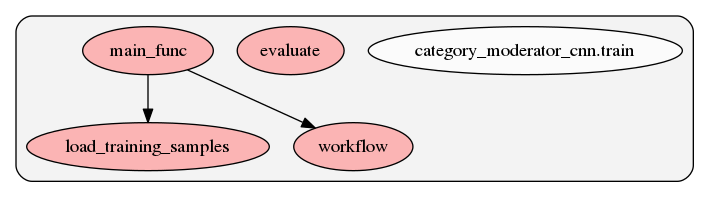
\includegraphics [scale=0.5] {p3_train.png}
	\caption{Train model structure} 
	\label{img:p3_train}  
\end{figure}


In this module I implemented different types of neural networks. Each network design module describes only
one type of networks, which makes text classification. After the design of NN was implemented it should be trained. Apart from the training part this module saves training statistics \ref{img:p3_custom_callbacks} such as: 
\begin{itemize}
	\item categorical accuracy
	\item top k categorical accuracy
	\item batch timer
	\item categorical loss
	\item histograms of NN weights
\end{itemize}

These metrics will be used to judge the performance of our model. 
Such statistics give more information about changes in the neural network on each step of training. 
As tested network types on this step, I choose bidirectional recurrent network 
and convolutional network with different window sizes. 


\begin{figure}[H] 
	\center
	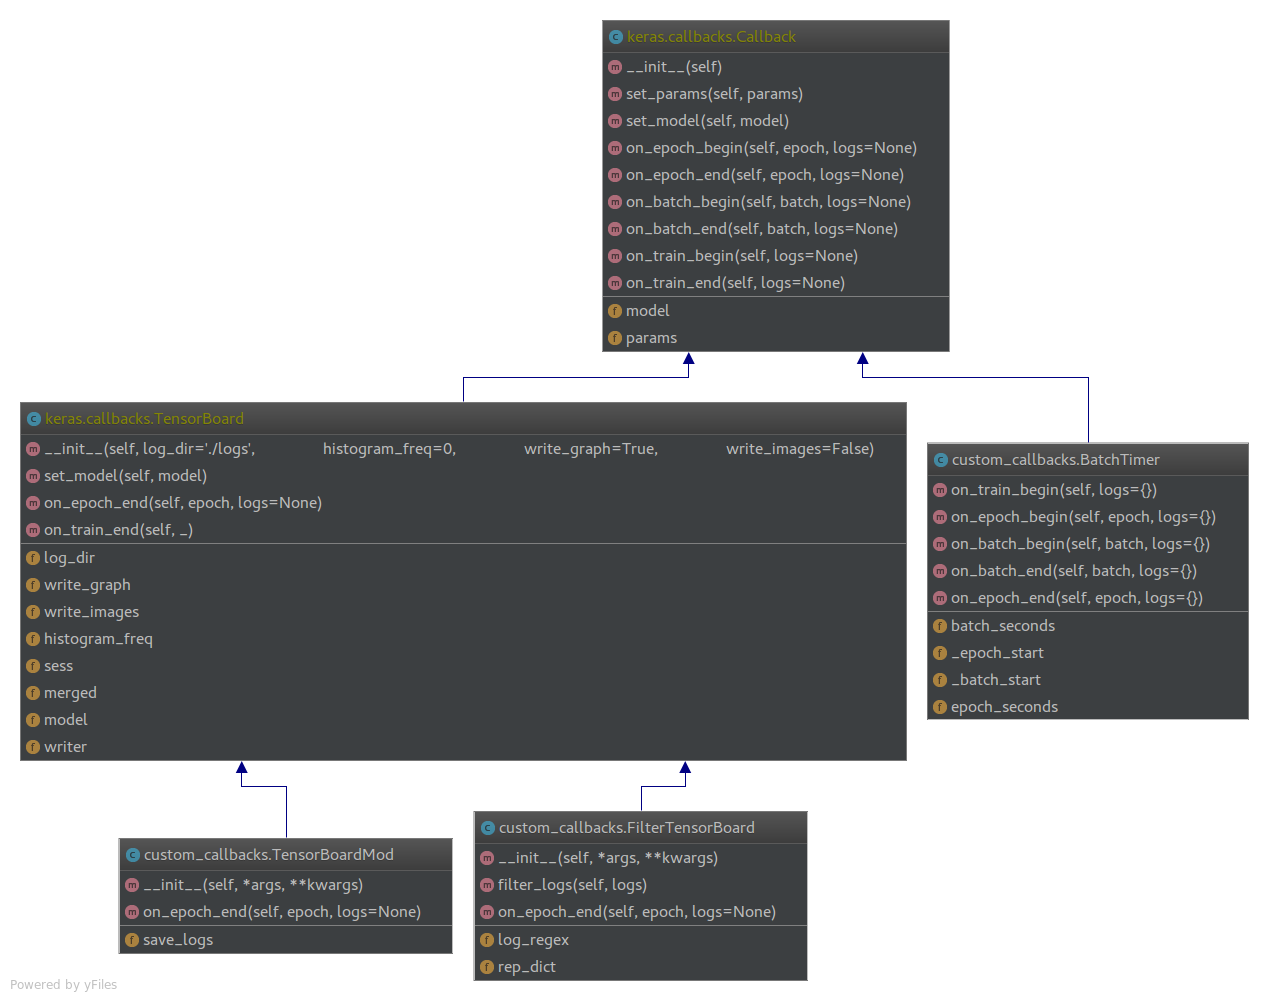
\includegraphics [scale=0.25] {p3_custom_callbacks.png} 
	\caption{Metrics which were logged} 
	\label{img:p3_custom_callbacks} 
\end{figure}

\section{Summary of the section}\label{sect3_5}
This section argues the usage of the selected software. A detailed analysis of the data was provided. 
Also, we went through the implementation process: from the raw data to the trained model.
An explanation of the most significant functions was made. 
           % Глава 3
\chapter{\uppercase{Classification results evaluation}} \label{chapt4}

\section{General steps} \label{sect4_1}
\noindent
In this section I need to:
\begin{itemize}
	\item visualize results of each training step, to understand hyperparameters better
	\item estimate networks by types 
	\item choose hyperparameters to gain the best evaluation metrics  
	\item train each network on different amount of epochs
	\item save network parameters and weights after each epoch. It will give me a possibility to restore the best model if network accuracy goes down.
\end{itemize}

\noindent
Training time is a very important parameter. Therefore, I would like to train NN models which have nearly the same training time. To make it easier to understand the results of NN, a famous suite of visualization tools called TensorBoard was used. With TensorBoard it is possible to visualize graphs, plot quantitative metrics and show additional data like images passing through it.  


\section{Base line model} \label{sect4_2}

Firstly, I built the baseline model which CNN models should achieve in the future. I started this step with LSTM networks, as most often mentioned in the articles on NLP problems. At this step I was trying different configurations of LSTM parameters. The architecture which gave me the best score is shown in Figure \ref{img:part4-bilstm}. According to my experiments bidirectional recurrent networks perform better than the same type and same size by parameters one directional networks, therefore it was chosen as the main layer. As input to the NN I gave two embedded sequences of words: one for the description of advert, the other for title. This model has the bi-LSTM layer with 100 units. Each sequence goes through the bi-LSTM layer and then merged together. To solve overfitting in this model I used BatchNormalization and dropout. LSTM dropout rate was chosen manually and was equal to 0.332. Besides the bi-LSTM layer, there are two fully connected layers: one at the end because we want to estimate probabilities for each class, so it has 183 neurons in it and one in the middle with 130 neurons. As a training algorithm I chose Adam with default parameters: (lr=0.001, beta\_1=0.9, beta\_2=0.999, epsilon=1e-08, decay=0.0). As I have mentioned earlier, to better understand the network I visualize the histograms and percentile weights in each layer. The model was trained on 15 epochs.


\begin{figure}[ht] 
	\center
	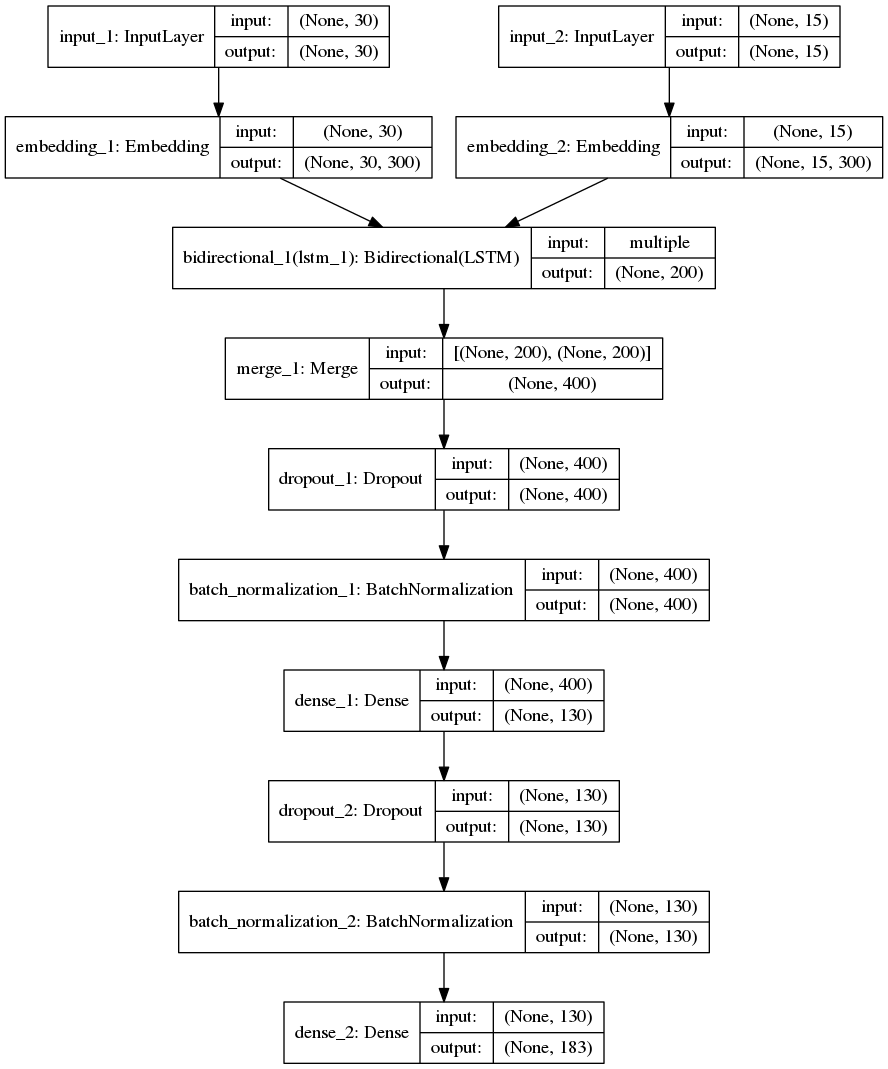
\includegraphics [scale=0.4] {part4/bilstm_architecture.png} 
	\caption{Architectures of Bi-LSTM models with 100 units } 
	\label{img:part4-bilstm} 
\end{figure}

As can be seen from the results of model training in Figure \ref{img:/bilstm_val_category_accuracy}, categorical accuracy on the training set and validation set performs equally well: 0.7975 and 0.8203 respectively. Surprisingly, the results on train are slightly better than on training data.   

\begin{figure}[ht]
	\begin{minipage}[ht]{1\linewidth}
		\center{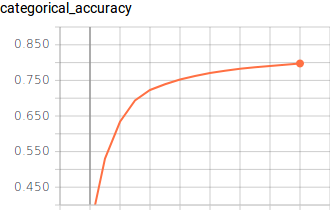
\includegraphics[width=0.5\linewidth]{part4/bilstm_train_category_accuracy}}
	\end{minipage}
	\hfill
	\begin{minipage}[ht]{1\linewidth}
		\center{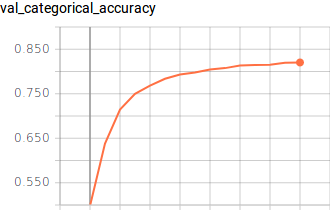
\includegraphics[width=0.5\linewidth]{part4/bilstm_val_category_accuracy}}
	\end{minipage}
	\caption{Models train and validation categorical accuracy by epochs}
	\label{img:/bilstm_val_category_accuracy}  
\end{figure}

Figure \ref{img:bilstm_val_category_crossentropy} shows that categorical cross entropy decrease on each epoch as it was expected. After 15 epochs results were the following: 0.8532 on the training set and 0.7478 on test.    

\begin{figure}[ht]
	\begin{minipage}[ht]{1\linewidth}
		\center{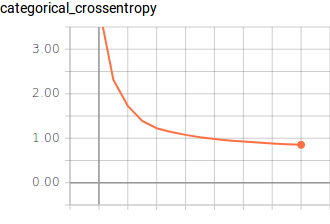
\includegraphics[width=0.5\linewidth]{part4/bilstm_train_category_crossentropy}}
	\end{minipage}
	\hfill
	\begin{minipage}[ht]{1\linewidth}
		\center{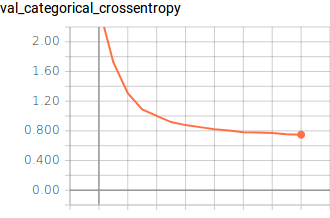
\includegraphics[width=0.5\linewidth]{part4/bilstm_val_category_crossentropy}}
	\end{minipage}
	\caption{Models train and validation category crossentropy by epochs}
	\label{img:bilstm_val_category_crossentropy}  
\end{figure}

The most important metric for this task was top categorical accuracy which can be seen in Figure \ref{img:bilstm_val_top_k_accuracy}. On training data the model showed 0.9189 accuracy and on the test data - 0.9319.   

\begin{figure}[ht]
	\begin{minipage}[ht]{1\linewidth}
		\center{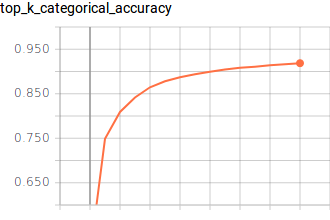
\includegraphics[width=0.5\linewidth]{part4/bilstm_train_top_k_accuracy}}
	\end{minipage}
	\hfill
	\begin{minipage}[ht]{1\linewidth}
		\center{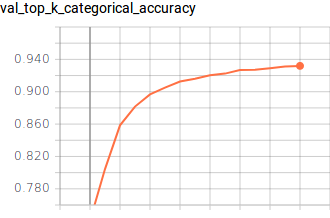
\includegraphics[width=0.5\linewidth]{part4/bilstm_val_top_k_accuracy}}
	\end{minipage}
	\caption{Models train and validation top k accuracy by epochs}
	\label{img:bilstm_val_top_k_accuracy}  
\end{figure}

Additional metrics which interested me in these experiments was time per epoch. These results can be seen in Figure \ref{img:bilstm_timing}.

\clearpage
\begin{figure}[ht] 
	\center
	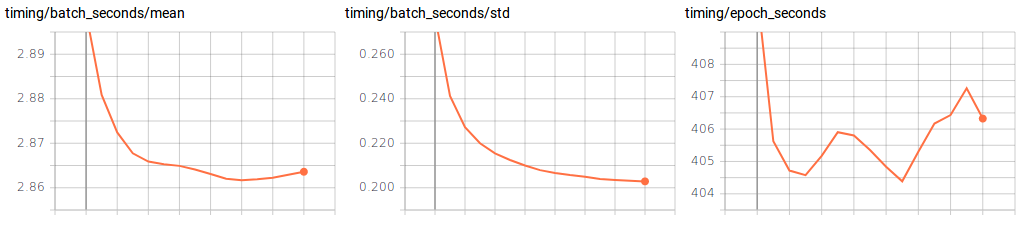
\includegraphics [scale=0.5] {part4/bilstm_timing}
	\caption{Models batch time by epochs} 
	\label{img:bilstm_timing}  
\end{figure}


Histograms give much information about what is happening with the network. I decided to pay attention to histograms which were output from the recurrent network - that show bi-LSTM behavior and weights for first layer of feedforward network. I did not find a descriptive explanation for how to interpret these kinds of graphics, so I followed basic knowledge from statistics. 

\begin{figure}[ht]
	\begin{minipage}[ht]{1\linewidth}
		\center{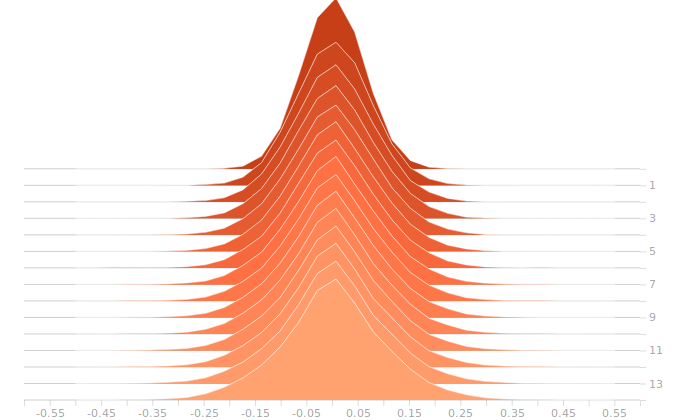
\includegraphics[width=0.5\linewidth]{part4/bilstm_forward_lstm_1_recurrent_kernel_0} \\ а}
	\end{minipage}
	\hfill
	\begin{minipage}[ht]{1\linewidth}
		\center{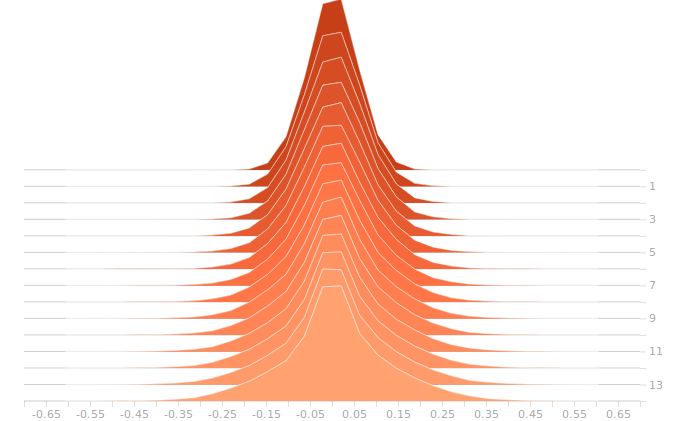
\includegraphics[width=0.5\linewidth]{part4/bilstm_backward_lstm_1_recurrent_kernel_0} \\ b}
	\end{minipage}
	\caption{Bi-LSTM 100 units. Histogram of output from forward recurrent layers (a); histogram of weights from backward recurrent layers (b)}
	\label{img:Bi-LSTM 100 units. Histogram of output from forward recurrent}  
\end{figure}


According to Figures \ref{img:/bilstm_val_category_accuracy}, \ref{img:bilstm_val_category_crossentropy}, \ref{img:bilstm_val_top_k_accuracy} model was not overfitted. Histograms of outputs from feed forward and backward recurrent layers Figure \ref{img:Bi-LSTM 100 units. Histogram of output from forward recurrent} do not change significantly during training process. 
This can be explained by the fact that this layer does not train enough and I think that this network continues to learn thanks to FFNN part Figure \ref{img:bilstm_dense}. I think, that the best shape for the histogram of weights from first FFNN layer will be a normal distribution with higher variance, than after initialization. As we can see the FFNN layer has exactly such behavior which means that it learns some meaningful information. It is possible that more epochs will have a positive effect on the recurrent layer. 

\begin{figure}[ht] 
	\center
	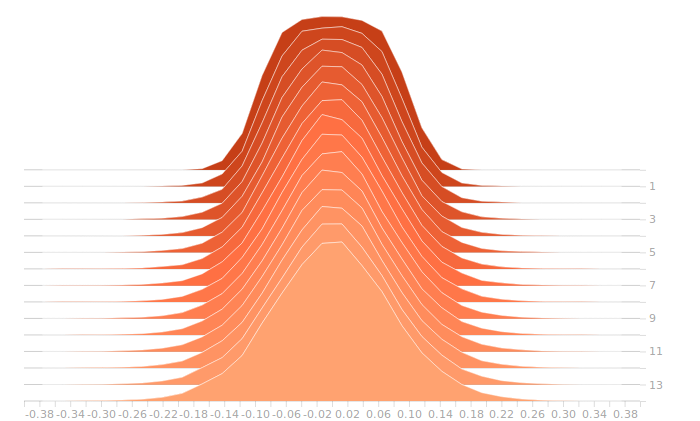
\includegraphics [scale=0.5] {part4/bilstm_dense}
	\caption{Bi-LSTM 100 units. Histogram of weights from first FFNN layer.} 
	\label{img:bilstm_dense}  
\end{figure}

The bi-LSTM model requires a significant amount of computational resources: especially RAM.
Therefore, a batch size was chosen equal to 3048. We can see consumption of resources in Figure \ref{img:resources_BILSTM}


\begin{figure}[ht] 
	\center
	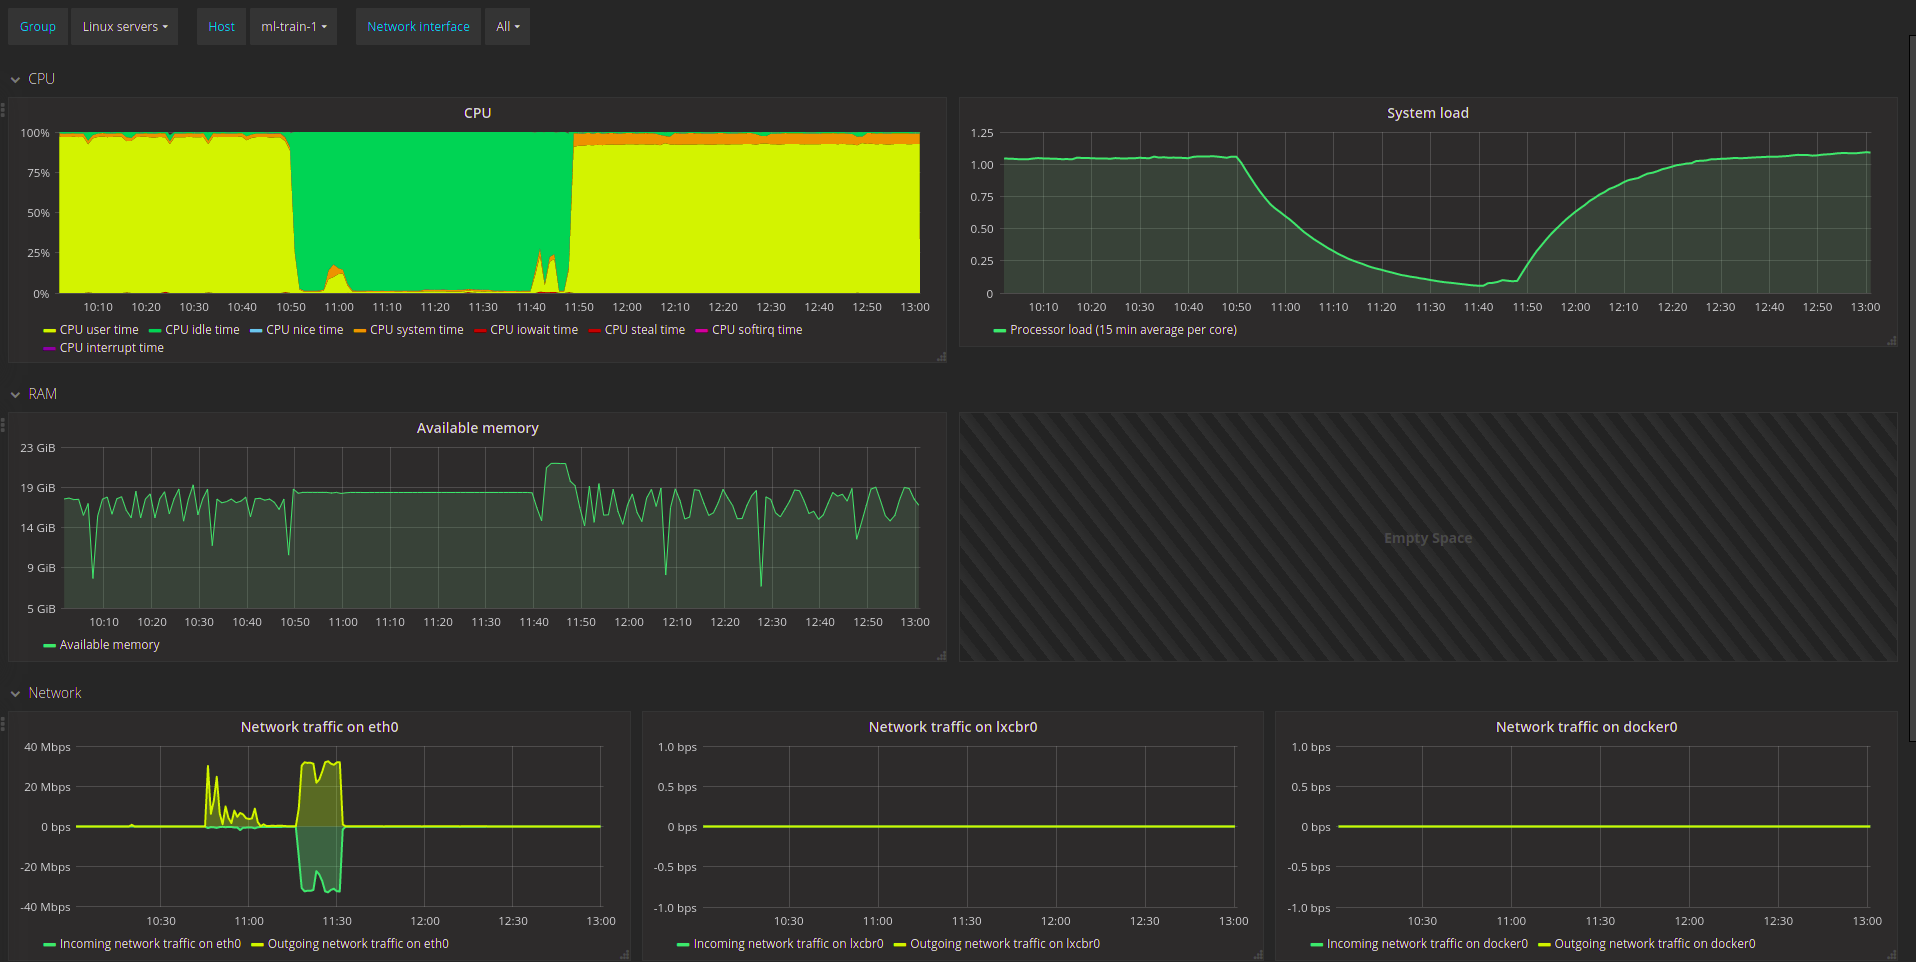
\includegraphics [scale=0.2] {part4/resources_BILSTM}
	\caption{CPU resources which were used while training Bi-LSTM NN.} 
	\label{img:resources_BILSTM}  
\end{figure}


\clearpage
\section{Convolution neural network} \label{sect4_3}

In this part, I would like to show that CNN can perform not worse than recurrent based neural networks. Therefore, I implemented CNN architecture Figure \ref{img:cnn_architecture} which was described in the section \ref{sect2_2_1}. I build three model with different numbers of filters. The smallest one contains 128 filters, middle one - 256 and the biggest - 512. All models were trained with the same number of filter: 3, 4, 5 and dropout rate equals to 0.5. I did not use regularization for convolution layers, but according to my experience, big pooling window also prevent overfitting.Models were trained on 15 epochs.

Let us compare results which different models give. 

\begin{table}[h]
	\centering
	\caption{Analysis of categorical accuracy}
	\label{my-label}
	\begin{tabular}{| p{7cm} | p{3cm} | p{3cm} |}
		%	\begin{tabulary}{1.0\textwidth}{|L|L|L|L|L|L}
		\hline
		\textbf{Number of filters}  & \textbf{Train} & \textbf{Test}                                                    
		\\ \hline
		128   &  0.8165 & 0.8126
		\\ \hline
		256   &  0.8532 & 0.8251 
		\\ \hline
		512   &  0.8885 & 0.8338
		\\ \hline		
	\end{tabular}
\end{table}


\begin{figure}[ht]
	\begin{minipage}[ht]{1\linewidth}
		\center{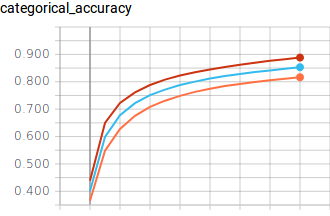
\includegraphics[width=0.5\linewidth]{part4/3CNN_train_category_accuracy}}
	\end{minipage}
	\hfill
	\begin{minipage}[ht]{1\linewidth}
		\center{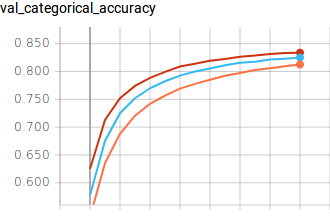
\includegraphics[width=0.5\linewidth]{part4/3CNN_val_category_accuracy}}
	\end{minipage}
	\caption{Models train and validation categorical accuracy by epochs}
	\label{img:3CNN_categorical_accuracy}  
\end{figure}


\begin{table}[h]
	\centering
	\caption{Analysis of category crossentropy}
	\label{my-label}
	\begin{tabular}{| p{7cm} | p{3cm} | p{3cm} |}
		%	\begin{tabulary}{1.0\textwidth}{|L|L|L|L|L|L}
		\hline
		\textbf{Number of filters}  & \textbf{Train} & \textbf{Test}                                                    
		\\ \hline
		128   &  0.8060 & 0.8434
		\\ \hline
		256   &  0.6340 & 0.7746 
		\\ \hline
		512   &  0.4731 & 0.7331
		\\ \hline		
	\end{tabular}
\end{table}

\begin{figure}[ht]
	\begin{minipage}[ht]{1\linewidth}
		\center{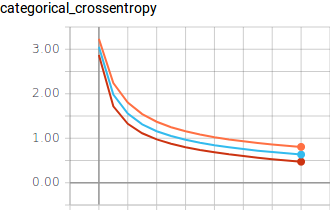
\includegraphics[width=0.5\linewidth]{part4/3CNN_train_category_crossentropy}}
	\end{minipage}
	\hfill
	\begin{minipage}[ht]{1\linewidth}
		\center{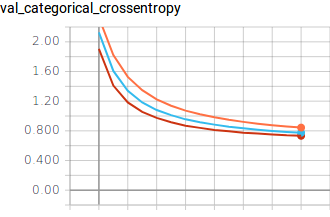
\includegraphics[width=0.5\linewidth]{part4/3CNN_val_category_crossentropy}}
	\end{minipage}
	\caption{Models train and validation category crossentropy by epochs}
	\label{img:3CNN_category_crossentropy}  
\end{figure}


\begin{table}[h]
	\centering
	\caption{Analysis of top k accuracy}
	\label{my-label}
	\begin{tabular}{| p{7cm} | p{3cm} | p{3cm} |}
		%	\begin{tabulary}{1.0\textwidth}{|L|L|L|L|L|L}
		\hline
		\textbf{Number of filters}  & \textbf{Train} & \textbf{Test}                                                    
		\\ \hline
		128   &  0.9259 & 0.9191
		\\ \hline
		256   &  0.9495 & 0.9286 
		\\ \hline
		512   &  0.9696 & 0.9342
		\\ \hline		
	\end{tabular}
\end{table}


According to the results \ref{img:3CNN_categorical_accuracy}, \ref{img:3CNN_category_crossentropy}, \ref{img:3CNN_top_k_accuracy}, \ref{img:3CNN_timing}, I can assume that models having more filters show better accuracy. However, it is noticeable that model with 256 and 512 filters have quite different results on train and test sets (~3-5\% difference). It can be interpreted as overfitting of these models. 


\begin{figure}[ht]
	\begin{minipage}[ht]{1\linewidth}
		\center{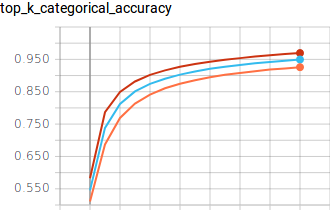
\includegraphics[width=0.5\linewidth]{part4/3CNN_train_top_k_accuracy}}
	\end{minipage}
	\hfill
	\begin{minipage}[ht]{1\linewidth}
		\center{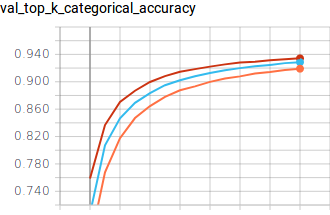
\includegraphics[width=0.5\linewidth]{part4/3CNN_val_top_k_accuracy}}
	\end{minipage}
	\caption{Models train and validation top k accuracy by epochs}
	\label{img:3CNN_top_k_accuracy}  
\end{figure}


\begin{figure}[ht] 
	\center
	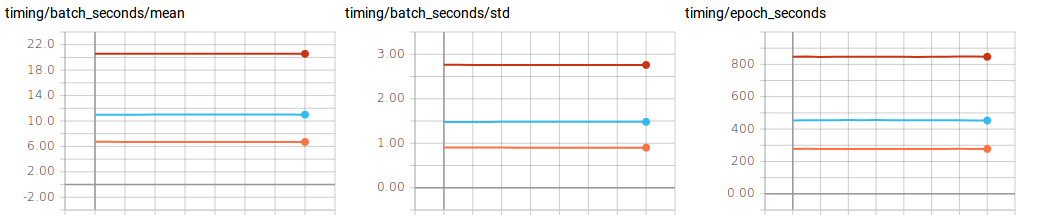
\includegraphics [scale=0.5] {part4/3CNN_timing}
	\caption{Models batch time by epochs} 
	\label{img:3CNN_timing}  
\end{figure}

\clearpage

Histograms of convolution layers Figure \ref{img:3CNN_conv_layers} look almost the same. They do not change significantly from the initial distribution. It can mean that layers do not learn much. 

\begin{figure}[ht]
	\begin{minipage}[ht]{1\linewidth}
		\center{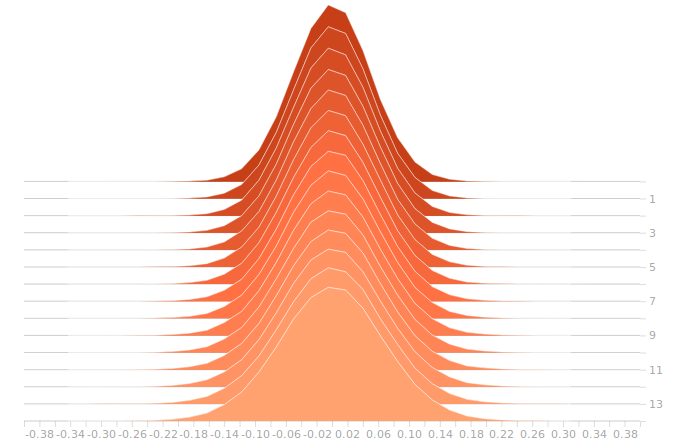
\includegraphics[width=0.5\linewidth]{part4/3CNN-conv-128.png} \\ а}
	\end{minipage}
	\hfill
	\begin{minipage}[ht]{1\linewidth}
		\center{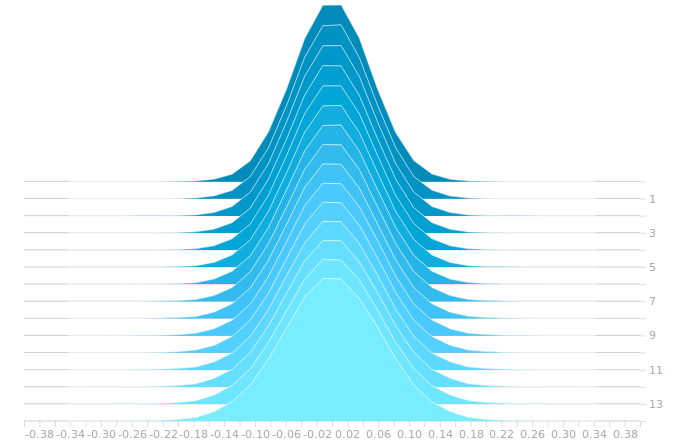
\includegraphics[width=0.5\linewidth]{part4/3CNN-conv-256.png} \\ b}
	\end{minipage}
	\begin{minipage}[ht]{1\linewidth}
		\center{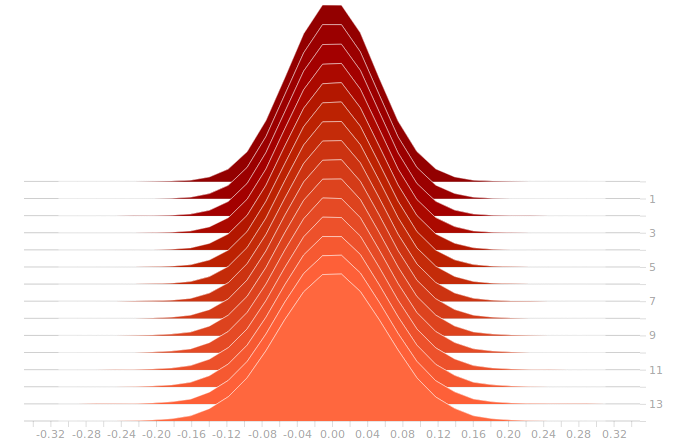
\includegraphics[width=0.5\linewidth]{part4/3CNN-conv-512.png} \\ c}
	\end{minipage}
	\caption{Convolutional model (a) 128;(b) 256; (c) 512 filters for each sizes [3, 4, 5]. Histogram of convolution layers}
	\label{img:3CNN_conv_layers}  
\end{figure}

\noindent
\\
\\
\\
\\
\\
Merged layers Figure \ref{img:3CNN_merged_layers} are also very similar, because of convolution layers.

\begin{figure}[ht]
	\begin{minipage}[ht]{1\linewidth}
		\center{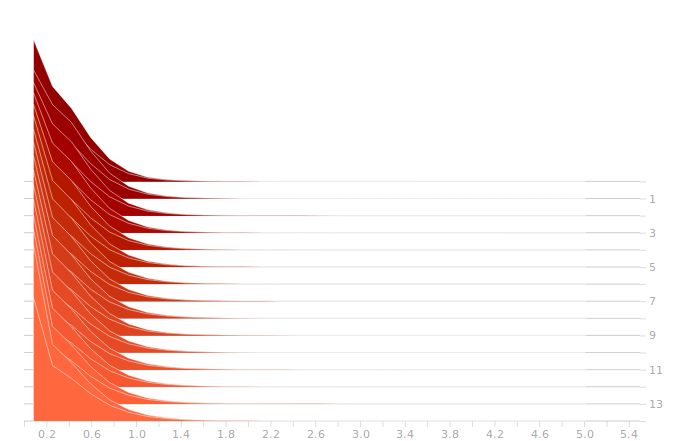
\includegraphics[width=0.45\linewidth]{part4/3CNN-merge3-128.png} \\ а}
	\end{minipage}
	\hfill
	\begin{minipage}[ht]{1\linewidth}
		\center{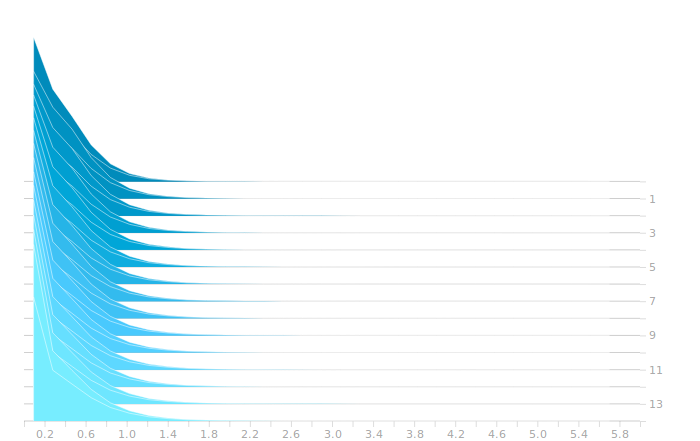
\includegraphics[width=0.45\linewidth]{part4/3CNN-merge3-256.png} \\ b}
	\end{minipage}
	\begin{minipage}[ht]{1\linewidth}
 		\center{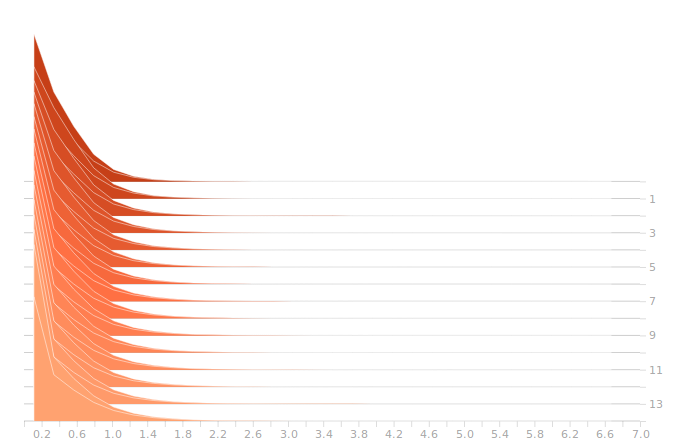
\includegraphics[width=0.45\linewidth]{part4/3CNN-merge3-512.png} \\ c}
	\end{minipage}
	\caption{Convolutional model (a) 128;(b) 256; (c) 512 filters for each sizes [3, 4, 5]. Histogram of merged layers}
	\label{img:3CNN_merged_layers}  
\end{figure}

\clearpage
We can easily notice the difference in the shape of the distribution Figure \ref{img:3CNN_dense_layers} on the initial epoch and the final. The model with 512 filters has a normal distribution with lower variance comparing to the one with 128 filters. It is noticeable, that the final distribution changed comparing to initial one, which means that layer learned some information. 

\begin{figure}[ht]
	\begin{minipage}[ht]{1\linewidth}
		\center{\includegraphics[width=0.5\linewidth]{part4/3CNN-dense-128.png} \\ а}
	\end{minipage}
	\hfill
	\begin{minipage}[ht]{1\linewidth}
		\center{\includegraphics[width=0.5\linewidth]{part4/3CNN-dense-256.png} \\ b}
	\end{minipage}
	\begin{minipage}[ht]{1\linewidth}
		\center{\includegraphics[width=0.5\linewidth]{part4/3CNN-dense-512.png} \\ c}
	\end{minipage}
	\caption{Convolutional model (a) 128;(b) 256; (c) 512 filters for each sizes [3, 4, 5]. Histogram of dense layers}
	\label{img:3CNN_dense_layers}  
\end{figure}

\clearpage
The CNN model requires fewer resources for training than bi-LSTM. Therefore, I was able to use 
5 times bigger batch size. We can see consumption of resources in Figure \ref{img:resources_CNN}

\begin{figure}[ht] 
	\center
	\includegraphics [scale=0.2] {part4/resources_CNN}
	\caption{CPU resources which were used while training CNN.} 
	\label{img:resources_CNN}  
\end{figure}




\clearpage
\section{Convolution neural network with different regularization} \label{sect4_4}

In this section, I tried to use different regularization to get rid of overfitting. I tested all these approaches on the CNN with 512 filters. I made the following changes in the initial architecture of the model:

%blue-modified_epoch15_outdim183_nbfilters512_drop10.5_drop20.2
%grey-withl2regul_0.001_0.01_adam_epoch15_outdim183_nbfilters512_drop10.25_drop20.25
%pink-withl2regul_0.001_0.01_epoch15_outdim183_nbfilters512_drop10.25_drop20.25
%cyan-withl2regul_epoch15_outdim183_nbfilters512_drop10.25_drop20.25


Modifications:
\begin{enumerate}
	\item In the previous section the convolution layer did not train enough,
	 was caused, in my opinion by a big dropout rate. Therefore, I decreased it in two times.
	\item I also added the l2-regularization equals to 0.01 both for convolution layers and dense layer. 
	Dropout equals to the rate 0.5 both for dense and convolution layers. 
	Moreover, I decided to configure my training algorithm, so I used Adam with learning rate 1e-4. 
	\item l2-regularization equals to 0.001 for convolution layers and 0.01 for dense layer. 
	Adam was with learning rate 1e-3. 
	Dropout rate equals to 0.25 both for dense and convolution layers. 
	\item l2-regularization equals to 0.001 for convolution layers and 0.01 for dense layers. 
	Dropout rate equals to 0.25 for convolution layers and 0.5 for dense layers.
\end{enumerate}

\begin{table}[h]
	\centering
	\caption{Analysis of categorical accuracy}
	\label{my-label}
	\begin{tabular}{| p{3cm} | p{3cm} | p{3cm} |}
		%	\begin{tabulary}{1.0\textwidth}{|L|L|L|L|L|L}
		\hline
		\textbf{Modification type}  & \textbf{Train} & \textbf{Test}                                                    
		\\ \hline
		1   &  0.8321 & 0.7993
		\\ \hline
		2   &  0.7101 & 0.7146 
		\\ \hline
		3   &  0.9026 & 0.7882
		\\ \hline		
		4   &  0.8514 & 0.7449
		\\ \hline
	\end{tabular}
\end{table}

\begin{table}[h]
	\centering
	\caption{Analysis of categorical cross entropy}
	\label{my-label}
	\begin{tabular}{| p{3cm} | p{3cm} | p{3cm} |}
		%	\begin{tabulary}{1.0\textwidth}{|L|L|L|L|L|L}
		\hline
		\textbf{Modification type}  & \textbf{Train} & \textbf{Test}                                                    
		\\ \hline
		1   &  0.7894 & 0.9405
		\\ \hline
		2   &   1.504 &  1.7040
		\\ \hline
		3   &  0.4928 & 1.4280
		\\ \hline		
		4   &  0.7151 & 1.6890
		\\ \hline
	\end{tabular}
\end{table}

\begin{table}[h]
	\centering
	\caption{Analysis of top k accuracy}
	\label{my-label}
	\begin{tabular}{| p{3cm} | p{3cm} | p{3cm} |}
		%	\begin{tabulary}{1.0\textwidth}{|L|L|L|L|L|L}
		\hline
		\textbf{Modification type}  & \textbf{Train} & \textbf{Test}                                                    
		\\ \hline
		1   &  0.9681 & 0.9348
		\\ \hline
		2  &   0.8333 & 0.8363
		\\ \hline
		3   &  0.9704 & 0.9179
		\\ \hline		
		4   &  0.9453 & 0.8921
		\\ \hline
	\end{tabular}
\end{table}

\noindent
\\
According to the results shown in Figures \ref{img:4CNN_categorical_accuracy}, \ref{img:4CNN_category_crossentropy}, \ref{img:4CNN_top_k_accuracy}, \ref{img:4CNN_timing}, it can be clearly seen that models with modifications number 3 and 4 were overfitted for sure.
Model number 1 has a lower overfit rate. The most stable model was number 2, which demonstrated the same results on test and train dataset. 

\begin{figure}[ht]
	\begin{minipage}[ht]{1\linewidth}
		\center{\includegraphics[width=0.5\linewidth]{part4/4CNN_train_category_accuracy}}
	\end{minipage}
	\hfill
	\begin{minipage}[ht]{1\linewidth}
		\center{\includegraphics[width=0.5\linewidth]{part4/4CNN_val_category_accuracy}}
	\end{minipage}
	\caption{Models train and validation categorical accuracy by epochs}
	\label{img:4CNN_categorical_accuracy}  
\end{figure}


\begin{figure}[ht]
	\begin{minipage}[ht]{1\linewidth}
		\center{\includegraphics[width=0.5\linewidth]{part4/4CNN_train_category_crossentropy}}
	\end{minipage}
	\hfill
	\begin{minipage}[ht]{1\linewidth}
		\center{\includegraphics[width=0.5\linewidth]{part4/4CNN_val_category_crossentropy}}
	\end{minipage}
	\caption{Models train and validation category crossentropy by epochs}
	\label{img:4CNN_category_crossentropy}  
\end{figure}

\begin{figure}[ht]
	\begin{minipage}[ht]{1\linewidth}
		\center{\includegraphics[width=0.5\linewidth]{part4/4CNN_train_top_k_accuracy}}
	\end{minipage}
	\hfill
	\begin{minipage}[ht]{1\linewidth}
		\center{\includegraphics[width=0.5\linewidth]{part4/4CNN_val_top_k_accuracy}}
	\end{minipage}
	\caption{Models train and validation top k accuracy by epochs}
	\label{img:4CNN_top_k_accuracy}  
\end{figure}

\begin{figure}[ht] 
	\center
	\includegraphics [scale=0.5] {part4/4CNN_timing}
	\caption{Models batch time by epochs} 
	\label{img:4CNN_timing}  
\end{figure}

 
\begin{figure}[ht]
	\begin{minipage}[ht]{1\linewidth}
		\center{\includegraphics[width=1\linewidth]{part4/4CNN-conv-1.png} \\ а, b}
	\end{minipage}
	\hfill
	\begin{minipage}[ht]{1\linewidth}
		\center{\includegraphics[width=1\linewidth]{part4/4CNN-conv-2.png} \\ c, d}
	\end{minipage}
	\caption{Convolutional models with modification (a) 1;(b) 2; (c) 3; (d) 4. Histogram of convolution layers}
	\label{img:Convolutional models with modification convolution layers}  
\end{figure}

\clearpage
If we compare results of weights histograms Figures \ref{img:Convolutional models with modification convolution layers}, \ref{img:Convolutional models with modification merged layers} with the ones in Section \ref{sect4_3} we can see a significant difference in distributions.
Which is mostly caused by different types of regularizations. We can also see that convolution layers from model 1 and 3 change through epochs, which
means that they learn.  

\begin{figure}[ht]
	\begin{minipage}[ht]{1\linewidth}
		\center{\includegraphics[width=1\linewidth]{part4/4CNN-merge3-1.png} \\ а, b}
	\end{minipage}
	\hfill
	\begin{minipage}[ht]{1\linewidth}
		\center{\includegraphics[width=1\linewidth]{part4/4CNN-merge3-2.png} \\ c, d}
	\end{minipage}
	\caption{Convolutional models with modification (a) 1;(b) 2; (c) 3; (d) 4. Histogram of merged layers}
	\label{img:Convolutional models with modification merged layers}  
\end{figure}

\clearpage
Similar situation can be seen with dense layers in Figure \ref{img:Convolutional models with modification Histogram of dense layers}. The weights are put into ranges between -0.1 and 0.1 where l2-regularizations were used.
The changes through epochs we can be seen only in first two models which are marked in blue and gray.   

\begin{figure}[ht]
	\begin{minipage}[ht]{1\linewidth}
		\center{\includegraphics[width=1\linewidth]{part4/4CNN-dense-1.png} \\ а, b}
	\end{minipage}
	\hfill
	\begin{minipage}[ht]{1\linewidth}
		\center{\includegraphics[width=1\linewidth]{part4/4CNN-dense-2.png} \\ c, d}
	\end{minipage}
	\caption{Convolutional models with modification (a) 1;(b) 2; (c) 3; (d) 4.  Histogram of dense layers}
	\label{img:Convolutional models with modification Histogram of dense layers}  
\end{figure}


As we can see regularizations play the key role to avoid the overfitting of the models. High dropout rate in combination with l2-regularization for dense and convolutions layers showed the best stability. Therefore, I chose model number 2 for the further training. 

\clearpage
\section{Final model} \label{sect4_5}

In this section I trained the best model from the Section \ref{sect4_5} on 25 epochs.
I have the following parameters:

\begin{itemize}
	\item 300 filters
	\item size of filter: 3, 4, 5
	\item l2-regularization equals to 0.01 both for convolution layers and dense layer. 
	\item dropout equals to the rate 0.5 both for dense and convolution layers. 
	\item learning algorithm Adam with learning rate 1e-4. 
\end{itemize}

One more modification which was made: from the previous Section \ref{sect4_5}
according to many metrics model with these configurations trained slower than others because 
it has the lowest learning rate 1e-4. To speed up the training process I increased the learning rate at the beginning to be equal 1e-3. Then as the CNN slowly converges to its optimal value
the learning was decreased to 1e-4 to slow down - otherwise it may overshoot the optimal value.
Such modifications gave me improvement in speed and the stability of the model at the same time.
The final results can be seen in Figures \ref{img:final_CNN_categorical_accuracy}, 
\ref{img:final_CNN_category_crossentropy}, \ref{img:final_CNN_top_k_accuracy}.


\begin{table}[h]
	\centering
	\caption{Final results}
	\label{my-label}
	\begin{tabular}{| p{7cm} | p{3cm} | p{3cm} |}
		%	\begin{tabulary}{1.0\textwidth}{|L|L|L|L|L|L}
		\hline
		\textbf{Metric}  & \textbf{Train} & \textbf{Test}                                                    
		\\ \hline
		categorical accuracy   &  0.8250 & 0.8307
		\\ \hline
		category crossentropy  &   0.5800 & 0.6612
		\\ \hline
		top k accuracy   &  0.9545 & 0.9473
		\\ \hline		
	\end{tabular}
\end{table}

	


\begin{figure}[ht]
	\begin{minipage}[ht]{1\linewidth}
		\center{\includegraphics[width=0.5\linewidth]{part4/final_CNN_train_category_accuracy}}
	\end{minipage}
	\hfill
	\begin{minipage}[ht]{1\linewidth}
		\center{\includegraphics[width=0.5\linewidth]{part4/final_CNN_val_category_accuracy}}
	\end{minipage}
	\caption{Models train and validation categorical accuracy by epochs}
	\label{img:final_CNN_categorical_accuracy}  
\end{figure}


\begin{figure}[ht]
	\begin{minipage}[ht]{1\linewidth}
		\center{\includegraphics[width=0.5\linewidth]{part4/final_CNN_train_category_crossentropy}}
	\end{minipage}
	\hfill
	\begin{minipage}[ht]{1\linewidth}
		\center{\includegraphics[width=0.5\linewidth]{part4/final_CNN_val_category_crossentropy}}
	\end{minipage}
	\caption{Models train and validation category crossentropy by epochs}
	\label{img:final_CNN_category_crossentropy}  
\end{figure}

\clearpage
\begin{figure}[ht]
	\begin{minipage}[ht]{1\linewidth}
		\center{\includegraphics[width=0.5\linewidth]{part4/final_CNN_train_top_k_accuracy}}
	\end{minipage}
	\hfill
	\begin{minipage}[ht]{1\linewidth}
		\center{\includegraphics[width=0.5\linewidth]{part4/final_CNN_val_top_k_accuracy}}
	\end{minipage}
	\caption{Models train and validation top k accuracy by epochs}
	\label{img:final_CNN_top_k_accuracy}  
\end{figure}


\begin{longtable}[c]{|l|c|c|l|l|}
	\caption[Classification report]{Classification report}
	\label{tab:amortecimentos_1}\\
	\hline  category & precision & recall &  f1-score & support\\ \hline
	\endhead
	\hline
	\endlastfoot
	
	1        & 0         & 0      & 0        & 7       \\
	3        & 0         & 0      & 0        & 4       \\
	4        & 0         & 0      & 0        & 2       \\
	11       & 0.78      & 0.58   & 0.66     & 623     \\
	14       & 0.93      & 0.99   & 0.96     & 8070    \\
	15       & 0.82      & 0.68   & 0.74     & 362     \\
	16       & 0.93      & 0.95   & 0.94     & 1656    \\
	20       & 0.82      & 0.91   & 0.86     & 1151    \\
	25       & 0.75      & 0.9    & 0.82     & 1910    \\
	29       & 0.97      & 0.99   & 0.98     & 12346   \\
\end{longtable}

Here is the concise version of final classification report for each class. Full version can be found in APPENDIX B. As we can see in the Table \ref{amortecimentos_1} model showed the best results on the categories with a big number of advertisements: 14, 29. It makes mistakes on categories with less samples: 11 and 15 respectively and can hardly ever make a right predictions on the categories where the number of observations are less than 10. 

\section{Summary of the section} \label{sect4_6}

In this section I have made a series of
experiments with recurrent and convolutional neural networks
built on top of word2vec. I did a little tuning
of hyperparameters to achieve the highest scores. 
According to the results of experiments which CNN models achieved, are the same and in some components even better than the ones of Bi-LSTM models.I can make a conclusion that Convolution Neural Networks perform remarkably well for NLP related problems and specially for text classification. 


           % Глава 4
\chapter*{CONCLUSIONS}						% Заголовок
\addcontentsline{toc}{chapter}{CONCLUSIONS}	% Добавляем его в оглавление

%% Согласно ГОСТ Р 7.0.11-2011:
%% 5.3.3 В заключении диссертации излагают итоги выполненного исследования, рекомендации, перспективы дальнейшей разработки темы.
%% 9.2.3 В заключении автореферата диссертации излагают итоги данного исследования, рекомендации и перспективы дальнейшей разработки темы.
%% Поэтому имеет смысл сделать эту часть общей и загрузить из одного файла в автореферат и в диссертацию:

%Основные результаты работы заключаются в следующем.
%%% Согласно ГОСТ Р 7.0.11-2011:
%% 5.3.3 В заключении диссертации излагают итоги выполненного исследования, рекомендации, перспективы дальнейшей разработки темы.
%% 9.2.3 В заключении автореферата диссертации излагают итоги данного исследования, рекомендации и перспективы дальнейшей разработки темы.
\begin{enumerate}
  \item На основе анализа \ldots
  \item Численные исследования показали, что \ldots
  \item Математическое моделирование показало \ldots
  \item Для выполнения поставленных задач был создан \ldots
\end{enumerate}

%И какая-нибудь заключающая фраза.
%This new approach works much better than simple Bag-of-Words words encoding and usage of basic classification algorithm.  

Representing words as vectors in the vector space in combination with Deep learning Neural Networks demonstrate high quality classification of textual data. The layers of NN get meaningful information of each class and can well distinguish one from another. In this thesis we proved that Convolution NNs can perform the same and in some components even better than Recurrent NNs and they are a right choice to work with textual data. Convolution NNs demonstrated high accuracy on unknown data with appropriate speed. However it is necessary to spend some time to pick the right regularization for layers to avoid overfitting problems.

Future work:
\begin{itemize}
	\item train networks with other training algorithms. For example, it is possible to try SGD or RMSprop with appropriate parameters. 
	\item make an assemble of neural networks to best use each one`s strong qualities.
	\item try to use different words sequences length for titles and descriptions
	\item as the results on categories were not really impressive it is possible to add them into one large called other'  
\end{itemize}      % Заключение
\clearpage                                  % В том числе гарантирует, что список литературы в оглавлении будет с правильным номером страницы
\phantomsection
\addcontentsline{toc}{chapter}{\bibname}	% Добавляем список литературы в оглавление
%\hypersetup{ urlcolor=black }               % Ссылки делаем чёрными
%\providecommand*{\BibDash}{}                % В стилях ugost2008 отключаем использование тире как разделителя 
\urlstyle{rm}                               % ссылки URL обычным шрифтом
\insertbiblioother                          % Подключаем Bib-базы
\urlstyle{tt}                               % возвращаем установки шрифта ссылок URL
%\hypersetup{ urlcolor={urlcolor} }          % Восстанавливаем цвет ссылок


\begin{thebibliography}
	{1} 
	\bibitem{jurafsky} Jurafsky D. Speech and Language Processing / D. Jurafsky, M. James   H. – New Jersey, 2008. – 1031 с. – (Pearson). – (ISBN: 0131873210). 
	 {2}
	 \bibitem{manning} Manning C. An Introduction to Information Retrieval / C. Manning, P. Raghavan, H. Schütze. – Cambridge, England: Online edition, 2009. – 544 p. – (Cambridge University Press).  (ISBN: 0521865719).
	 {3}
	 \bibitem{foundationsml}  Mohri M. Foundations of Machine Learning / M. Mohri, A. Rostamizadeh, A. Talwalkar. – Cambridge, Massachusetts, 2012. – 412 с. – (The MIT Press). – (ISBN: 9780262018258).
	 {4}
	 \bibitem{handsonml} Géron A. Hands-On Machine Learning with Scikit- Learn and TensorFlow / Aurélien Géron. – Gravenstein Highway North, Sebastopol, CA, 2017. – 751 с. – (O’Reilly Media). – (ISBN: 8009989938).
	 {5}
	 \bibitem{LR}Yang, Yiming, and Xin Liu. 1999. A re-examination of text categorization methods.
	 In Proc. SIGIR, pp. 42–49. ACM Press. 2
	 {}
	 \bibitem{NB1}McCallum, Andrew, and Kamal Nigam. 1998. A comparison of event models for
	 Naive Bayes text classification. In AAAI/ICML Workshop on Learning for Text Categorization,
	 pp. 41–48.
	 {}
	 \bibitem{NB2}Rennie, Jason D., Lawrence Shih, Jaime Teevan, and David R. Karger. 2003. Tackling
	 the poor assumptions of naive Bayes text classifiers. In Proc. ICML, pp. 616–623.
	 {}
	  \bibitem{svm}Tong, Simon, and Daphne Koller. 2001. Support vector machine active learning with
	 applications to text classification. JMLR 2:45–66
	 {}
	 \bibitem{info_retrievel}Zavrel, Jakub, Peter Berck, and Willem Lavrijssen. 2000. Information extraction by text classification: Corpus mining for features. In Workshop Information Extraction
	 Meets Corpus Linguistics. URL: www.cnts.ua.ac.be/Publications/2000/ZBL00. Held in
	 conjunction with LREC-2000.
	 {}
	 \bibitem{assignment1} Assignment 1[Course assignment]. (2016). Retrieved from http://cs224d.stanford.edu/assignment1/assignment1.pdf 
	 {}
	 \bibitem{cbow_skip} 
	    @ARTICLE{2013arXiv1301.3781M,
	 	author = {{Mikolov}, T. and {Chen}, K. and {Corrado}, G. and {Dean}, J.
	 	},
	 	title = "{Efficient Estimation of Word Representations in Vector Space}",
	 	journal = {ArXiv e-prints},
	 	archivePrefix = "arXiv",
	 	eprint = {1301.3781},
	 	primaryClass = "cs.CL",
	 	keywords = {Computer Science - Computation and Language},
	 	year = 2013,
	 	month = jan,
	 	adsurl = {http://adsabs.harvard.edu/abs/2013arXiv1301.3781M},
	 	adsnote = {Provided by the SAO/NASA Astrophysics Data System}
	 }	
	 \bibitem{CNN}
		@ARTICLE{2014arXiv1408.5882K,
	 	author = {{Kim}, Y.},
	 	title = "{Convolutional Neural Networks for Sentence Classification}",
	 	journal = {ArXiv e-prints},
	 	archivePrefix = "arXiv",
	 	eprint = {1408.5882},
	 	primaryClass = "cs.CL",
	 	keywords = {Computer Science - Computation and Language, Computer Science - Neural and Evolutionary Computing},
	 	year = 2014,
	 	month = aug,
	 	adsurl = {http://adsabs.harvard.edu/abs/2014arXiv1408.5882K},
	 	adsnote = {Provided by the SAO/NASA Astrophysics Data System}
	 	}	
	 \bibitem{CNN_habr}
		Kalinin S. (2017, December, 7). Convolution neural networks with python.[Blog post]. Retrieved from https://habrahabr.ru/company/ods/blog/344008/
	 
\end{thebibliography}
%https://academicguides.waldenu.edu/writingcenter/apa/references/examples      % Список литературы
\clearpage
\phantomsection
\renewcommand{\listfigurename}{LIST OF FIGURES}
\renewcommand{\listtablename}{LIST OF TABLES}
\addcontentsline{toc}{chapter}{\listfigurename}
\listoffigures									% Список изображений


%%% Список таблиц %%%
% (ГОСТ Р 7.0.11-2011, 5.3.10)
\clearpage
\phantomsection
\addcontentsline{toc}{chapter}{\listtablename}
\listoftables									% Список таблиц
\newpage           % Списки таблиц и изображений (иллюстративный материал)
\setcounter{chapstyle}{0}   
\renewcommand{\appendixname}{APPENDIX}
\appendix
%%% Правка оформления ссылок на приложения:
%http://tex.stackexchange.com/questions/56839/chaptername-is-used-even-for-appendix-chapters-in-toc
%http://tex.stackexchange.com/questions/59349/table-of-contents-with-chapter-and-appendix
%% требует двойной компиляции
%\addtocontents{toc}{\def\protect\cftchappresnum{\appendixname{} }%
%\setlength{\cftchapnumwidth}{\widthof{\cftchapfont\appendixname\cftchapaftersnum}}%
%}
%% Оформление заголовков приложений ближе к ГОСТ:
\sectionformat{\chapter}[display]{% Параметры заголовков разделов в тексте
    label=\appendixname\ \thechapter,% (ГОСТ Р 2.105, 4.3.6)
    labelsep=20pt,
}
%\renewcommand\thechapter{\Asbuk{chapter}} % Чтобы приложения русскими буквами нумеровались

%\chapter{Appendix} \label{AppendixA}
\chapter*{APPENDIX A ILLUSTRATIVE MATERIAL}							% Заголовок
\addcontentsline{toc}{chapter}{APPENDIX A ILLUSTRATIVE MATERIAL}
\begin{figure}[ht] 
	\center
	\includegraphics [scale=0.35] {presentation-01}
\end{figure}

\begin{figure}[ht] 
	\center
	\includegraphics [scale=0.35] {presentation-02.png}
\end{figure}

\begin{figure}[ht] 
	\center
	\includegraphics [scale=0.35] {presentation-03}
\end{figure}

\begin{figure}[ht] 
	\center
	\includegraphics [scale=0.35] {presentation-04}
\end{figure}

\begin{figure}[ht] 
	\center
	\includegraphics [scale=0.35] {presentation-05}
\end{figure}

\begin{figure}[ht] 
	\center
	\includegraphics [scale=0.35] {presentation-06}
\end{figure}

\begin{figure}[ht] 
	\center
	\includegraphics [scale=0.35] {presentation-07}
\end{figure}

\begin{figure}[ht] 
	\center
	\includegraphics [scale=0.35] {presentation-08}
\end{figure}

\begin{figure}[ht] 
	\center
	\includegraphics [scale=0.35] {presentation-09}
\end{figure}

\begin{figure}[ht] 
	\center
	\includegraphics [scale=0.35] {presentation-10}
\end{figure}

\begin{figure}[ht] 
	\center
	\includegraphics [scale=0.35] {presentation-11}
\end{figure}

\begin{figure}[ht] 
	\center
	\includegraphics [scale=0.35] {presentation-12}
\end{figure}

\begin{figure}[ht] 
	\center
	\includegraphics [scale=0.35] {presentation-13}
\end{figure}

\begin{figure}[ht] 
	\center
	\includegraphics [scale=0.35] {presentation-14}
\end{figure}

\begin{figure}[ht] 
	\center
	\includegraphics [scale=0.35] {presentation-15}
\end{figure}


\chapter*{APPENDIX B DATA SAMPLES}							% Заголовок
\addcontentsline{toc}{chapter}{APPENDIX B DATA SAMPLES}

\begin{figure}[ht] 
	\center
	\includegraphics [scale=0.2] {part4/cnn_architecture.png}
	\label{img:cnn_architecture}  
	\caption{Architectures of CNN model} 
\end{figure}



\begin{longtable}[c]{|l|c|c|l|l|}
	\caption[Classification report]{Classification report}
	\label{tab:amortecimentos}\\
	\hline  category & precision & recall &  f1-score & support\\ \hline
	\endhead
	\hline
	\endlastfoot
	
	1        & 0         & 0      & 0        & 7       \\
	3        & 0         & 0      & 0        & 4       \\
	4        & 0         & 0      & 0        & 2       \\
	5        & 0         & 0      & 0        & 1       \\
	6        & 0         & 0      & 0        & 6       \\
	7        & 0         & 0      & 0        & 1       \\
	8        & 0         & 0      & 0        & 2       \\
	9        & 0         & 0      & 0        & 2       \\
	11       & 0.78      & 0.58   & 0.66     & 623     \\
	12       & 0.63      & 0.42   & 0.5      & 281     \\
	14       & 0.93      & 0.99   & 0.96     & 8070    \\
	15       & 0.82      & 0.68   & 0.74     & 362     \\
	16       & 0.93      & 0.95   & 0.94     & 1656    \\
	17       & 0.81      & 0.88   & 0.84     & 550     \\
	18       & 0.73      & 0.73   & 0.73     & 314     \\
	19       & 0.82      & 0.9    & 0.86     & 263     \\
	20       & 0.82      & 0.91   & 0.86     & 1151    \\
	21       & 0.91      & 0.41   & 0.56     & 76      \\
	22       & 0.82      & 0.85   & 0.83     & 830     \\
	23       & 0.44      & 0.56   & 0.49     & 482     \\
	24       & 0         & 0      & 0        & 4       \\
	25       & 0.75      & 0.9    & 0.82     & 1910    \\
	26       & 0.76      & 0.84   & 0.8      & 310     \\
	27       & 0         & 0      & 0        & 5       \\
	29       & 0.97      & 0.99   & 0.98     & 12346   \\
	30       & 0.86      & 0.61   & 0.72     & 270     \\
	31       & 0.85      & 0.52   & 0.64     & 224     \\
	33       & 0.9       & 0.95   & 0.92     & 434     \\
	34       & 0.5       & 0.04   & 0.07     & 26      \\
	35       & 0.09      & 0.04   & 0.06     & 24      \\
	36       & 0.16      & 0.15   & 0.16     & 67      \\
	37       & 0.89      & 0.66   & 0.76     & 197     \\
	38       & 0.68      & 0.21   & 0.33     & 183     \\
	40       & 0.81      & 0.68   & 0.74     & 678     \\
	42       & 0.89      & 0.9    & 0.89     & 1298    \\
	43       & 0.71      & 0.81   & 0.76     & 782     \\
	44       & 0.84      & 0.95   & 0.89     & 1184    \\
	45       & 1         & 0.03   & 0.06     & 30      \\
	46       & 0.58      & 0.31   & 0.41     & 181     \\
	47       & 0         & 0      & 0        & 1       \\
	51       & 0.72      & 0.85   & 0.78     & 591     \\
	53       & 0.59      & 0.72   & 0.65     & 793     \\
	55       & 0.84      & 0.95   & 0.89     & 2471    \\
	56       & 0.63      & 0.59   & 0.61     & 537     \\
	57       & 0.86      & 0.72   & 0.79     & 163     \\
	59       & 0         & 0      & 0        & 2       \\
	60       & 0.67      & 0.59   & 0.63     & 231     \\
	61       & 0.7       & 0.5    & 0.58     & 113     \\
	62       & 0.63      & 0.58   & 0.6      & 67      \\
	64       & 1         & 0.79   & 0.88     & 14      \\
	65       & 0.76      & 0.44   & 0.55     & 117     \\
	66       & 1         & 0.21   & 0.35     & 28      \\
	67       & 0.52      & 0.37   & 0.43     & 122     \\
	70       & 0         & 0      & 0        & 4       \\
	71       & 0         & 0      & 0        & 22      \\
	72       & 0.75      & 0.19   & 0.31     & 31      \\
	73       & 0         & 0      & 0        & 1       \\
	74       & 0.59      & 0.73   & 0.65     & 146     \\
	75       & 0         & 0      & 0        & 3       \\
	76       & 0         & 0      & 0        & 18      \\
	78       & 0.57      & 0.75   & 0.65     & 83      \\
	79       & 0.38      & 0.4    & 0.39     & 92      \\
	80       & 0.2       & 0.1    & 0.13     & 21      \\
	81       & 0         & 0      & 0        & 6       \\
	82       & 0.22      & 0.64   & 0.32     & 85      \\
	83       & 0.49      & 0.53   & 0.51     & 78      \\
	84       & 0.24      & 0.25   & 0.24     & 16      \\
	85       & 0.68      & 0.61   & 0.64     & 87      \\
	86       & 0.57      & 0.53   & 0.55     & 32      \\
	87       & 0.2       & 0.14   & 0.17     & 7       \\
	88       & 0         & 0      & 0        & 1       \\
	89       & 0.75      & 0.33   & 0.46     & 27      \\
	90       & 0.53      & 0.47   & 0.5      & 49      \\
	91       & 0.63      & 0.39   & 0.48     & 83      \\
	92       & 0.58      & 0.28   & 0.38     & 25      \\
	93       & 0.42      & 0.29   & 0.34     & 52      \\
	94       & 0         & 0      & 0        & 12      \\
	95       & 0.5       & 0.18   & 0.27     & 11      \\
	96       & 0.65      & 0.48   & 0.55     & 23      \\
	97       & 0         & 0      & 0        & 4       \\
	98       & 0.2       & 0.12   & 0.15     & 17      \\
	99       & 0         & 0      & 0        & 5       \\
	100      & 0.43      & 0.11   & 0.18     & 107     \\
	101      & 0.36      & 0.21   & 0.27     & 47      \\
	102      & 0.22      & 0.11   & 0.15     & 18      \\
	103      & 0         & 0      & 0        & 7       \\
	104      & 0.56      & 0.6    & 0.58     & 47      \\
	105      & 0.46      & 0.6    & 0.52     & 10      \\
	106      & 0         & 0      & 0        & 3       \\
	107      & 0.8       & 0.6    & 0.69     & 68      \\
	108      & 0.71      & 0.14   & 0.23     & 37      \\
	109      & 0.09      & 0.04   & 0.06     & 73      \\
	110      & 0         & 0      & 0        & 1       \\
	111      & 0.79      & 0.75   & 0.77     & 88      \\
	112      & 0.68      & 0.38   & 0.49     & 50      \\
	113      & 0.76      & 0.61   & 0.68     & 83      \\
	114      & 0.78      & 0.64   & 0.7      & 11      \\
	115      & 0.39      & 0.64   & 0.49     & 194     \\
	116      & 0.58      & 0.52   & 0.55     & 87      \\
	117      & 0.41      & 0.33   & 0.37     & 21      \\
	118      & 0.81      & 0.73   & 0.77     & 237     \\
	119      & 0.63      & 0.63   & 0.63     & 70      \\
	120      & 0.67      & 0.56   & 0.61     & 18      \\
	121      & 0         & 0      & 0        & 4       \\
	122      & 0.6       & 0.54   & 0.57     & 28      \\
	123      & 0.55      & 0.89   & 0.68     & 63      \\
	124      & 0.74      & 0.84   & 0.78     & 87      \\
	125      & 0.65      & 0.57   & 0.61     & 56      \\
	126      & 0.63      & 0.7    & 0.67     & 47      \\
	127      & 0.67      & 0.57   & 0.62     & 7       \\
	128      & 0.62      & 0.36   & 0.46     & 22      \\
	129      & 0.8       & 0.5    & 0.62     & 8       \\
	130      & 0         & 0      & 0        & 4       \\
	131      & 0.64      & 0.46   & 0.53     & 167     \\
	132      & 0.72      & 0.5    & 0.59     & 62      \\
	133      & 1         & 0.2    & 0.33     & 5       \\
	134      & 0.66      & 0.72   & 0.69     & 87      \\
	135      & 0.64      & 0.78   & 0.7      & 18      \\
	136      & 1         & 0.25   & 0.4      & 8       \\
	137      & 0.8       & 0.85   & 0.82     & 142     \\
	138      & 0.76      & 0.62   & 0.69     & 56      \\
	139      & 0.31      & 0.31   & 0.31     & 83      \\
	140      & 0         & 0      & 0        & 1       \\
	141      & 0.33      & 0.09   & 0.14     & 81      \\
	142      & 0.37      & 0.34   & 0.35     & 263     \\
	143      & 0         & 0      & 0        & 5       \\
	144      & 0.62      & 0.15   & 0.24     & 66      \\
	145      & 0.78      & 0.83   & 0.8      & 142     \\
	146      & 0.47      & 0.2    & 0.28     & 35      \\
	147      & 0.53      & 0.7    & 0.6      & 221     \\
	148      & 0.56      & 0.25   & 0.34     & 109     \\
	149      & 0.29      & 0.18   & 0.22     & 11      \\
	150      & 0         & 0      & 0        & 12      \\
	151      & 0         & 0      & 0        & 34      \\
	152      & 0         & 0      & 0        & 89      \\
	153      & 0         & 0      & 0        & 4       \\
	154      & 0.81      & 0.29   & 0.43     & 58      \\
	155      & 0         & 0      & 0        & 35      \\
	156      & 0.57      & 0.18   & 0.27     & 68      \\
	157      & 0.21      & 0.1    & 0.14     & 30      \\
	158      & 0.76      & 0.88   & 0.82     & 375     \\
	159      & 0.57      & 0.09   & 0.16     & 43      \\
	160      & 0.43      & 0.59   & 0.49     & 188     \\
	162      & 0.62      & 0.56   & 0.58     & 263     \\
	165      & 0.71      & 0.67   & 0.69     & 445     \\
	166      & 0.53      & 0.37   & 0.43     & 49      \\
	167      & 0         & 0      & 0        & 13      \\
	168      & 0.92      & 0.93   & 0.93     & 423     \\
	169      & 0.83      & 0.91   & 0.87     & 570     \\
	172      & 0.71      & 0.67   & 0.69     & 625     \\
	249      & 0.57      & 0.46   & 0.51     & 177     \\
	250      & 0.28      & 0.08   & 0.13     & 109     \\
	251      & 0.78      & 0.74   & 0.76     & 316     \\
	252      & 0.56      & 0.62   & 0.59     & 332     \\
	253      & 0.65      & 0.67   & 0.66     & 313     \\
	254      & 0.71      & 0.18   & 0.28     & 299     \\
	255      & 0.87      & 0.79   & 0.83     & 232     \\
	256      & 0.76      & 0.57   & 0.65     & 312     \\
	257      & 0.88      & 0.91   & 0.89     & 847     \\
	258      & 0.57      & 0.72   & 0.64     & 495     \\
	259      & 0.89      & 0.75   & 0.81     & 63      \\
	265      & 0.69      & 0.92   & 0.79     & 101     \\
	266      & 0.62      & 0.78   & 0.69     & 233     \\
	267      & 0.62      & 0.42   & 0.5      & 31      \\
	268      & 0.64      & 0.77   & 0.7      & 258     \\
	269      & 0         & 0      & 0        & 17      \\
	270      & 0.74      & 0.55   & 0.63     & 158     \\
	272      & 0.8       & 0.79   & 0.79     & 228     \\
	273      & 0.62      & 0.21   & 0.31     & 78      \\
	274      & 0.63      & 0.33   & 0.44     & 108     \\
	275      & 0.93      & 0.42   & 0.58     & 31      \\
	278      & 0.78      & 0.5    & 0.61     & 129     \\
	279      & 0.79      & 0.86   & 0.82     & 842     \\
	280      & 0.57      & 0.47   & 0.51     & 344     \\
	281      & 0.62      & 0.6    & 0.61     & 419     \\
	283      & 0         & 0      & 0        & 23      \\
	284      & 0.83      & 0.4    & 0.54     & 248     \\
	285      & 0.67      & 0.03   & 0.06     & 66      \\
	287      & 0.56      & 0.58   & 0.57     & 429     \\
	288      & 0         & 0      & 0        & 66      \\
	289      & 0         & 0      & 0        & 80      \\
	avg      & 0.81      & 0.82   & 0.81     & 55000  
\end{longtable}
        % Приложения

\end{document}
